% Автоматически перенесено из ГЛАВА_1_ВЕРСИЯ_3.docx

\chapter{Вычислительный метод выявления текстуальных связей в правовых памятниках Каталонии XII--XIII~вв.}

Письменные памятники каталонского обычного права XII--XIII~вв. формировались не изолированно: зафиксированные в них нормы и правовые формулы могли быть связаны с предшествующей латинской традицией, другими каталонскими сводами и практикой составления актов. Однако текстуальное сходство между источниками может иметь различную природу: оно способно указывать на почти дословное воспроизведение нормы, использование устойчивой формулы, переработку общей конструкции или принадлежность текстов к единой правовой традиции. Поэтому выявление совпадений должно сопровождаться анализом их распределения между памятниками и последующей проверкой по исходным фрагментам.

Цель главы состоит в выявлении и исторической интерпретации текстуальных связей между источниками латинской правовой традиции, каталонскими сводами обычного права и актовым материалом. Для достижения этой цели решаются три взаимосвязанные задачи: разрабатывается и обосновывается воспроизводимый вычислительный метод отбора потенциальных соответствий; определяется структура связей «Барселонских обычаев» с более ранними латинскими текстами, другими каталонскими сборниками и грамотами; наиболее значимые совпадения сопоставляются с исходными текстами, чтобы установить степень и возможный характер их родства.

Для решения поставленных задач используется алгоритм, объединяющий структурное членение источников, предварительную обработку текста, отбор потенциальных соответствий, расчёт нескольких показателей близости, парето-фильтрацию, ранжирование и графовую репрезентацию результатов. Вычислительный анализ рассматривается при этом как инструмент предварительного поиска и систематизации материала: установленная алгоритмом близость сама по себе не доказывает прямого заимствования, а указывает на фрагменты, требующие источниковедческой и историко-филологической проверки.

Техническая реализация метода зафиксирована в открытом репозитории GitHub, где хранятся основные компоненты исследования --- исходные тексты источников, конфигурационный файл с описанием режимов экспериментов, программный код основного пайплайна\footnote{В данном исследовании термин «пайплайн» используется для обозначения целостной вычислительной процедуры, организованной как последовательность формализованных этапов, каждый из которых выполняет определённую аналитическую функцию и передаёт результат на последующую стадию обработки.}, корпус-специфические модули структурного членения, вспомогательные скрипты тестирования, а также автоматически формируемые материалы по итогам экспериментов\footnote{AnnaIasinskaia. Usatges\_de\_Barcelona [Электронный ресурс]. URL: \url{https://github.com/AnnaIasinskaia/Usatges\_de\_Barcelona} (дата обращения: 09.04.2026).}. Подобная организация репозитория позволяет документировать не только результаты исследования, но и всю последовательность операций, лежащих в его основе. Центральное место в ней занимает конфигурационный файл config.py, в котором в явном виде заданы состав корпусов, параметры предварительной обработки, логика предварительного отбора, глубина парето-фильтрации, правила агрегации и настройки визуализации. Тем самым постановка каждого эксперимента фиксируется в виде отдельной и воспроизводимой конфигурации, что позволяет сопоставлять результаты экспериментов на строго формализованной основе.

Для работы алгоритма используются библиотеки numpy, scipy, networkx, matplotlib, python-Levenshtein и python-docx, обеспечивающие соответственно численные вычисления, расчёт статистических и метрических показателей, построение и экспорт структур графов, визуализацию результатов, операции формального сопоставления строк и подготовку текстовых выходных файлов. В то же время следует специально оговорить, что отдельные языковые инструменты, потенциально применимые к латинскому материалу, в частности simplemma и pycollatinus\footnote{Данное программное обеспечение распространяется свободно (бесплатно) и доступно по следующему адресу: \url{https://outils.biblissima.fr/en/collatinus}.URL: \url{https://outils.biblissima.fr/en/collatinus}. Дата обращения: 05.04.2020.}, в ходе работы продемонстрировали нестабильность и потому не могут рассматриваться как надёжная основа для автоматической обработки в рамках настоящего проекта. По этой причине в реализованной версии алгоритма акцент был перенесён с полной словарной лемматизации на более устойчивые процедуры нормализации и редукции словоформ, адаптированные к особенностям конкретных текстов. Подобное решение представляется методически обоснованным, поскольку позволяет обеспечить стабильность обработки на неоднородном историческом материале и одновременно избежать зависимости от внешних лексикографических модулей, чувствительных к орфографической вариативности, дефектам оцифровки и смешению языковых слоёв (github.com).

Результаты вычислительных экспериментов сохраняются в нескольких взаимодополняющих формах.

Во-первых, формируются табличные выходы, в которых фиксируются отдельные пары сегментов и значения рассчитанных для них метрик.

Во-вторых, создаются визуальные представления в виде графов, экспортируемые в файлы форматов CSV, GEXF и PNG, что делает возможным как последующий машинный анализ, так и визуальное рассмотрение структуры связей между корпусами и сегментами.

В-третьих, автоматически формируются markdown-отчёты, предназначенные для человекочитаемого представления результатов эксперимента: они содержат перечни наиболее сильных соответствий, идентификаторы сегментов, значения метрик, а в ряде случаев --- и текстовые примеры, позволяющие соотнести вычислительный результат с конкретным содержанием источника\footnote{См. приложение 3 к настоящей диссертации.}.

Тем самым результаты исследования оказались представлены в нескольких аналитических формах, каждая из которых выполняет собственную функцию --- проверку, интерпретацию, визуализацию и последующее сопоставление результатов между экспериментами.

\section{Метод построения генеалогии правовых текстов Каталонии XII--XIII~вв.}

Внутренняя логика предложенного метода определяется последовательным преодолением тех методологических трудностей, которые неизбежно возникают при сопоставлении исторических текстов различной природы. Сравнение текстов «Свода гражданского права» Юстиниана, «Этимологий» Исидора Севильского, «Барселонских обычаев», других каталонских сборников обычного права и грамот IX--XI и XII~вв. требует установить, что именно выступает сопоставимой единицей анализа --- статья, глава, обычай, грамота или иной структурный фрагмент. Не менее важно согласовать масштаб исследования с реальным объёмом и внутренней организацией этих единиц, поскольку локальное заимствование может проявляться как в пределах целой статьи, так и на её сравнительно небольшом отрезке. Дальнейшее сопоставление предполагает также предварительное приведение материала к устойчивому аналитическому виду: текст источников должен быть очищен от издательских помет и редакторских примечаний, нормализован и преобразован таким образом, чтобы сохранить содержательные различия между фрагментами. Принципиально важно, что в настоящем исследовании нормализация не подменяет источниковый текст и не претендует на текстологическую редакцию памятника. Она формирует вспомогательное, аналитическое представление сегмента, предназначенное для первичного вычислительного сопоставления. Все содержательные выводы о заимствовании, совпадении формулы или характере текстовой связи далее проверяются по исходным фрагментам источника, доступным по опубликованным изданиям\footnote{Проблема заключается в том, что рукописи и их транскрипции интересующих нас текстов в большинстве случаев оставались для нас недоступными.}.

Поскольку полное попарное сравнение всех сегментов корпуса было бы чрезмерно вычислительно затратным и методологически не обоснованным, необходим этап предварительного отбора наиболее правдоподобных соответствий. Наконец, итог исследования не может сводиться к простому набору числовых значений: задача состоит в том, чтобы перевести вычислительно найденные совпадения в интерпретируемую картину текстуальных связей, пригодную для историко-филологического анализа.

Таким образом, настоящее исследование организовано как последовательность семи взаимосвязанных этапов анализа:

определение структурной единицы сравнения;

уточнение масштаба анализа;

приведение текста к устойчивому аналитическому представлению;

предварительное сокращение пространства сопоставления;

расчёт различных метрик текстуальной близости;

отбор и упорядочивание результатов в многомерном пространстве признаков;

визуализация результатов.

Каждый последующий этап опирается на решения, принятые на предыдущем, поэтому итоговая картина текстуальных связей предстаёт как итог последовательного и методически контролируемого анализа.

\subsection{Выделение базовых структурных единиц сравнения}

Первый этап имеет принципиальное значение, поскольку именно здесь определяется, какая единица текста будет выступать объектом дальнейшего сопоставления. На первый взгляд эта задача может показаться преимущественно технической и сводимой к механическому разбиению источника на более или менее регулярные фрагменты, пригодные для последующей обработки. Однако применительно к текстам исторических источников, в особенности правового характера, подобное решение почти неизбежно приведёт к методологическому искажению. Внутренняя организация таких памятников лишь в редких случаях совпадает с обозначенными издателями границами страницы, абзаца или даже печатного заголовка. Поэтому сопоставление целого документа со случайно выделенным фрагментом главы, одной нормы с частью соседней нормы или основного текста с блоком, включающим редакторский аппарат, изначально смещает предмет исследования и подменяет содержательное сравнение формальным.

На этом этапе нам пришлось столкнуться с рядом трудностей. Прежде всего, внешняя разметка источника далеко не всегда совпадает с его внутренней структурой: нумерация издания, абзацные членения и печатные заголовки могут служить полезными ориентирами, но сами по себе ещё не гарантируют, что выделяемый фрагмент действительно соответствует исторически осмысленной единице текста. Не менее существенна проблема неоднородности текста. Во многих источниках основной текст сосуществует с критическим аппаратом, примечаниями, поздними вставками, глоссами, переводами и иными редакционными наслоениями. Эти элементы способны существенно исказить результаты сравнительного анализа и даже сделать его вовсе не информативным. Наконец, особое значение имеет устойчивая идентификация сегментов. Выделенные единицы должны быть не только формально разграничены, но и снабжены такими обозначениями, которые были бы одновременно уникальными, стабильными и содержательно связанными со структурой источника. Это необходимо как для последующих вычислительных операций, так и для интерпретации результатов: когда обозначение отсылает к конкретной статье, обычаю или иному структурному элементу, исследователь сохраняет связь между аналитической процедурой и текстом как историческим источником.

На материале «Барселонских обычаев» значение первого этапа проявляется особенно отчётливо. В данном случае недостаточно механически ориентироваться на нумерацию статей, поскольку в цифровом представлении корпуса основной латинский текст соседствует с каталанским, издание Ж.~Бастардеса-и-Пареры снабжено массивным критическим аппаратом --- сиглами рукописей, примечаниями, редакторскими вставками и пояснениями. Поэтому задача сводится к выделению собственно правового текста из окружающих его вторичных слоёв. Соответственно, используемый для этого памятника модуль структурного членения должен извлекать основной латинский фрагмент, исключая элементы, не принадлежащие ему в строгом текстологическом смысле. В историко-текстологической перспективе такое решение означает, что объектом сравнения становится не весь текст «Барселонских обычаев» (с комментариями, уточнениями и редакторскими пометами), а последовательность отдельных статей, которые в дальнейшем будут сопоставляться с аналогичными структурными элементами других источников.

Именно на первом этапе каждому выделенному сегменту (в случае «Барселонских обычаев» --- статье) присваивается не только собственный идентификатор, но и поле parent\_id. В техническом отношении оно фиксирует исходную структурную единицу, к которой относится данный фрагмент текста. Пока сегмент ещё не подвергался дальнейшему дроблению, его собственный идентификатор и parent\_id совпадают, поскольку в этот момент он сам выступает как исходная единица анализа. Это означает, что уже на первом этапе алгоритм не только выделяет отдельную статью, главу или грамоту, но и сохраняет указание на этот фрагмент как на базовую структурную основу всех последующих операций. Благодаря этому при дальнейшем разбиении крупных сегментов на более мелкие части каждый такой дочерний фрагмент может быть однозначно соотнесён с тем обычаем, статьёй или документом, из которого он был получен. Тем самым parent\_id обеспечивает связь между локальным вычислительным уровнем анализа и уровнем исторически осмысленной текстовой единицы.

\subsection{Дробление крупных сегментов на перекрывающиеся окна}

После того как на первом этапе определена базовая единица сравнения, возникает следующий методологический вопрос: в какой мере эта единица действительно пригодна для непосредственного сопоставления с сегментами, выделенными в других источниках? Материал исторических корпусов показывает, что в большинстве случаев такая единица не может автоматически считаться оптимальной. Часть сегментов, полученных на предыдущем этапе, оказывается достаточно компактной и внутренне однородной, вследствие чего они могут непосредственно использоваться в дальнейшем анализе. Иные сегменты, напротив, отличаются значительным объёмом и включают несколько смысловых блоков, что затрудняет их сопоставление. В подобных случаях локальное текстуальное совпадение может быть скрыто общим объёмом фрагмента и потому остаться нераспознанным. Именно этим обусловлена необходимость второго этапа, задача которого состоит в контролируемом расчленении крупных сегментов на перекрывающиеся текстовые окна.

Следует особо подчеркнуть, что речь не идёт о механическом дроблении всего корпуса на единообразные по размеру части. Смысл данного этапа заключается не в формальном измельчении текста, а в уточнении аналитического масштаба, на котором сопоставление становится наиболее продуктивным. С одной стороны, единица анализа должна быть достаточно объёмной, чтобы вмещать значимый контекст, устойчивую формулу и содержательно важный фрагмент текста. С другой стороны, она не должна быть чрезмерно крупной, поскольку в этом случае локальное заимствование или текстуальные совпадения могут утратить различимость внутри более общего массива словесного материала. По этой причине дробление применяется лишь в тех случаях, когда оно действительно необходимо, а его параметры --- длина окна, степень перекрытия и минимальный порог сегмента --- определяются не произвольно, а с учётом распределения длины сегментов в конкретном корпусе.

В техническом отношении данная процедура реализуется как построение скользящего окна по последовательности слов. Исходный сегмент предварительно переводится в словесную последовательность, после чего на её основе формируются окна заданной длины с частичным взаимным перекрытием. Наличие перекрытия имеет принципиальное значение, поскольку оно предотвращает потерю содержательно значимого фрагмента на границе двух соседних окон. Если же сегмент невелик по объёму или уже соответствует заданному размеру окна, он сохраняется в исходном виде и дополнительному дроблению не подвергается. Тем самым второй этап не отменяет результатов первого, а выполняет функцию их уточнения: одни сегменты сохраняются без изменений, другие переводятся в более чувствительную форму локального сопоставления. Такое решение особенно существенно при работе с неоднородными корпусами, где длина структурных единиц может существенно варьировать.

Принципиальным результатом второго этапа становится формирование двухуровневой иерархии сегментов. Исходная статья, глава, обычай или грамота сохраняется как базовая структурная единица, тогда как возникающие в результате дробления окна выступают как её производные элементы. Именно в этом контексте поле parent\_id обретает своё полное функциональное значение. Если сегмент подвергается дроблению, каждое образованное окно получает собственный идентификатор, однако parent\_id продолжает указывать на исходный более крупный сегмент. Иначе говоря, каждый новый фрагмент сохраняет однозначную связь с той структурной единицей, из которой он был выделен. Для исследователя это означает, что совпадение может быть обнаружено на уровне отдельного окна, но затем соотнесено с исходной статьёй, обычаем или иным более крупным элементом текста. Без такой связи анализ неизбежно замыкался бы на уровне мелких и слабо интерпретируемых фрагментов, что существенно осложняло бы последующее историко-филологическое осмысление результатов.

На материале «Барселонских обычаев» значение второго этапа проявляется особенно наглядно, поскольку данный корпус показывает, что дробление не должно превращаться в самоцель. Во многих случаях отдельные статьи уже представляет собой естественную, завершённую и достаточно компактную единицу анализа. При таких условиях автоматическое разделение всех обычаев на окна не только не повысило бы точность сопоставления, но и могло бы снизить его интерпретируемость. Именно на втором этапе происходит согласование вычислительного масштаба анализа с реальной структурой источника, не разрушая при этом его внутренней организации.

\subsection{Предварительная обработка и редукция текста}

Если первый этап задаёт корректную структурную единицу сравнения, второй --- адекватный масштаб сопоставления, то третий этап обеспечивает перевод исторического текста в устойчивую аналитическую форму, пригодную для последующей вычислительной обработки. Именно на нём устанавливаются правила различения между содержательно значимыми особенностями текста и теми вариациями, которые обусловлены орфографической неустойчивостью, морфологической изменчивостью, редакторским вмешательством либо техническими дефектами оцифровки. В рамках предлагаемого подхода она представляет собой многоступенчатую процедуру, ориентированную на работу с неоднородным корпусом и направленную на формирование сопоставимого аналитического представления текста.

На начальном подэтапе выполняется техническая очистка текста от элементов, не относящихся непосредственно к тексту источника. Удаляются мягкие переносы и распознаваемые по формальным шаблонам обозначения пагинации, фолиации, сносок и редакционно-издательского аппарата (например, [12], fol. 25r, p. 10, cap. IV). Части слов, разделённые мягкими переносами, соединяются (например, \emph{constitu}\emph{-\textbackslash{}n }\emph{erunt} $\rightarrow$ \emph{constituerunt}). Одновременно строка приводится к стандартной форме Unicode для латинского или старокаталанского языка соответственно. Такая обработка уменьшает влияние особенностей набора и редакционного оформления на последующее сопоставление текстов.

После очистки выполняется токенизация, то есть разбиение текста на дискретные аналитические единицы --- токены\footnote{Manning Ch.D., Raghavan P., Schütze H. Introduction to Information Retrieval. Cambridge: Cambridge Unicersity Press, 2008. P.~23--24.}. Под токеном в данном случае понимается минимальная единица текстовой последовательности, с которой непосредственно работают последующие процедуры обработки. В зависимости от принятых правил такой единицей может выступать слово, числовое обозначение или иная формально выделяемая единица записи. Однако применительно к историческому материалу одного лишь механического членения текста недостаточно. Принципиально важным становится следующий подэтап --- определение режима сегмента, то есть предварительная классификация фрагмента по его языковым и формальным признакам.

На этом этапе наши действия исходят из предпосылки о языковой неоднородности текстов исторических источников. На предварительном этапе каждый сегмент соотносится с одним из трёх режимов: латинским, каталонским или связанным с дефектами оптического распознавания текста. Такая классификация необходима потому, что в пределах одного и того же текста в рамках мультилингвизма могут сосуществовать фрагменты, различающиеся по языку, графическому облику, степени сохранности и характеру редакционных наслоений. Лишь после установления того, к какому из этих трёх типов относится конкретный сегмент, становится возможной содержательно обоснованная нормализация текста.

После технической очистки различные формы графической записи приводятся к единообразному виду. Строка переводится в нижний регистр, снимаются диакритические знаки, лигатуры раскрываются (\emph{Æ} $\rightarrow$ \emph{ae}, \emph{œ} $\rightarrow$ \emph{oe}), а разные начертания апострофа и тире заменяются стандартными символами (\emph{’}, \emph{`}, \emph{´} $\rightarrow$ \emph{'}; \emph{---}, \emph{--}, \emph{−} $\rightarrow$ \emph{-}). Графические варианты \emph{j/i} и \emph{v/u} последовательно приводятся к \emph{i} и \emph{u}: \emph{judicium} $\rightarrow$ \emph{iudicium}, \emph{venerit} $\rightarrow$ \emph{uenerit}, \emph{privato} $\rightarrow$ \emph{priuato}. Апостроф внутри словоформы сохраняется, тогда как случайные апострофы в начале или в конце токена удаляются. Нормализация сокращает вариативность, обусловленную особенностями набора и издательской передачи текста, не предполагая исправления самого чтения источника.

Для латинских, романских и смешанных сегментов применяется общий набор графических преобразований. Более осторожная редукция романских и смешанных форм осуществляется на последующей стадии стемминга, где используется ограниченный перечень окончаний и более строгие требования к длине сохраняемой основы. Сегменты с выраженными признаками ошибок оптического распознавания обрабатываются отдельно: программа не восстанавливает предполагаемое правильное чтение, а снижает влияние вероятных технических искажений посредством более строгой фильтрации токенов. Исправление таких чтений возможно только при ручной сверке с изданием или изображением источника.

За нормализацией следует редукция словоформ посредством стемминга\footnote{Ibid. P.~32--34.}. Алгоритм отсекает отдельные флективные и словообразовательные окончания при соблюдении следующих требований:

\begin{itemize}
\item минимальная длина основы не менее трёх символов;
\item сохранение хотя бы одной гласной в основе;
\item недопустимость удаления, приводящего к совпадению с общеязыковыми служебными морфемами;
\item приоритет сохранения корневых согласных кластеров.
\end{itemize}
Это сокращает вариативность, затрудняющую выявление лексических соответствий: например, \emph{possit} и \emph{posse} приводятся к основе \emph{poss}, \emph{uoluerit} и \emph{uoluerunt} --- к \emph{uoluer}.

Редукция сопровождается частичной утратой морфологической информации и не всегда последовательно объединяет формы одной лексемы: \emph{tollere} преобразуется в \emph{tolle}, \emph{tollit} --- в \emph{toll}; \emph{fuerit} --- в \emph{fuer}, \emph{fuerint} --- в \emph{fueri}. Это повышает чувствительность поиска и одновременно вносит погрешность в оценку сходства. Поэтому редуцированное представление используется для выявления и ранжирования возможных соответствий, а их интерпретация проводится по исходным словоформам и контексту с учётом утраченных грамматических различий\footnote{Подробнее о различном значении наклонений глаголов в контексте анализа правовых памятников Средневековья см. \emph{Варьяш О.И.}~Язык средневекового права // \emph{Варьяш О.И.}~Пиренейские тетради: право, общество, власть и человек в средние века. Москва: Наука, 2006. С.~90.}.

В отличие от лемматизации, предполагающей обращение к словарным ресурсам и соотнесение каждой словоформы с её словарной формой, выбранный нами подход не опирается на внешние лексикографические модули\footnote{Ibid. P.~34.}. Такое решение было принято, поскольку готовые модули лемматизации\footnote{Например, Collatinus. [Электронный ресурс]. URL: \url{https://outils.biblissima.fr/en/collatinus} (дата обращения: 05.04.2026).} на средневековых текстах работают недостаточно устойчиво. Результат редукции с их применением напрямую зависит от полноты исходного словаря и от степени соответствия конкретной словоформы нормативной модели языка. Напротив, используемый в данном исследовании стемминг был предварительно откалиброван применительно к нашему кругу источников и показал более устойчивое поведение. Его задача состоит в последовательном снижении флективной и орфографической вариативности до такого уровня, при котором содержательная близость между сегментами становится вычислительно различимой.

Завершается данный этап фильтрацией токенов, исключением из дальнейшего анализа единиц с низкой информативностью и форм, с высокой вероятностью представляющих собой технический или текстовый шум. Удаляются токены короче трёх символов, а также частотные служебные слова --- союзы \emph{et}\emph{, }\emph{aut}\emph{, }\emph{sed}\emph{, }\emph{nec}\emph{, }\emph{neque}\emph{ }и др.; предлоги \emph{in, }\emph{ad}\emph{, de, }\emph{ex}\emph{, }\emph{ab}\emph{, }\emph{per}\emph{, }\emph{sine}\emph{ }и др.; относительные и вопросительные местоимения \emph{qui}\emph{, }\emph{quod}\emph{, }\emph{quis}\emph{, }\emph{quid}; указательные формы \emph{hic}\emph{, }\emph{ille}\emph{, }\emph{ipse}; личные и возвратные формы \emph{ego}\emph{, }\emph{tu}\emph{, }\emph{se}\emph{, }\emph{sibi}. Исключаются также по каким-либо причинам не удалённые из текста обозначения издательского аппарата, например \emph{cod}\emph{., }\emph{ms}\emph{., }\emph{fol}\emph{., }\emph{pag}\emph{., }\emph{cap}\emph{.}, и токены с признаками искажения --- сочетания букв и цифр, повторения одного и того же символа, последовательности согласных при полном отсутствии гласных.

Важно подчеркнуть, что полученная форма представляет собой не исправленный текст источника, а его вспомогательную аналитическую запись. Например, начальный и конечный фрагменты статьи Us.~111~(123) проходят следующую последовательность преобразований:

\begin{equation*}
\begin{aligned}
&\text{CONSTITVERVNT \ldots{} uoluerit \ldots{} possit}\;\longrightarrow\\
&\text{constituerunt \ldots{} uoluerit \ldots{} possit}\;\longrightarrow\\
&\text{constituerunt \ldots{} uoluer \ldots{} poss}.
\end{aligned}
\end{equation*}

На первом переходе унифицируется графическая запись, на втором сокращается часть окончаний. При содержательной проверке исследователь возвращается к исходному чтению; редуцированная форма нужна лишь для того, чтобы орфографическая и морфологическая вариативность меньше мешала поиску возможных соответствий.

\begin{center}
\small
\setlength{\tabcolsep}{2pt}
\begin{longtable}{|p{\dimexpr0.94\textwidth/5\relax}|p{\dimexpr0.94\textwidth/5\relax}|p{\dimexpr0.94\textwidth/5\relax}|p{\dimexpr0.94\textwidth/5\relax}|p{\dimexpr0.94\textwidth/5\relax}|}
\caption{Пример последовательной предварительной обработки текста на латинском языке (статья 111 (123) «Барселонских обычаев» --- фрагмент)}\label{tab:ch1-preprocessing}\\
\hline
 & \textbf{Исходный текст} & \textbf{Нормализ}\textbf{ация} & \textbf{Стемми}\textbf{нг} & \textbf{Итоговый набор токенов} \\ \hline
\textbf{Текст} & CONSTITVERVNT IGITVR ut si quis cum aliquo ierit uel fuerit, siue in uia, aut in domo, siue in agro, seu in alio quolibet loco, si aliquis inde eum requisierit uel aliquid de suo ei tollere uoluerit, adiu-\par 5 uet eum prout melius possit & constituerunt igitur ut si quis cum aliquo ierit uel fuerit si ue in uia aut in domo si ue in agro seu in alio quolibet loco si aliquis inde eum requisierit uel aliquid de suo ei tollere uoluerit adiu 5 uet eum prout melius possit & constituerunt igi ut si quis cum aliquo ier uel fuer si ue in uia aut in domo si ue in agro seu in alio quolibet loco si aliqu inde eum requisierit uel aliquid de suo ei tolle uoluer adiu 5 uet eum prout melius poss & constituerunt igi quis aliquo ier fuer uia domo agro seu alio quolibet loco aliqu eum requisierit aliquid tolle uoluer adiu uet prout melius poss \\ \hline
\textbf{Изменения} & --- & --- & igitur $\rightarrow$ igi; ierit $\rightarrow$ ier; fuerit $\rightarrow$ fuer; aliquis $\rightarrow$ aliqu; tollere $\rightarrow$ tolle; uoluerit $\rightarrow$ uoluer; possit $\rightarrow$ poss & Удалены служебные слова ut, si, cum, uel, ue, in, aut, inde, de, suo, ei, eum, а также номер строки --- 5 \\ \hline
\end{longtable}
\end{center}

На этом этапе создаётся редуцированная последовательность токенов для каждого выделенного сегмента из текстов. Именно это представление образует уровень, на котором далее вычисляются показатели текстового сходства. Предварительная обработка текста, с одной стороны, устраняет помехи, возникающие вследствие графической, языковой и технической вариативности материала источников, с другой --- сохраняет структурные и лексические характеристики текста, необходимые для выявления содержательных совпадений. В этом смысле она выступает переходным этапом от текста исторического источника как сложного и многослойного объекта к его вычислительно сопоставимому представлению.

\subsection{Предварительный отбор возможных соответствий}

После завершения первых трёх этапов корпус оказывается представлен в качестве множества сегментов, уже приведённых к сопоставимому виду. Возникает следующая задача --- организация пространства сравнений. Теоретически возможно сопоставление каждого сегмента в пределах одного корпуса с каждым сегментом всех остальных по всему набору последующих показателей. Однако при реальном объёме материала подобное полное попарное сравнение оказывается чрезмерно затратным по времени и вычислительным возможностям ПК, а потому практически неприменимым. Именно поэтому на четвёртом этапе проводится предварительный отбор возможных соответствий, назначение которого состоит в сокращении пространства анализа до ограниченного и вычислительно управляемого множества пар.

Мы использовали представление TF-IDF (англ. \emph{term}\emph{ }\emph{frequency}\emph{ --- }\emph{inverse}\emph{ }\emph{document}\emph{ }\emph{frequency}), способ «взвешивания» словесных единиц, при котором вес того или иного токена определяется, с одной стороны, частотой его употребления в данном сегменте, а с другой --- степенью его распространённости во всём корпусе. Так наибольшую значимость получают единицы, сравнительно характерные для данного текста и не слишком частотные в корпусе в целом\footnote{\emph{Chow~T.W.}S., Zhang H., \emph{Rahman M.K.} A new document representation using term frequency and vectorized graph connectionists with application to document retrieval // Expert Systems with Applications. 2009. Т.~36, №~10. P.~12025.}. В рамках предлагаемого подхода TF-IDF не рассматривается ни как окончательная мера заимствования, ни как самостоятельное основание для вывода о текстуальном родстве. Эта статистическая мера служит инструментом первичного отбора, позволяющим быстро выделить те пары сегментов, в которых уже обнаруживается некоторая степень общей лексической близости. Этот подход особенно эффективен для устранения заведомо бессодержательных сопоставлений и для сохранения тех случаев, где наблюдается пересечение по информативным словам или устойчивым кратким сочетаниям. Вместе с тем, TF-IDF-представление по своему характеру фиксирует главным образом векторное и лексическое сходство\footnote{Aizawa A. An information theoretic perspective of TF-IDF measures // Information Processing \& Management. 2003. Т.~39, №~1. P.~46.}. Тем самым мы разграничиваем две задачи --- предварительное выделение возможных соответствий и собственно оценку степени текстовой близости.

Логику вычисления можно разложить на три простых действия. Пусть $t$ обозначает токен или короткое сочетание токенов, а $d$ --- один сегмент. Через $f(t,d)$ обозначим, сколько раз $t$ встречается в $d$. Чтобы частотность не зависела напрямую от длины сегмента, это число делится на наибольшую частоту какого-либо токена $u$ в том же сегменте:

\begin{equation}
\operatorname{tf}(t,d)=\frac{f(t,d)}{\max\limits_{u\in d} f(u,d)}.
\end{equation}

Здесь буква $u$ не обозначает особый вид слова: она последовательно принимает значения всех токенов сегмента $d$, а выражение в знаменателе выбирает наибольшую из их частот. Далее учитывается редкость токена в корпусе. Пусть $N$ --- общее число сегментов, а $\operatorname{df}(t)$ --- число сегментов, в которых встретился $t$. Тогда

\begin{equation}
\operatorname{idf}(t)=\ln\frac{N}{\operatorname{df}(t)},
\end{equation}

где $\ln$ обозначает натуральный логарифм. Итоговый вес получается умножением двух величин:

\begin{equation}
w(t,d)=\operatorname{tf}(t,d)\,\operatorname{idf}(t).
\end{equation}

Например, если слово встретилось в сегменте два раза, а самое частое слово --- четыре раза, то $\operatorname{tf}=2/4=0{,}5$. Если это слово присутствует в пяти сегментах из ста, то $\operatorname{idf}=\ln(100/5)\approx3$. Его итоговый вес будет приблизительно равен $0{,}5\cdot3=1{,}5$. Тем самым повторяющееся внутри данного фрагмента, но редкое в корпусе слово получает заметный вес.

В техническом отношении по всем сегментам сопоставляемых текстов строится общее TF-IDF-представление, учитывающее отдельные токены, а также последовательности из двух и трёх токенов. Признаки, встретившиеся менее чем в двух сегментах или более чем в половине сегментов, при построении этого представления исключаются. Векторы весов приводятся к единому масштабу посредством L2-нормализации: каждый вес делится на квадратный корень из суммы квадратов всех весов данного сегмента. После этого длина каждого ненулевого вектора условно равна 1, и различие в объёме сегментов меньше влияет на сравнение. На основе этих векторов для пар сегментов вычисляется косинусная близость, после чего сохраняется ограниченное число наиболее перспективных пар-кандидатов. В эксперименте сопоставления латинских источников с «Барселонскими обычаями» это ограничение задано в конфигурационном файле как вычислительный бюджет предварительного отбора. Всего после объединения результатов может быть передано на последующие стадии не более 5000 пар, при этом для каждой пары источников задаётся минимальный бюджет в 300 кандидатов, а число кандидатов, приходящихся на один сегмент левой стороны, дополнительно ограничивается значением 12.

Под вычислительным бюджетом здесь понимается техническое ограничение на число пар, которые допускаются к более ресурсоёмкому анализу на следующих этапах. Полный попарный расчёт всех последующих мер близости для всех сегментов был бы избыточным по времени (занимал бы несколько сотен часов) и вычислительно нерациональным для возможностей ПК. Поэтому четвёртый этап решает задачу предварительного поиска и формирует достаточно широкий набор пар-кандидатов, заслуживающих дальнейшей проверки.

При пороговом подходе исследователь должен был бы заранее объявить универсальное значение косинусной близости, выше которого пары считаются значимыми, например 0,3 или 0,4. Для разнородных по своей природе правовых текстов (записи обычного права, грамоты и др.) такой порог трудно мотивировать: длина сегментов, степень сохранности текста, язык, графическая вариативность и плотность устойчивых правовых формул могут существенно различаться. Окончательная оценка пары переносится на следующие этапы, где учитываются несколько независимых мер сходства, парето-фильтрация, ранжирование и последующая содержательная проверка исходных фрагментов.

Этот этап исследования обеспечивает его вычислительную реализуемость, не подменяя при этом предварительный отбор окончательным выводом о степени текстового родства. Именно на нём закладывается статистическая основа для ряда последующих показателей, поскольку здесь рассчитываются веса информативности токенов. С одной стороны, этот этап существенно сокращает пространство сопоставлений, с другой --- подготавливает аналитическую базу для последующего многомерного рассмотрения результатов. При отсутствии этой стадии вычисление более сложных показателей для полного множества пар сегментов было бы либо чрезмерно ресурсоёмким, либо методически неоправданным.

\subsection{Расчёт мер текстовой близости}

На пятом этапе каждая пара сегментов, прошедшая предварительный отбор, получает не единичную, а многокомпонентную характеристику текстовой близости. Такое решение определяется самой природой исследуемого явления. Возможное текстуальное соответствие в исторических корпусах может проявляться на нескольких уровнях --- в виде общего лексического сходства, совпадения редкой и содержательно значимой лексики, частичного совпадения вариативных словоформ или наличия локально воспроизводимого пассажа. Вследствие этого использование одной универсальной меры не обеспечило бы методологической строгости, а, напротив, привело бы к чрезмерному упрощению материала и к утрате части значимых соответствий. Вычислительный результат на этом этапе обозначает именно возможное соответствие; вывод о текстуальной связи и тем более о заимствовании требует последующей источниковедческой проверки.

Первая из используемых мер --- косинусная близость TF-IDF-представлений\footnote{Salton G., Buckley C. Term-weighting approaches in automatic text retrieval // Information Processing \& Management. 1988. Т.~24, №~5. P.~513--523.}. Если на предыдущем этапе она применялась как инструмент предварительного отбора, то здесь она выступает уже как одна из полноправных характеристик пары сегментов. Её аналитическая ценность состоит в том, что она позволяет зафиксировать общий лексико-фразовый фон сходства между ними. В тех случаях, когда два фрагмента разделяют значимую часть словаря и кратких словесных сочетаний, данный показатель принимает высокие значения. Вместе с тем эта мера слабо чувствительна к линейной организации текста и практически не различает ситуации, в которых совпадающие элементы образуют единый локальный пассаж, и ситуации, в которых они лишь распределены по всему сегменту. Следовательно, она обладает значительной эвристической ценностью, однако её использование не является достаточным для исчерпывающего решения поставленной задачи.

Вторая мера ориентирована на пересечение по редкой и содержательно значимой лексике и условно обозначается как Tesserae. Она восходит к подходам, разработанным в исследованиях интертекстуальности\footnote{Coffee N. et al. The Tesserae Project: intertextual analysis of Latin poetry // Literary and Linguistic Computing. 2013. Т.~28, №~2. P.~221--228; \emph{Gawley J.O.}, \emph{Diddams A.C.}~Comparing the intertextuality of multiple authors using Tesserae: A new technique for normalization // Digital Scholarship Humanities. 2017. Т.~32, Is. Suppl.\_2. P. ii53--ii59.}. В данном случае значимым оказывается не количество общих единиц, а совпадение тех токенов, которые встречаются сравнительно редко и потому обладают большей диагностической силой. Для историко-филологического анализа такая мера особенно важна, поскольку позволяет выделять не всякое сходство словаря, а именно те совпадения, которые обладают повышенной содержательной нагрузкой. Наличие нескольких общих редких и характерных единиц нередко оказывается более весомым аргументом в пользу возможной текстуальной связи, чем высокая степень общего лексического сходства как такового.

Третья мера --- мягкая косинусная близость\footnote{Sidorov~G. et al. Soft Similarity and Soft Cosine Measure Similarity of Features in Vector Space Model // Computación y Sistemas. 2014. Vol.~18, №. 3. P.~494.} --- вводится для учёта не только полных совпадений, но и частичного формального сходства между словоформами. Для исторических текстов это имеет принципиальное значение, поскольку даже после нормализации в текстах исторических источников сохраняются орфографические и морфологические варианты. В подобных случаях две единицы не могут быть признаны тождественными, но и не должны рассматриваться как полностью различные. Мягкая косинусная близость позволяет учитывать частичный вклад таких форм в общий профиль сходства пары и тем самым повышает чувствительность метода к вариативности письма, редакционной переработке и неполному совпадению словесной формы.

Наконец, четвёртая мера основана на локальном выравнивании последовательностей Смита --- Уотермана\footnote{Этот подход был впервые применён в работах по молекулярной биологии для выравнивания последовательностей белков и в дальнейшем адаптирован к историко-лингвистическим задачам: \emph{Smith T.F., Waterman M.S}. Identification of common molecular subsequences // Journal of Molecular Biology. 1981. Vol.~147, no. 1. P.~195--197. DOI: 10.1016/0022-2836(81)90087-5; \emph{Smith T.F., Waterman M.S., Fitch W.M. }Comparative biosequence metrics // Journal of Molecular Evolution. 1981. Vol.~18, no. 1. P.~38--46. DOI: 10.1007/BF01733210;\emph{ }\emph{Katrenko}\emph{ S., Adriaans P., van~Someren M. }Using local alignments for relation recognition // Journal of Artificial Intelligence Research. 2010. Vol.~38, Is.~1. P.~1--48.}. В отличие от трёх предшествующих, ориентированных преимущественно на множественные или векторные представления текста, она направлена на выявление наилучшего совпадающего локального фрагмента. Именно это делает её особенно значимой для анализа возможных заимствований, поскольку исторически существенная связь между двумя правовыми сегментами нередко выражается не в сходстве текста в целом, а в воспроизведении конкретного локального оборота, устойчивой формулы или структурно близкой конструкции. Процедура локального выравнивания позволяет выявить именно такие случаи. Итоговый показатель нормируется, чтобы результаты можно было сопоставлять между парами сегментов разной длины.

Для большей определённости используемые меры близости далее зафиксированы в аналитическом виде. Формулы нужны не для подмены исторической интерпретации, а для точного описания того, что именно вычисляет программа. Пусть $x$ и $y$ обозначают два сравниваемых сегмента после предварительной обработки. Под сегментом здесь понимается сравнительно небольшой фрагмент текста, например \emph{«Priuilegia autem sunt leges priuatorum…»}\footnote{Usatges de Barcelona. Us. D2 (140): «\textbf{Priuilegia autem sunt leges priuatorum}, quasi priuate leges; nam priuilegium inde dictum, quod in priuato feratur». P.~173.}, тогда как токеном выступает отдельная аналитическая единица вроде \emph{testes}, \emph{imperari}, \emph{priuilegia} или \emph{priuato}.

\textbf{Первая мера} --- \textbf{косинусная близость TF-IDF-представлений}. Пусть $m$ --- общее число признаков в TF-IDF-представлении, то есть отдельных токенов и учитываемых коротких сочетаний. Буква $i$ обозначает порядковый номер такого признака, а $w_{i,x}$ и $w_{i,y}$ --- его TF-IDF-веса в сегментах $x$ и $y$. Знак $\sum$ означает, что стоящие после него величины складываются для всех признаков с номерами от 1 до $m$. Тогда косинусная близость вычисляется по формуле

\begin{equation}
\operatorname{Cos}(x,y)=
\frac{\displaystyle\sum_{i=1}^{m}w_{i,x}w_{i,y}}
{\displaystyle
\sqrt{\sum_{i=1}^{m}w_{i,x}^{2}}
\sqrt{\sum_{i=1}^{m}w_{i,y}^{2}}}.
\end{equation}

Числитель увеличивается, когда одни и те же признаки имеют заметный вес в обоих сегментах. Две суммы под квадратными корнями учитывают общий объём весов каждого сегмента и позволяют сопоставлять фрагменты разной длины. Величина, близкая к 1, соответствует очень сходному распределению признаков; величина, близкая к 0, --- слабому сходству.

\textbf{Вторая мера} ориентирована на \textbf{пересечение по редкой} и содержательно значимой \textbf{лексике}. Обозначим через $C_{xy}$ набор токенов, общих для сегментов $x$ и $y$, а через $c_{xy}$ --- число таких общих токенов. Наконец, $n_x$ и $n_y$ обозначают число уникальных токенов соответственно в $x$ и $y$. Используемая в работе мера Tesserae вычисляется следующим образом:

\begin{equation}
\operatorname{Tess}(x,y)=
\begin{cases}
\dfrac{\displaystyle\sum_{t\in C_{xy}}\operatorname{idf}(t)}
{\sqrt{n_xn_y}}, & \text{если }c_{xy}\geq2;\\[8pt]
0, & \text{если }c_{xy}<2.
\end{cases}
\end{equation}

В числителе складываются уже введённые выше веса редкости $\operatorname{idf}(t)$ всех общих токенов. Деление на $\sqrt{n_xn_y}$ ослабляет влияние размера сегментов. Дополнительное условие требует не менее двух общих уникальных токенов: единичное совпадение, даже по редкому слову, не получает положительной оценки. Это авторская мера, построенная по принципу Tesserae, а не воспроизведение всей системы Tesserae; поэтому её значения не следует понимать как вероятность и они могут превышать 1. Если после предварительной обработки у двух сегментов обнаруживаются общие токены \emph{imperari}, \emph{idonei}, \emph{uidentur}, \emph{fiant}, \emph{testes}, \emph{quibus}, \emph{potest}, именно их редкость и число определяют высокое значение данной меры.

\textbf{Третья мера} --- это \textbf{мягкая косинусная близость}. Она учитывает не только полные совпадения токенов, но и их частичное формальное сходство. В отличие от первой меры, здесь используются не TF-IDF-веса, а обычные частоты токенов. Пусть $m$ --- число различных токенов в общем словаре двух сегментов; $i$ и $j$ --- порядковые номера двух токенов этого словаря; $c_{x,i}$ --- число появлений токена $i$ в сегменте $x$, а $c_{y,j}$ --- число появлений токена $j$ в сегменте $y$. Через $s(i,j)$ обозначим формальную близость двух токенов. Тогда

\begin{equation}
\operatorname{SoftCos}(x,y)=
\frac{
\displaystyle\sum_{i=1}^{m}\sum_{j=1}^{m}c_{x,i}c_{y,j}s(i,j)}
{\sqrt{
\left(\displaystyle\sum_{i=1}^{m}\sum_{j=1}^{m}c_{x,i}c_{x,j}s(i,j)\right)
\left(\displaystyle\sum_{i=1}^{m}\sum_{j=1}^{m}c_{y,i}c_{y,j}s(i,j)\right)}}.
\end{equation}

Двойная сумма означает, что каждый токен первого сегмента сопоставляется с каждым токеном второго. Чтобы определить $s(i,j)$, используется расстояние Левенштейна $d_L(i,j)$ --- минимальное число вставок, удалений и замен букв, необходимое для превращения одного токена в другой. Через $\ell(i)$ обозначим число букв в токене $i$, а запись $\max(\ell(i),\ell(j))$ означает выбор длины более длинного из двух токенов. В используемой реализации

\begin{equation}
s(i,j)=
\begin{cases}
1, & \text{если }i=j;\\[3pt]
1-\dfrac{d_L(i,j)}{\max\bigl(\ell(i),\ell(j)\bigr)},
& \text{если }i\neq j\text{ и }d_L(i,j)\leq2;\\[8pt]
0, & \text{если }d_L(i,j)>2.
\end{cases}
\end{equation}

Полностью совпадающие токены получают близость 1. Формы, различающиеся не более чем двумя редакционными операциями, получают промежуточное значение; при большем различии их сходство считается нулевым. Например, формы \emph{nichil} и \emph{nihil} различаются одной операцией: $d_L=1$, длина более длинной формы равна 6, поэтому их формальная близость составляет $1-1/6\approx0{,}83$. Сопоставление \emph{calumpnia} и \emph{calumnia} оценивается по тому же правилу. Это не доказывает исторической связи само по себе, но позволяет не утратить её из-за небольшой графической вариации.

Наконец, \textbf{четвёртая мера} основана на \textbf{локальном выравнивании последовательностей}. В данном случае сравниваются не только сегменты целиком, но и их локальные фрагменты. Если, например, один сегмент содержит цепочку токенов \emph{idonei}, \emph{uidentur}, \emph{testes}, \emph{quibus}, \emph{imperari}, \emph{potest}, \emph{testes}, \emph{fiant}, а другой --- близкую последовательность \emph{idonei}, \emph{testes}, \emph{uidentur}, \emph{quibus}, \emph{imperari}, \emph{potest}, \emph{testes}, \emph{fiant}, алгоритм ищет наиболее сильный совпадающий участок, даже если вокруг него тексты различаются.

Пусть первый сегмент представлен последовательностью $x=(a_1,\ldots,a_{L_x})$, а второй --- последовательностью $y=(b_1,\ldots,b_{L_y})$. Здесь $a_i$ и $b_j$ --- токены на позициях $i$ и $j$, а $L_x$ и $L_y$ --- длины сегментов в токенах. Для вычисления строится таблица $H$: её ячейка $H_{i,j}$ хранит лучшую оценку локального совпадения, заканчивающегося на токенах $a_i$ и $b_j$. Нулевая строка и нулевой столбец таблицы заполняются нулями, а остальные ячейки вычисляются по правилу

\begin{equation}
H_{i,j}=\max
\begin{cases}
0,\\
H_{i-1,j-1}+\sigma(a_i,b_j),\\
H_{i-1,j}-1,\\
H_{i,j-1}-1.
\end{cases}
\end{equation}

Первый вариант начинает новый локальный участок; второй продолжает сопоставление двух токенов; третий и четвёртый учитывают пропуск токена в одной из последовательностей со штрафом $-1$. Функция $\sigma(a_i,b_j)$ задаёт оценку сопоставления двух токенов. При полном совпадении она равна 2; при небольшом различии, когда расстояние Левенштейна не превышает 2, используется плавно уменьшающаяся положительная оценка; во всех остальных случаях ставится штраф $-1$:

\begin{equation}
\sigma(a_i,b_j)=
\begin{cases}
2, & \text{если }a_i=b_j;\\[3pt]
2\left(1-\dfrac{d_L(a_i,b_j)}
{\max\bigl(\ell(a_i),\ell(b_j)\bigr)}\right),
& \text{если }a_i\neq b_j\text{ и }d_L(a_i,b_j)\leq2;\\[8pt]
-1, & \text{если }d_L(a_i,b_j)>2.
\end{cases}
\end{equation}

Ненормированная оценка $\operatorname{SW}(x,y)$ равна наибольшему значению во всей таблице $H$, то есть оценке лучшего локального участка. Для сопоставления сегментов разной длины используется нормированная форма:

\begin{equation}
\operatorname{SW}_{\mathrm{norm}}(x,y)=
\frac{\operatorname{SW}(x,y)}{\max\bigl(1,\min(L_x,L_y)\bigr)}.
\end{equation}

Запись $\min(L_x,L_y)$ означает длину меньшего сегмента; внешняя операция $\max(1,\ldots)$ предотвращает деление на ноль для пустого фрагмента. Поскольку каждое точное совпадение добавляет 2 балла, $\operatorname{SW}_{\mathrm{norm}}$ может превышать 1. Следовательно, это нормированная сравнительная оценка, а не вероятность и не доля совпавшего текста.

Совместное использование этих четырёх мер означает, что каждая пара сегментов получает собственный многомерный профиль сходства. Один случай может характеризоваться общей лексической близостью, другой --- пересечением по редкой лексике, третий --- совпадением вариативных форм, четвёртый --- наличием структурно сходного пассажа. В центре исследовательского внимания находится выявление тех соответствий, которые оказываются сильными в многомерном пространстве признаков. Именно такая постановка делает метод чувствительным к разнообразию форм текстового родства и освобождает его от чрезмерной зависимости от выбора единственной меры.

\subsection{Многослойная парето-фильтрация и ранжирование}

После завершения пятого этапа каждая пара сегментов характеризуется несколькими мерами близости, вследствие чего пространство анализа существенно усложняется. С одной стороны, такая многомерность позволяет точнее описывать различные формы текстового родства, с другой --- затрудняет последующий отбор, поскольку простое упорядочение всех пар по одному показателю неизбежно привело бы к утрате значительной части содержательно важных различий. Вместе с тем сохранение всего массива многомерных результатов без дополнительного сокращения также не представляется возможным, поскольку в этом случае итоговое множество соответствий оказывается чрезмерно объёмным и слабо поддаётся интерпретации. Разрешение данного противоречия обеспечивается посредством многослойной парето-фильтрации с последующим ранжированием.

Для того чтобы избежать преждевременного сведения всех показателей к одной шкале, каждая пара сегментов на данном этапе рассматривается как носитель четырёх значений, соответствующих ранее введённым мерам близости. Иначе говоря, профиль пары $P$ можно записать в виде

\begin{equation}
M(P)=\bigl(\operatorname{Cos}(P),\operatorname{Tess}(P),
\operatorname{SoftCos}(P),\operatorname{SW}_{\mathrm{norm}}(P)\bigr).
\end{equation}

Буква $P$ здесь обозначает не отдельный текст, а одну конкретную пару сравниваемых сегментов; $M(P)$ --- четыре полученные для неё оценки.

Парето-фильтрация основывается на отношении доминирования в многомерном пространстве признаков\footnote{Kang S., Li K., Wang R. A survey on pareto front learning for multi-objective optimization // Journal of Membrane Computing. 2025. Т.~7, №~2. P.~128--134.}. Сравним две пары, обозначенные $P$ и $Q$. Пара $P$ доминирует над парой $Q$, если она не слабее по каждой из четырёх мер:

\begin{equation}
\begin{aligned}
\operatorname{Cos}(P)&\geq\operatorname{Cos}(Q),\\
\operatorname{Tess}(P)&\geq\operatorname{Tess}(Q),\\
\operatorname{SoftCos}(P)&\geq\operatorname{SoftCos}(Q),\\
\operatorname{SW}_{\mathrm{norm}}(P)&\geq\operatorname{SW}_{\mathrm{norm}}(Q).
\end{aligned}
\end{equation}

При этом хотя бы одно из четырёх неравенств должно быть строгим: по меньшей мере одна оценка пары $P$ должна быть выше соответствующей оценки пары $Q$. Если все четыре значения равны, пары равносильны, но ни одна из них не доминирует над другой. Это уточнение принципиально: одного условия «не хуже по всем показателям» недостаточно.

Если для некоторой пары существует такая доминирующая альтернатива, данная пара не попадает в первый слой. Пары, для которых доминирующей альтернативы нет, образуют первый парето-слой. После его удаления та же процедура применяется к оставшемуся множеству: так выделяются второй, третий и последующие слои\footnote{\emph{Pérez-Piqueras V., López P}\emph{.}\emph{B., }\emph{Gámez}\emph{ J.A. }Estimation of distribution algorithms with solution subset selection for the next release problem // Log J IGPL. 2025. Т.~33, №~5. С. jzae052.}. Номер слоя показывает относительное положение пары среди других вычислительных результатов, но сам по себе ещё не является исторической оценкой её значения.

Практическое значение такого решения особенно заметно в сравнении с пороговым подходом. Если бы на данном этапе использовались отдельные жёсткие ограничения, пришлось бы заранее решать, какое значение косинусной близости считать достаточным, какой минимум установить для пересечения по редкой лексике, насколько высоким должно быть локальное выравнивание и в какой мере допустимы частично сходные словоформы\footnote{Пороговый подход был использован нами на предыдущем этапе исследования. Подробнее о нём см. \emph{Ясинская (Корнеева)~А.Д.} Барселонские обычаи: опыт квантитативного исследования~// Проблемы истории и культуры средневекового общества. Материалы XL всероссийской научной конференции студентов, аспирантов и молодых ученых Курбатовские чтения. СПб.: ООО Скифия-принт, 2021. С.~474.}. Подобная схема неизбежно вела бы к множеству частных настроек: одна пара была бы отброшена из-за недостаточно высокого TF-IDF-показателя, другая --- из-за более низкого значения мягкой косинусной близости, третья --- из-за того, что выраженное локальное совпадение не сопровождалось столь же высокими значениями остальных показателей. Между тем исторически интересные случаи нередко оказываются сильными не по одной и той же схеме.

Именно это и позволяет увидеть парето-фильтрация. Пусть две пары сегментов получили следующие оценки:

\begin{center}
\begin{tabular}{lcc}
\hline
\textbf{Мера близости} & \textbf{Пара A} & \textbf{Пара B} \\
\hline
Косинусная близость & $0{,}81$ & $0{,}62$ \\
Tesserae & $2{,}30$ & $1{,}95$ \\
Мягкая косинусная близость & $0{,}54$ & $0{,}88$ \\
Нормированное локальное выравнивание & $1{,}05$ & $1{,}72$ \\
\hline
\end{tabular}
\end{center}

Пара A сильнее по общей лексической близости и совпадению редкой лексики, тогда как пара B сильнее по мягкому сходству и локальному выравниванию. Поэтому ни одна из них не доминирует над другой: каждая сохраняет самостоятельное преимущество. Парето-фильтрация удерживает обе пары, не заставляя заранее решать, какой из двух профилей «правильнее».

Теперь добавим пару C с оценками

\begin{equation*}
M(C)=\bigl(0{,}60;\,1{,}80;\,0{,}50;\,1{,}00\bigr).
\end{equation*}

Она уступает паре A по всем четырём мерам: $0{,}60<0{,}81$, $1{,}80<2{,}30$, $0{,}50<0{,}54$ и $1{,}00<1{,}05$. Следовательно, A доминирует над C, и C не входит в первый слой. Её последующее попадание во второй или более поздний слой зависит уже от остальных пар в наборе. Этот элементарный пример показывает, что слой определяется не усреднением четырёх оценок, а последовательным сравнением каждой оценки с соответствующей оценкой другой пары.

Методологическое значение такого решения состоит прежде всего в том, что оно позволяет избежать введения большого числа разнородных параметров. При иной организации отбора для каждой меры близости потребовалось бы отдельно задавать пороговые значения, а затем дополнительно определять веса для их линейного объединения. Парето-фильтрация позволяет заменить эту сложную и во многом произвольную схему одним сравнительно простым и интерпретируемым параметром --- количеством сохраняемых парето-слоёв. Если для дальнейшего анализа оставляется только первый слой, отбор оказывается максимально строгим и включает исключительно недоминируемые пары. Если же сохраняется несколько слоёв, в рассмотрение включаются и пары второго или третьего порядка, которые уступают лидирующим случаям, но сохраняют аналитическую значимость. Таким образом, процедура отбора становится менее зависимой от тонкой ручной настройки и приобретает более прозрачный исследовательский характер.

Не менее существенно и то, что парето-фильтрация позволяет сохранить разнообразие сильных профилей сходства. Исторически значимая пара может представлять интерес по различным основаниям. Если бы все меры были заранее сведены к единому линейному показателю, подобные пары могли бы быть вытеснены другими соответствиями, демонстрирующими лишь усреднённо высокие значения по всем шкалам, но не обладающими столь же выраженной содержательной спецификой. Парето-подход, напротив, позволяет удерживать различные типы «силы» одновременно и тем самым сохранять те случаи, которые представляют наибольший интерес с исторической точки зрения.

Основная фильтрация выполняется одновременно в пространстве всех четырёх мер. Представленные ниже рисунки с парето-слоями имеют иную, поясняющую задачу: для них слои вычисляются заново только по двум координатам --- Tesserae и $\operatorname{SW}_{\mathrm{norm}}$. Это не проекция готовых четырёхмерных слоёв, а отдельное двумерное построение, позволяющее увидеть взаимное расположение результатов на плоскости. Поэтому номер слоя на рисунке не обязан совпадать с номером той же пары при основном четырёхмерном отборе.

После завершения фильтрации выполняется ранжирование, назначение которого ограниченно и строго функционально. Ранжирование не заменяет собой процедуру отбора и не претендует на роль новой универсальной меры сходства. Оно обеспечивает линейное упорядочение уже сохранённых пар, необходимое для их последовательного просмотра, агрегации и графического представления.

Для линейного упорядочения введём ранги. Через $r_{\mathrm{Cos}}(P)$ обозначим место пары $P$ по косинусной близости; аналогично $r_{\mathrm{Tess}}(P)$, $r_{\mathrm{SoftCos}}(P)$ и $r_{\mathrm{SW}}(P)$ обозначают её места по трём остальным мерам. Наилучшее значение по каждой мере получает ранг 1, следующее --- ранг 2 и так далее. Суммарный ранг записывается так:

\begin{equation}
R(P)=r_{\mathrm{Cos}}(P)+r_{\mathrm{Tess}}(P)
+r_{\mathrm{SoftCos}}(P)+r_{\mathrm{SW}}(P).
\end{equation}

Чем меньше отдельный ранг, тем сильнее пара по соответствующей мере; чем меньше $R(P)$, тем выше её итоговая позиция среди уже сохранённых результатов. Эта сумма не превращает четыре меры в новую меру текстовой близости и не участвует в решении о включении пары в парето-слой. Она лишь задаёт удобный порядок просмотра и последующей агрегации.

Пусть, например, одна пара после парето-отбора получила ранги

$\bigl(2,3,4,4\bigr)$,

а другая ---

$\bigl(4,5,1,3\bigr)$.

В первом случае сумма рангов равна

$R=2+3+4+4=13$,

во втором ---

$R=4+5+1+3=13$.

Это означает лишь то, что обе пары получили одинаковую служебную сумму рангов, хотя достигли её разными путями: первая --- за счёт более равномерно высоких значений, вторая --- за счёт особенно сильного результата по одной из мер. Если же третья пара имеет ранги

$\bigl(3,1,2,9\bigr)$,

то её сумма составляет

$R=3+1+2+9=15$,

и потому в итоговом упорядочении она будет располагаться ниже двух предыдущих, несмотря на очень сильное значение по одной из мер. Тем самым ранжирование не отменяет многомерность результатов, а лишь позволяет аккуратно упорядочить уже отобранные случаи внутри каждого содержательно значимого слоя.

Благодаря этому вычислительный отбор сохраняет многомерный характер, тогда как одномерная шкала вводится лишь на заключительной стадии упорядочения. Если парето-фильтрация отвечает на вопрос о том, какие пары не уступают другим по совокупности четырёх мер, то ранжирование определяет только последовательность их предъявления, агрегации и дальнейшей содержательной проверки.

\subsection{Агрегация результатов и построение графа текстовых связей}

Седьмой этап обеспечивает переход от вычисленных соответствий к форме, пригодной для их содержательной интерпретации. Совокупность отдельных пар окон сама по себе остаётся недостаточно обозримой. Поэтому результаты сначала возвращаются к уровню исходных структурных единиц, а затем могут быть представлены на уровне целых текстов и корпусов.

Связь между окном и породившим его сегментом хранится в поле parent\_id. Благодаря этому совпадение, найденное на уровне небольшого окна, можно отнести к исходной статье, обычаю, главе или грамоте. Метод предусматривает по меньшей мере три масштаба анализа: дочерние фрагменты, исходные структурные сегменты и тексты источников. Если несколько детальных совпадений относятся к одной паре сегментов или источников, они объединяются в одно обобщённое ребро графа.

В текущей конфигурации вклад соответствия в вес ребра определяется его итоговой позицией после ранжирования. Пусть $n$ --- позиция пары в упорядоченном списке, где $n=1$ соответствует первому месту. Тогда

\begin{equation}
w(n)=\frac{1}{n}.
\end{equation}

Например, первая пара получает вес $1$, вторая --- $1/2=0{,}5$, десятая --- $1/10=0{,}1$. Если между теми же двумя узлами найдено несколько соответствий, итоговый вес ребра равен наибольшему из их весов, то есть определяется лучшим по рангу соответствием. Число найденных соответствий сохраняется отдельно как счётчик $\operatorname{hit\_count}$ и не суммируется с весом. Следовательно, толщина ребра на графе выражает силу лучшего ранжированного соответствия, а не объём заимствования, не частоту связи и не степень исторического влияния.

Граф не воспроизводит все возможные соответствия в полном объёме, поскольку в этом случае он утратил бы аналитическую прозрачность. Из общего множества рёбер для визуализации отбирается наиболее значимая часть. Такое ограничение позволяет увидеть центральные и периферийные узлы, плотные группы и основные линии связи между корпусами, однако не превращает граф в самостоятельное доказательство заимствования.

Толщина рёбер, цветовые различия и пространственное расположение узлов помогают перейти от перечня отдельных совпадений к общей карте возможных текстуальных связей. Однако направление и природа каждой исторической связи устанавливаются не графом, а анализом датировки, контекста, исходных словоформ и конкретных сопоставленных фрагментов.

Таким образом, седьмой этап завершает семишаговый вычислительный конвейер, но не завершает историческое исследование. Его результатом становится управляемый набор кандидатов и их обзорное представление; заключение о текстуальной связи или заимствовании формулируется только после обращения к источнику.

\section{Получение и интерпретация результатов}

\subsection{Конфигурационный файл и markdown-отчёты как инструменты воспроизводимой постановки и интерпретации вычислительных экспериментов}

Одним из принципиальных условий воспроизводимости вычислительного исследования является явная фиксация всех параметров эксперимента в форме, доступной для проверки, повторного запуска и содержательной интерпретации. В рассматриваемом проекте эту функцию выполняют, с одной стороны, конфигурационный файл config.py, задающий структуру, параметры и режимы вычислительных прогонов, а с другой --- автоматически формируемые отчёты, обеспечивающие человекочитаемое представление полученных результатов. Тем самым воспроизводимость исследования обеспечивается не только на уровне исходного программного кода, но и на уровне формализованного описания самой экспериментальной постановки и её документированного результата.

Конфигурационный файл config.py выполняет в проекте функцию управления вычислительными экспериментами. Он позволяет отделить исследовательскую постановку задачи от непосредственной реализации алгоритма. Такое решение имеет не только техническое, но и методологическое значение, поскольку делает процедуру постановки эксперимента явной, сопоставимой и повторяемой. В условиях квантитативного исследования, где воспроизводимость алгоритмических решений является одним из центральных требований, подобная организация представляется особенно существенной.

Структурно config.py организован как многоуровневая система параметров. На первом уровне задаётся словарь CORPORA, в котором для каждого корпуса фиксируются путь к соответствующему файлу, тип корпуса, русскоязычное отображаемое название и цвет, используемый при визуализации графов. Благодаря этому каждый источник получает не только машинный идентификатор, но и набор метаданных, обеспечивающих его единообразное представление на всех последующих стадиях анализа. Так, например, корпус CorpusJuris соотнесён с файлом Corpus\_Juris\_Civilis\_v2.txt, а UsatgesBarcelona --- с файлом Bastardas\_Usatges\_de\_Barcelona\_djvu.txt; одновременно с каждым из них сопоставлены тип источника и параметры визуального отображения. Следовательно, уже на уровне конфигурации задаётся не только то, где расположен корпус, но и то, как он будет представлен в итоговой исследовательской визуализации.

Следующий уровень конфигурации образуют файлы формата «словарь» --- GROUPS, MODEL\_DEFAULTS, RETRIEVAL\_DEFAULTS, PARETO\_DEFAULTS и SELECTION\_DEFAULTS. Файл типа «словарь» GROUPS задаёт укрупнённые объединения корпусов (латинские источники, каталонские сборники обычного права и грамоты), что позволяет использовать эти группы в описании экспериментов без повторного перечисления всех входящих источников. Это существенно упрощает постановку сложных сравнений и одновременно делает её более наглядной. В блоке MODEL\_DEFAULTS сосредоточены параметры, относящиеся к предобработке и расчёту отдельных метрик --- минимальная длина токена, диапазон n-грамм, ограничения для мягкой косинусной меры и параметры локального выравнивания. В файле формата «словарь» RETRIEVAL\_DEFAULTS задаются параметры предварительного отбора, включая вычислительный бюджет, стратегия его распределения между парами текстов и ограничения на число связей, приходящихся на один сегмент, задаваемые исследователем в конфигурационном файле. Наконец, PARETO\_DEFAULTS и SELECTION\_DEFAULTS фиксируют глубину многослойной фильтрации и число рёбер, выводимых на итоговый граф. Подобная организация показывает, что файл config.py описывает внутреннюю механику метода в её воспроизводимой форме.

Центральное место в конфигурации занимает словарь EXPERIMENTS, в котором каждый эксперимент описывается как самостоятельная исследовательская сущность. \textbf{Все параметры задаются исследователем отдельно для каждого режима и могут изменяться в зависимости от задач конкретного этапа сопоставления.} Для каждого эксперимента независимо определяются его краткое описание, левая и правая стороны графа, допустимые направления сопоставления, параметры сегментации текстов, объём предварительного отбора, глубина парето-фильтрации, правила итогового отбора, уровень агрегации результатов, параметры визуализации и настройки выходных файлов. Таким образом, единая программная процедура используется в нескольких исследовательских постановках, каждая из которых получает собственный набор параметров. Вычислительный эксперимент представлен не как скрытая последовательность действий внутри программы, а как явно зафиксированная и доступная для интерпретации конфигурация. Это обеспечивает его воспроизводимость: при сохранении тех же входных данных, версии программы и набора параметров соответствующий режим может быть повторён в идентичном виде.

Особую исследовательскую ценность представляет то обстоятельство, что различия между экспериментами задаются в конфигурационном файле эксплицитно. Так, в режиме latin\_to\_usatges левая сторона графа формируется из группы \textbf{латинских источников}, правая --- из «Барселонских обычаев», а дробление на окна применяется лишь к части латинских текстов, но отключается для самих «Барселонских обычаев». В режиме usatges\_to\_other\_codes увеличивается число сохраняемых парето-слоёв, что соответствует более сложной и насыщенной структуре каталонской правовой традиции. В эксперименте left\_to\_gramoty изменяются параметры окон для грамот и вводится требование минимального числа подтверждающих совпадений. Наконец, в сводном эксперименте catalan\_plus\_usatges\_upper\_triangle расширяется вычислительный бюджет и итоговая агрегация полностью поднимается на уровень корпусов. Всё это означает, что конфигурационный файл фиксирует не только технические параметры запуска, но и собственно исследовательскую логику: именно в нём получают формальное выражение решения о направлении сравнения, масштабе анализа и глубине отбора.

С практической точки зрения запуск эксперимента также опирается на конфигурационный файл. В README проекта показано, что работа пайплайна осуществляется через команду вида python pipeline.py --config config --experiment latin\_to\_usatges, где параметр --experiment указывает, какая именно конфигурация из словаря EXPERIMENTS должна быть использована. Следовательно, вся серия аналитических прогонов --- от тестового режима до межкорпусных сравнений --- подчинена единому механизму запуска и различается не за счёт изменения программной логики, а за счёт явно заданных исследователем в каждом конкретном случае параметров конфигурации. Такое решение позволяет не только описать каждый эксперимент постфактум, но и задать его в форме, допускающей точное и полное воспроизведение.

Если config.py фиксирует условия постановки эксперимента, то markdown-отчёт представляет собой основной инструмент его текстуально оформленного документирования. Под markdown-отчётом в настоящем исследовании понимается автоматически формируемый текстовый файл в формате Markdown, предназначенный для человекочитаемого представления результатов вычислительного прогона. В отличие от программного кода, такой файл ориентирован не на исполнение, а на чтение и интерпретацию. Он сохраняет структурированную форму изложения за счёт заголовков, списков, таблиц, примеров и иных простых элементов разметки и тем самым делает результаты доступными для содержательного анализа исследователем, не требуя обращения к внутренним структурам программы. Иными словами, markdown-отчёт занимает промежуточное положение между вычисленным результатом и его интерпретацией.

В контексте данного проекта markdown-отчёт выполняет сразу несколько функций.

\begin{itemize}
\item Во-первых, он фиксирует основные параметры завершённого эксперимента и тем самым служит формой его документированного описания.
\item Во-вторых, он содержит перечни сильнейших соответствий, значения отдельных метрик, идентификаторы сегментов и, при необходимости, фрагменты исходного текста.
\item В-третьих, он делает возможным переход от общего графа текстуальных связей к рассмотрению конкретных пар, лежащих в основе наиболее сильных рёбер.
\end{itemize}
Благодаря этому исследователь получает возможность не только видеть общую структуру результата, но и проверять, какими именно текстуальными совпадениями она поддерживается. В этом смысле markdown-отчёт выступает как форма аналитической документации, соединяющая количественную сторону эксперимента с его последующим историко-филологическим осмыслением.

Такая форма представления результатов позволяет сохранять единый стандарт описания всех экспериментов. Более того, markdown-отчёт делает возможной проверку интерпретации на нескольких уровнях --- от общей конфигурации графа до отдельных пар и их предварительной обработки. Тем самым он обеспечивает прозрачность перехода от вычисления к выводу. Если конфигурационный файл отвечает на вопрос, как именно был поставлен эксперимент, то markdown-отчёт отвечает на вопрос, какие именно результаты были получены и как они могут быть прочитаны человеком.

Таким образом, конфигурационный файл и markdown-отчёты в совокупности обеспечивают воспроизводимость, документированность и интерпретируемость работы алгоритма.

\subsection{Основные вычислительные эксперименты: визуализация текстуальных связей и парето-фильтрации}

Вычислительная часть исследования представляет собой серию одного тестового запуска и трёх содержательных экспериментов, каждый из которых ориентирован на определённый тип текстуальных связей между историческими источниками, параметры отбора и уровень итоговой агрегации результатов. Подобная организация позволяет соотнести формальную сторону анализа с содержательными задачами исследования: в одном случае в центре внимания оказываются связи «Барселонских обычаев» с латинской традицией, в другом --- их место среди каталонских сборников обычного права, в третьем --- соотношение нормативных текстов и грамот указанного периода. Во всех случаях результат вычислений представлен в двух взаимодополняющих формах:

граф текстуальных связей, позволяющий увидеть распределение рёбер между корпусами и сегментами;

двумерная схема парето-слоёв, показывающая распределение пар в пространстве двух наиболее показательных метрик --- пересечения по редкой лексике (tesserae) и нормированного локального выравнивания (sw\_norm).

Такое сочетание особенно важно, поскольку граф показывает общую конфигурацию межтекстуальных связей, тогда как схема парето-слоёв позволяет увидеть внутреннюю логику отбора и соотношение сильных и менее сильных соответствий.

Кроме того, помимо визуализаций, на основании данных markdown-отчётов нами были составлены аналитические таблицы для наиболее близких и показательных примеров. В виде таблиц в настоящей главе будут представлены все полученные в результате экспериментов значения метрик, ранжирование, принадлежность конкретных соответствий определённым парето-слоям. Отдельно в данной главе мы использовали сопоставительные таблицы текстов конкретных соответствий, на основании которых проводился качественный анализ полученных результатов с помощью классических текстологических методик.

\subsection{Сопоставление латинских источников и «Барселонских обычаев»}

Первый эксперимент направлен на сопоставление латинских источников с «Барселонскими обычаями». В данной конфигурации левая сторона графа представлена «Сводом Юстиниана», «Вульгатой», «Вестготской правдой», «Составленными Петром извлечениями из римских законов» и «Этимологиями» Исидора Севильского, а правая --- отдельными статьями «Барселонских обычаев». Сама композиция итогового графа показывает, что сопоставление организовано не как абстрактное межкорпусное сравнение, а как поиск конкретных локальных точек связи между отдельными латинскими корпусами и отдельными статьями «Барселонских обычаев».

\begin{figure}[htbp]
\centering
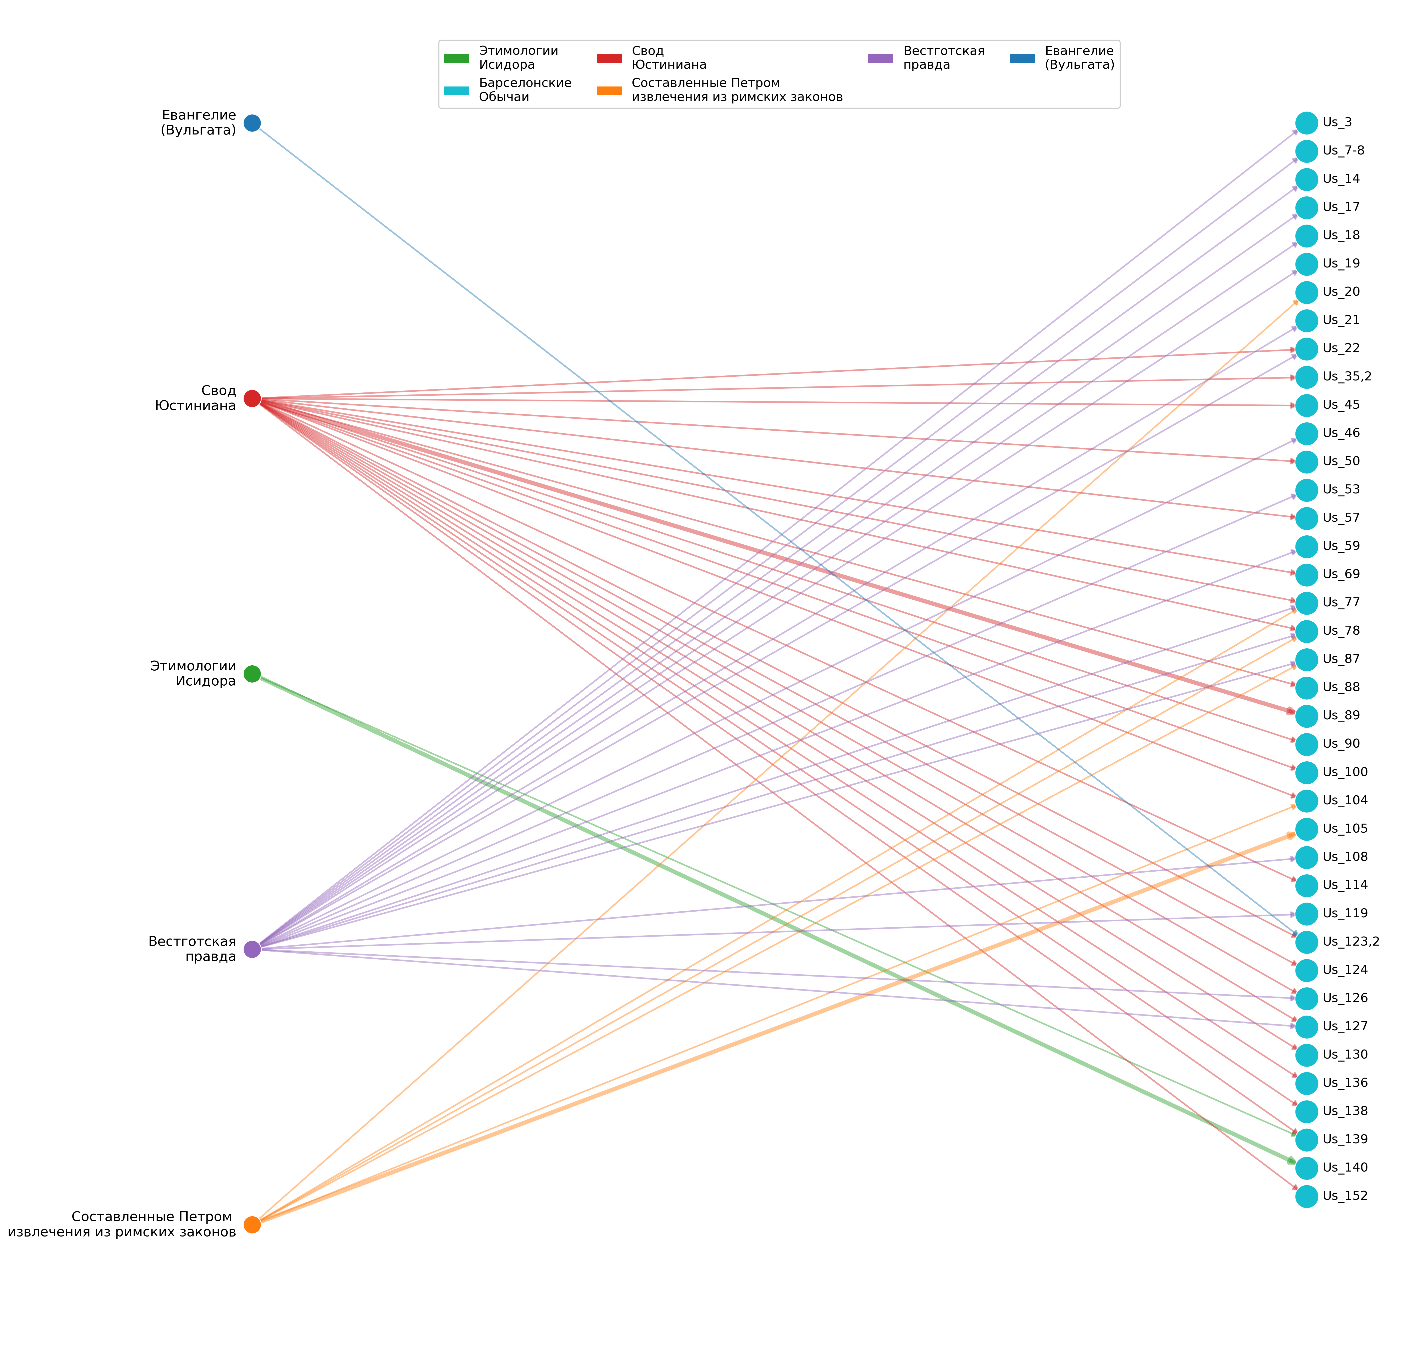
\includegraphics[width=0.95\textwidth]{Dissertation/images/korneeva/chapter1_01.png}
\caption{Граф выявленных текстуальных соответствий между латинскими источниками и отдельными статьями «Барселонских обычаев»}
\label{fig:chapter1-01}
\end{figure}

Граф демонстрирует выраженную асимметрию в распределении рёбер. Наиболее плотные пучки связей исходят от «Свода Юстиниана» и «Вестготской правды», что позволяет рассматривать их в качестве центральных латинских корпусов в данном эксперименте. При этом связи не распределены по всему массиву «Барселонских обычаев» равномерно --- они концентрируются вокруг ограниченного круга статей, среди которых особенно заметны статьи из начальной и средней части свода (в разное время включавшиеся исследователями в т.н. первоначальное ядро текста «Барселонских обычаев»\footnote{Подробнее об этой концепции в разделе «Источниковедение».}), а также несколько обычаев из его поздних слоёв. Уже на этом уровне граф подтверждает важное наблюдение: текстуальная близость между латинскими источниками и «Барселонскими обычаями» носит выборочный характер, концентрируясь вокруг конкретных статей и правовых норм.

Содержательное значение такой конфигурации особенно хорошо видно на материале сильнейших соответствий, зафиксированных в markdown-отчёте к данному эксперименту.

\begin{center}
\small
\setlength{\tabcolsep}{2pt}
% Метрики расположены по строкам: так таблица сохраняет 12-й кегль и
% полностью помещается на странице книжной ориентации.
\begin{longtable}{|p{0.22\textwidth}|p{0.24\textwidth}|p{0.24\textwidth}|p{0.24\textwidth}|}
\caption{Значения метрик и итоговое ранжирование трёх сильнейших соответствий латинских источников и «Барселонских обычаев»}\label{tab:ch1-latin-ranking}\\
\hline
\textbf{Показатель} & \textbf{\emph{Etymologiae} V.18 $\rightarrow$ Us. 140} & \textbf{Dig. 22.5.6 $\rightarrow$ Us. 89} & \textbf{\emph{Exceptiones legum Romanorum} IV.17 $\rightarrow$ Us. 105} \\ \hline
Косинусное сходство & 0,917 (1) & 0,692 (3) & 0,489 (4) \\ \hline
Tesserae & 4,566 (1) & 2,090 (5) & 2,779 (2) \\ \hline
Мягкое косинусное сходство & 0,929 (1) & 0,568 (6) & 0,703 (3) \\ \hline
Нормированное выравнивание & 1,727 (1) & 1,091 (2) & 0,798 (18) \\ \hline
Сумма рангов & 1+1+1+1=\textbf{4} & 3+5+6+2=\textbf{16} & 4+2+3+18=\textbf{27} \\ \hline
Парето-слой & 1 & 2 & 2 \\ \hline
Итоговая позиция & \textbf{1} & \textbf{2} & \textbf{3} \\ \hline
\end{longtable}
\end{center}

В скобках после значения каждой метрики указано место пары по соответствующему показателю. Сумма рангов рассчитывалась как сумма четырёх таких мест. Чем меньше полученное значение, тем более устойчиво пара занимает высокие позиции по совокупности применённых мер.

Наиболее сильное совпадение было выявлено между фрагментом из XVIII книги «Этимологий» Исидора Севильского, озаглавленным «О привилегиях», и 140-й статьёй «Барселонских обычаев». В обоих текстах содержится одна и та же дефиниция: привилегии определяются как \emph{«законы частных лиц»}, а происхождение самого термина объясняется его принадлежностью к сфере частного права.

\begin{center}
\small
\setlength{\tabcolsep}{2pt}
\begin{longtable}{|p{\dimexpr0.94\textwidth/3\relax}|p{\dimexpr0.94\textwidth/3\relax}|p{\dimexpr0.94\textwidth/3\relax}|}
\caption{Сопоставление текста \emph{Etymologiae} V.18 и статьи D2 (140) «Барселонских обычаев»}\label{tab:ch1-etymologiae}\\
\hline
\textbf{Элемент сопоставления} & \textbf{\emph{Etymologiae}}\textbf{ V.18} & \textbf{«Барселонские обычаи», }\textbf{ }\textbf{Us}\textbf{. D2 (140)} \\ \hline
\textbf{Итоговый редуцированный текст} & \emph{priuilegiis}\emph{ }\emph{priuilegia}\emph{ }\emph{sunt}\emph{ }\emph{leges}\emph{ }\emph{priuat}\emph{ }\emph{quasi}\emph{ }\emph{priu}\emph{ }\emph{leges}\emph{ }\emph{priuilegium}\emph{ }\emph{dictum}\emph{ }\emph{priuato}\emph{ }\emph{fera} & \emph{priuilegia}\emph{ sunt leges }\emph{priuat}\emph{ quasi }\emph{priuate}\emph{ leges }\emph{priuilegium}\emph{ dictum }\emph{priuato}\emph{ }\emph{fera} \\ \hline
\textbf{Текст по изданию} & \emph{De }\emph{privilegiis}\emph{. }\emph{Privilegia}\emph{ }\emph{autem}\emph{ }\emph{sunt}\emph{ }\emph{leges}\emph{ }\emph{privatorum}\emph{, }\emph{quasi}\emph{ }\emph{privatae}\emph{ }\emph{leges}\emph{. }\emph{Nam}\emph{ }\emph{privilegium}\emph{ }\emph{inde}\emph{ }\emph{dictum}\emph{, }\emph{quod}\emph{ in }\emph{privato}\emph{ }\emph{feratur}\footnote{\emph{Isidori}\emph{ }\emph{Hispalensis}\emph{ }\emph{Episcopi} Etymologiarum sive Originum libri XX. V.18 // Isidori Hispalensis Episcopi Etymologiarum sive Originum libri XX / rec. \emph{W.M.~Lindsay}. Oxonii: e Typographeo Clarendoniano, 1911. T.~1. P.~[207].}\emph{.} & \emph{Priuilegia}\emph{ }\emph{autem}\emph{ }\emph{sunt}\emph{ }\emph{leges}\emph{ }\emph{priuatorum}\emph{, }\emph{quasi}\emph{ }\emph{priuate}\emph{ }\emph{leges}\emph{; }\emph{nam}\emph{ }\emph{priuilegium}\emph{ }\emph{inde}\emph{ }\emph{dictum}\emph{, }\emph{quod}\emph{ in }\emph{priuato}\emph{ }\emph{feratur}\footnote{Usatges de Barcelona. Us. D2 (140). P.~173.}\emph{.} \\ \hline
\textbf{Перевод на русский язык} & \textbf{О привилегиях.} Привилегии --- это законы, установленные для частных лиц, как бы частные законы. Слово «привилегия» получило своё название оттого, что такой закон устанавливается в отношении частного лица. & Привилегии --- это законы, установленные для частных лиц, как бы частные законы; слово «привилегия» получило своё название оттого, что она устанавливается в отношении частного лица. \\ \hline
\end{longtable}
\end{center}

Это совпадение следует признать практически дословным: здесь совпадает не только общий смысл высказывания и не только набор отдельных юридических терминов, но и вся конструкция определения целиком. Именно этим объясняются и исключительно высокие показатели по всем метрикам: данная пара заняла первое место в ходе ранговой агрегации, вошла в первый слой парето-фильтрации и получила наилучшие показатели сходства по всем основным метрикам сравнения. Для историка права этот результат не является самостоятельным открытием, так как источник заимствования был установлен ещё Ж.~Бастардесом-и-Парерой\footnote{Usatges de Barcelona. Apéndix D.P.~172.}, однако требует внимательного рассмотрения в контексте текстуальной традиции.

Определение привилегии в 18-й главе V книги «Этимологий», вероятнее всего, было взято Исидором Севильским из глосс Плацида\footnote{\textbf{«}\textbf{Глоссы}\textbf{ }\textbf{Плацида}\textbf{»} (Glossae Placidi, или Placidus, Liber glossarum) --- латинский алфавитный глоссарий, традиционно приписываемый грамматику Плациду, которого иногда отождествляют с Лактанцием Плацидом. Личность составителя и время формирования сборника точно не установлены; обычно его относят к позднеантичной глоссографической традиции V--VI~вв. О заимствовании этой формулы Исидором Севильским см. \emph{Telaretti~E}\emph{. }I~presupposti e le fonti del diritto in Isidoro di Siviglia (Etymologiarum liber V, 1--21): tesi di dottorato. Palermo: Università degli Studi di Palermo, 2011. P.~217--218.}: \emph{«привилегии --- это законы, относящиеся к частным лицам, или пожалования, предоставляемые правителями»}\footnote{Формула о привилегиях в «Глоссах Плацида»: «privilegia leges privatorum seu beneficia quae a principibus conceduntur…» (\emph{Placidus}\emph{.} Liber glossarum. Glossaria reliqua. l. 25--27 // Corpus glossariorum Latinorum / ed. G.~Goetz. Lipsiae: in aedibus B.G.~Teubneri, 1894. Vol.~V.P.~94).}. Последующее собственно этимологическое пояснение Исидора Севильского \emph{«}\emph{…оттого, что такой закон устанавливается в отношении частного лица}\emph{»}\footnote{\emph{Isidori}\emph{ }\emph{Hispalensis}\emph{ }\emph{Episcopi} Etymologiarum sive Originum libri XX. V.18 // Isidori Hispalensis Episcopi Etymologiarum sive Originum libri XX / rec. \emph{W.M.~Lindsay}. Oxonii: e Typographeo Clarendoniano, 1911. T.~1. «…quod in privato feratur». P.~[207].} связано с более ранним римским пониманием привилегии как постановления, относящегося к отдельному лицу, известным по текстам Цицерона, Авла Геллия и Феста. Непосредственный источник этой части определения установить невозможно: вероятно, Исидор воспринял её через позднеантичную правовую традицию.

Таким образом, совпадение статьи 140 «Барселонских обычаев» с текстом Исидора следует рассматривать как воспроизведение формулы, уже имевшей длительную историю в латинской правовой традиции. При этом почти полное совпадение последовательности слов позволяет считать именно Исидора Севильского наиболее вероятным посредником. Использование в «Барселонских обычаях» авторитетного текста, принадлежащего не к узкоправовой, а к энциклопедической латинской (и шире --- Пиренейской) традиции свидетельствует о бытовании среди легистов-составителей правовой культуры, из которой заимствовались готовые формулы нормативного языка.

Второе место по силе в данном эксперименте занимает соответствие между фрагментом 22-й книги «Свода Юстиниана» и B6-й (89-й) статьёй «Барселонских обычаев».

\begin{center}
\small
\setlength{\tabcolsep}{2pt}
\begin{longtable}{|p{\dimexpr0.94\textwidth/3\relax}|p{\dimexpr0.94\textwidth/3\relax}|p{\dimexpr0.94\textwidth/3\relax}|}
\caption{Сопоставление текста \emph{Digesta} 22.5.6 и статьи B6 (89) «Барселонских обычаев»}\label{tab:ch1-digesta}\\
\hline
\textbf{Элемент сопоставления} & \textbf{\emph{Digesta}}\textbf{ 22.5.6} & \textbf{«Барселонские обычаи», }\textbf{ }\textbf{Us}\textbf{. B6 (89)} \\ \hline
\textbf{Итоговый редуцированный текст} & \emph{idon uident testes impera pot testes fia} & \emph{idon testes uident impera pot testes fia} \\ \hline
\textbf{Текст по изданию} & \emph{Idonei non videntur esse testes, quibus imperari potest ut testes fiant}\footnote{Digesta. 22.5.6 // Corpus iuris civilis. Vol.~1: Institutiones; Digesta / Institutiones recognovit P.~Krueger; Digesta recognovit Th.~Mommsen, retractavit P.~Krueger. Ed. stereotypa XV. Berolini: apud Weidmannos, 1928. P.~327.}\emph{.} & \emph{Idonei testes non uidentur esse quibus imperari potest ut testes fiant}\footnote{Usatges de Barcelona. Us. B6 (89). P.~170.}\emph{.} \\ \hline
\textbf{Перевод на русский язык} & Надлежащими свидетелями не считаются те, кому можно приказать выступить свидетелями. & Надлежащими свидетелями не считаются те, кому можно приказать выступить свидетелями. \\ \hline
\end{longtable}
\end{center}

Заключительная формула B6-й (89-й) статьи «Барселонских обычаев» восходит к фрагменту второй книги «Правил» римского правоведа Лициния Руфина\footnote{\textbf{Марк Гней }\textbf{Лициний}\textbf{ Руфин (M. }\textbf{Cn}\textbf{. }\textbf{Licinius}\textbf{ }\textbf{Rufinus}\textbf{)}\textbf{ }--- римский юрист и чиновник первой пол. III~в. Его не сохранившееся целиком сочинение «Правила» (Regulae) насчитывало двенадцать или тринадцать книг; семнадцать извлечений из него вошли в Дигесты Юстиниана. Рассматриваемая сентенция происходит из второй книги этого труда (Dig. 22.5.6). См.: \emph{Millar}\emph{ }\emph{F}\emph{.} The Greek East and Roman Law: The Dossier of M.Cn.~Licinius Rufinus // The Journal of Roman Studies. 1999. Vol.~89. P.~91--99; \emph{Lenel}\emph{ }\emph{O}\emph{.} Palingenesia Iuris Civilis: Iuris consultorum reliquiae quae Iustiniani Digestis continentur ceteraque iuris prudentiae civilis fragmenta minora secundum auctores et libros. Lipsiae: Bernhard Tauchnitz, 1889. Vol.~1. Col. 559--562.}, включённому в титул Дигест о свидетелях. Автоматическое сопоставление верно определило происхождение данного фрагмента из области римского права, однако само по себе оно ещё не может установить непосредственный источник, откуда эта формула попала в текст «Барселонских обычаев».

К концу XI в. --- началу XII~в. эта сентенция Лициния Руфина уже существовала вне полного текста Дигест и распространялась в составе канонических компиляций. Она представлена в «Британском собрании» (Collectio Britannica)\footnote{\emph{Conrat}\emph{ M. }Der Pandekten- und Institutionenauszug der brittischen Dekretalensammlung: Quelle des Ivo. Berlin: Weidmannsche Buchhandlung, 1887. S. 5--12.}, «Декрете» и «Панормии»\emph{ }Иво Шартрского\footnote{\emph{Ivo Carnotensis.} Decretum. XVI. 181 // Patrologiae cursus completus. Series Latina / accurante J.-P.~Migne. Parisiis: apud J.-P.~Migne editorem, 1855. T.~161. Col. 939; Idem. Panormia. V.33 // Ibid. Col. 1219.}. В этих канонических компиляциях окончание фразы передано в редакции «\emph{ut }\emph{testes}\emph{ }\textbf{\emph{sint}}\emph{»}, тогда как в Дигестах и статье «Барселонских обычаях» сохранился вариант «\emph{ut }\emph{testes}\emph{ }\textbf{\emph{fiant}}\emph{»}. Наличие формулы в догратиановских памятниках канонического права свидетельствует о том, что она могла быть известна составителю «Барселонских обычаев» без непосредственного обращения к полному тексту Дигест. Вместе с тем широкое распространение этой сентенции не позволяет по одному совпадению связать её попадание в текст B6-й (89-й) статьи «Барселонских обычаев» с какой-либо конкретной канонической компиляцией.

Более конкретную гипотезу о пути передачи текста предложил французский историк права А.~Гурон. Он обратил внимание, что эта же сентенция в формулировке «\emph{ut }\emph{testes}\emph{ }\textbf{\emph{fiant}}» находится в особом приложении к парижской рукописи «Тюбингенской книги»\footnote{\emph{Flach }\emph{J. }Études critiques sur l’histoire du droit romain au Moyen Âge, avec textes inédits. Paris: L. Larose et Forcel, 1890. P.~235; \emph{Gouron~A. }Sur la compilation des Usages de Barcelone au douzième siècle //\emph{ Idem. }Pionniers du droit occidental au Moyen Âge. Aldershot; Burlington: Ashgate Variorum, 2006. № V.P.~223--224.}. В непосредственной близости от неё в этой рукописи помещены определения для терминов \emph{furtum}, \emph{rapina} и \emph{invasio}, параллели которым также присутствуют в тексте «Барселонских обычаев». На основании совокупности этих совпадений А.~Гурон заключил, что составитель свода пользовался рукописью извлечений из Дигест, близкой к «Тюбингенской книге», хотя и не тождественной сохранившемуся парижскому списку\footnote{\textbf{«}\textbf{Тюбингенская}\textbf{ книга» }(Liber Tubingensis) --- принятое в историографии условное название анонимной компиляции римского права, сохранившейся в нескольких рукописях; название происходит от одного из её списков, хранящегося в Университетской библиотеке г.~Тюбинген. Памятник представляет собой собрание кратких извлечений и переработок норм римского права, предназначенное, по-видимому, для преподавания и практического применения. Согласно датировке А.~Гурона, сборник был составлен около середины XII~в. в Южной Франции. «Тюбингенская книга» принадлежит к тому же кругу южнофранцузских компиляций римского права, что «Ашбернемская книга» и «Грацская книга». Материал этих трёх сборников был позднее использован в «Составленных Петром извлечениях из Римских законов». Подробнее см. \emph{Gouron A.} Sur la patrie et la datation du «Livre de Tubingue» et des «Exceptiones Petri» // Rivista internazionale di diritto comune. 2003. Vol.~14. P.~15--39; \emph{Idem.} Sur la compilation des Usages de Barcelone au douzième siècle // \emph{Idem.} Pionniers du droit occidental au Moyen Âge. Aldershot; Burlington: Ashgate Variorum, 2006. № V.P.~223--224.}.

Третье по значимости совпадение связывает фрагмент из «Составленных Петром извлечений из римских законов» с 80-й (105-й) статьёй «Барселонских обычаев».

\begin{center}
\small
\setlength{\tabcolsep}{2pt}
\begin{longtable}{|p{\dimexpr0.94\textwidth/3\relax}|p{\dimexpr0.94\textwidth/3\relax}|p{\dimexpr0.94\textwidth/3\relax}|}
\caption{Сопоставление текста «Составленные Петром извлечения из римских законов» IV.17 и статьи 80 (105) «Барселонских обычаев»}\label{tab:ch1-petri-exceptiones}\\
\hline
\textbf{Элемент сопоставления} & \textbf{\emph{«Составленные Петром извлечения из римских законов»,}}\textbf{ IV.17} & \textbf{«Барселонские обычаи», }\textbf{Us}\textbf{.}\textbf{ 80}\textbf{ }\textbf{(}\textbf{105}\textbf{)} \\ \hline
\textbf{Итоговый редуцированный текст} & \emph{aduers}\emph{ }\emph{alium}\emph{ }\emph{aliqu}\emph{ }\emph{actionem}\emph{ }\emph{habuer}\emph{ }\emph{iusti}\emph{с}\emph{ }\emph{faciend}\emph{ }\emph{uocauer}\emph{ }\emph{timo}\emph{ }\emph{dei}\emph{ }\emph{iussu}\emph{ }\emph{iudicis}\emph{ }\emph{propinquo}\emph{ }\emph{amico}\emph{ c}\emph{o}\emph{monitu}\emph{ }\emph{iustic}\emph{ }\emph{acto}\emph{ }\emph{face}\emph{ }\emph{uoluer}\emph{ }\emph{actor}\emph{ }\emph{ira}\emph{ }\emph{co}\emph{mmo}\emph{ts}\emph{ }\emph{res}\emph{ }\emph{mobil}\emph{ }\emph{rapuer}\emph{ }\emph{immobiles}\emph{ }\emph{inuaser}\emph{ }\emph{domos}\emph{ c }\emph{cremaner}\emph{ }\emph{uineas}\emph{ }\emph{mes}\emph{ }\emph{ses}\emph{ }\emph{arbor}\emph{ }\emph{deuastauer}\emph{ }\emph{posteaq}\emph{ }\emph{reus}\emph{ }\emph{aliquo}\emph{ }\emph{tem}\emph{ }\emph{iusti}\emph{ }\emph{ciam}\emph{ }\emph{uener}\emph{ }\emph{quicquid}\emph{ }\emph{damni}\emph{ }\emph{acto}\emph{ }\emph{foec}\emph{ }\emph{luer}\emph{ }\emph{rebus}\emph{ }\emph{siris}\emph{ }\emph{poss}\emph{ }\emph{cepisse}\emph{ }\emph{primis}\emph{ }\emph{restitunt}\emph{ }\emph{postea}\emph{ }\emph{actor}\emph{ }\emph{ret}\emph{ }\emph{quas}\emph{ }\emph{bonis}\emph{ }\emph{possed}\emph{ }\emph{restituat}\emph{ }\emph{consumptum}\emph{ }\emph{uero}\emph{ d }\emph{iuc}\emph{ }\emph{presens}\emph{ }\emph{hab}\emph{ }\emph{restaur} & \emph{contra}\emph{ }\emph{alium}\emph{ }\emph{aliqu}\emph{ }\emph{querel}\emph{ }\emph{habuer}\emph{ }\emph{iustic}\emph{ }\emph{faciend}\emph{ }\emph{eum}\emph{ }\emph{uocauer}\emph{ }\emph{timo}\emph{ }\emph{dei}\emph{ }\emph{iudicis}\emph{ }\emph{iussu}\emph{ }\emph{propinqu}\emph{o}\emph{ }\emph{amic}\emph{ }\emph{commonitu}\emph{ }\emph{iustic}\emph{ }\emph{querelato}\emph{ }\emph{face}\emph{ }\emph{noluer}\emph{ }\emph{querel}\emph{ }\emph{ira}\emph{ }\emph{commot}\emph{ }\emph{res}\emph{ }\emph{mobil}\emph{ }\emph{rapuer}\emph{ }\emph{immobiles}\emph{ }\emph{inuaser}\emph{ }\emph{domos}\emph{ }\emph{concremauerit}\emph{ }\emph{messes}\emph{ }\emph{uineas}\emph{ }\emph{arbor}\emph{ }\emph{deuastauer}\emph{ }\emph{postea}\emph{ }\emph{reus}\emph{ }\emph{aliquo}\emph{ }\emph{tempo}\emph{ }\emph{iusticiam}\emph{ }\emph{uener}\emph{ }\emph{quicquid}\emph{ }\emph{dampni}\emph{ }\emph{querelator}\emph{ }\emph{fec}\emph{ }\emph{lucrum}\emph{ }\emph{poss}\emph{ }\emph{rebus}\emph{ }\emph{suis}\emph{ }\emph{cepisse}\emph{ }\emph{primum}\emph{ }\emph{restituat}\emph{ }\emph{postea}\emph{ }\emph{querel}\emph{ }\emph{res}\emph{ }\emph{quas}\emph{ }\emph{bonis}\emph{ }\emph{possidet}\emph{ }\emph{redd}\emph{ }\emph{consumpta}\emph{ }\emph{uero}\emph{ }\emph{aliquid}\emph{ }\emph{luc}\emph{ }\emph{presens}\emph{ }\emph{hab}\emph{ }\emph{tantum}\emph{ }\emph{restaur}\emph{ }\emph{postea}\emph{ }\emph{reus}\emph{ }\emph{iustic}\emph{ }\emph{faci}\emph{ }\emph{querelato}\emph{ }\emph{sicut}\emph{ }\emph{face}\emph{ }\emph{debuer}\emph{ }\emph{dec} \\ \hline
\textbf{Текст по изданию} & \emph{Si}\emph{ }\emph{quis}\emph{ }\emph{adversus}\emph{ }\emph{alium}\emph{ }\emph{aliquam}\emph{ }\emph{actionem}\emph{ }\emph{habuerit}\emph{ }\emph{et}\emph{ }\emph{ad}\emph{ }\emph{iustitiam}\emph{ }\emph{faciendam}\emph{ }\emph{vocaverit}\emph{, }\emph{ille}\emph{ }\emph{autem}\emph{ }\emph{nec}\emph{ }\emph{timore}\emph{ Dei, }\emph{nec}\emph{ }\emph{iussu}\emph{ }\emph{iudicis}\emph{, }\emph{nec}\emph{ }\emph{propinquorum}\emph{ }\emph{vel}\emph{ }\emph{amicorum}\emph{ }\emph{commonitu}\emph{ }\emph{iustitiam}\emph{ }\emph{actori}\emph{ }\emph{facere}\emph{ }\emph{voluerit}\emph{, }\emph{actor}\emph{ }\emph{autem}\emph{ }\emph{ira}\emph{ }\emph{commotus}\emph{ }\emph{res}\emph{ }\emph{eius}\emph{ }\emph{mobiles}\emph{ }\emph{rapuerit}\emph{, }\emph{immobiles}\emph{ }\emph{invaserit}\emph{, }\emph{domos}\emph{ }\emph{concremaverit}\emph{, }\emph{vineas}\emph{, }\emph{messes}\emph{ }\emph{et}\emph{ }\emph{arbores}\emph{ }\emph{devastaverit}\emph{, }\emph{posteaque}\emph{ }\emph{reus}\emph{ }\emph{aliquo}\emph{ }\emph{tempore}\emph{ }\emph{ad}\emph{ }\emph{iustitiam}\emph{ }\emph{venerit}\emph{, }\emph{quidquid}\emph{ }\emph{damni}\emph{ }\emph{actori}\emph{ }\emph{fecit}\emph{ }\emph{vel}\emph{ }\emph{lucrum}\emph{ }\emph{quod}\emph{ de }\emph{rebus}\emph{ }\emph{suis}\emph{ }\emph{posset}\emph{ }\emph{cepisse}\emph{, in }\emph{primis}\emph{ }\emph{ei}\emph{ }\emph{restituat}\emph{. }\emph{Postea}\emph{ }\emph{actor}\emph{ }\emph{res}\emph{ }\emph{quas}\emph{ }\emph{ex}\emph{ }\emph{bonis}\emph{ }\emph{eius}\emph{ }\emph{possedit}\emph{ }\emph{restituat}\emph{; }\emph{consumptarum}\emph{ }\emph{vero}\emph{ }\emph{si}\emph{ }\emph{quid}\emph{ }\emph{lucri}\emph{ }\emph{ad}\emph{ }\emph{praesens}\emph{ }\emph{habet}\emph{, }\emph{tamen}\emph{ }\emph{restauret}\emph{.} & \emph{Si}\emph{ }\emph{quis}\emph{ }\emph{contra}\emph{ }\emph{alium}\emph{ }\emph{aliquam}\emph{ }\emph{querelam}\emph{ }\emph{habuerit}\emph{ }\emph{et}\emph{ }\emph{ad}\emph{ }\emph{iusticiam}\emph{ }\emph{faciendam}\emph{ }\emph{eum}\emph{ }\emph{uocauerit}\emph{, }\emph{ille}\emph{ }\emph{autem}\emph{ }\emph{nec}\emph{ }\emph{timore}\emph{ Dei, }\emph{nec}\emph{ }\emph{iudicis}\emph{ }\emph{iussu}\emph{, }\emph{nec}\emph{ }\emph{propinquorum}\emph{ }\emph{uel}\emph{ }\emph{amicorum}\emph{ }\emph{commonitu}\emph{ }\emph{iusticiam}\emph{ }\emph{querelatori}\emph{ }\emph{facere}\emph{ }\emph{noluerit}\emph{; }\emph{querelator}\emph{ }\emph{autem}\emph{, }\emph{ira}\emph{ }\emph{commotus}\emph{, }\emph{res}\emph{ }\emph{eius}\emph{ }\emph{mobiles}\emph{ }\emph{rapuerit}\emph{, }\emph{immobiles}\emph{ }\emph{inuaserit}\emph{, }\emph{domos}\emph{ }\emph{concremauerit}\emph{, }\emph{messes}\emph{ }\emph{et}\emph{ }\emph{uineas}\emph{ }\emph{et}\emph{ }\emph{arbores}\emph{ }\emph{deuastauerit}\emph{; }\emph{posteaque}\emph{ }\emph{reus}\emph{ }\emph{aliquo}\emph{ }\emph{tempore}\emph{ }\emph{ad}\emph{ }\emph{iusticiam}\emph{ }\emph{uenerit}\emph{; }\emph{quicquid}\emph{ }\emph{dampni}\emph{ }\emph{ad}\emph{ }\emph{querelatorem}\emph{ }\emph{fecit}\emph{ }\emph{uel}\emph{ }\emph{lucrum}\emph{ }\emph{quod}\emph{ }\emph{posset}\emph{ de }\emph{rebus}\emph{ }\emph{suis}\emph{ }\emph{cepisse}\emph{, }\emph{primum}\emph{ }\emph{ei}\emph{ }\emph{restituat}\emph{, }\emph{et}\emph{ }\emph{postea}\emph{ }\emph{querelator}\emph{ }\emph{res}\emph{ }\emph{quas}\emph{ }\emph{ex}\emph{ }\emph{bonis}\emph{ }\emph{eius}\emph{ }\emph{possidet}\emph{ }\emph{ei}\emph{ }\emph{reddat}\emph{; }\emph{consumpta}\emph{ }\emph{uero}\emph{, }\emph{si}\emph{ }\emph{aliquid}\emph{ }\emph{lucri}\emph{ }\emph{ad}\emph{ }\emph{presens}\emph{ }\emph{habet}\emph{ }\emph{tantum}\emph{ }\emph{restauret}\emph{, }\emph{et}\emph{ }\emph{postea}\emph{ }\emph{reus}\emph{ }\emph{iusticiam}\emph{ }\emph{faciat}\emph{ }\emph{querelatori}\emph{ }\emph{sicut}\emph{ }\emph{facere}\emph{ }\emph{debuerit}\emph{ }\emph{et}\emph{ }\emph{decet}\emph{.} \\ \hline
\textbf{Перевод на русский язык} & Если кто-либо имеет к другому какое-либо притязание и вызовет его для правосудия, а тот ни из страха Божия, ни по приказу судьи, ни по увещеванию родственников или друзей не пожелает удовлетворить требование истца по праву; истец же, разгневанный, захватит его движимое имущество, завладеет недвижимым, сожжёт дома, опустошит виноградники, посевы и деревья, а затем ответчик когда-либо явится для осуществления правосудия, то прежде всего он должен возместить истцу весь причинённый ущерб либо выгоду, которую тот мог бы получить от своего имущества. После этого истец должен возвратить вещи, которыми завладел из имущества ответчика; что же касается потреблённого, то он должен возместить лишь ту выгоду, которую всё ещё имеет от него. & Если кто-либо имеет к другому какое-либо притязание и вызовет его для правосудия, а тот ни из страха Божия, ни по приказу судьи, ни по увещеванию родственников или друзей не пожелает удовлетворить требование заявителя по праву; заявитель же, разгневанный, захватит его движимое имущество, завладеет недвижимым, сожжёт дома, опустошит посевы, виноградники и деревья, а затем ответчик когда-либо явится для осуществления правосудия, то прежде всего он должен возместить заявителю весь причинённый ущерб либо выгоду, которую тот мог бы получить от своего имущества. После этого заявитель должен возвратить вещи, которыми завладел из имущества ответчика; что же касается потреблённого, то он должен возместить лишь ту выгоду, которую всё ещё имеет от него. \\ \hline
\end{longtable}
\end{center}

Соответствие между главой 17 книги IV «Составленных Петром извлечений из римских законов» и 105 статьёй «Барселонских обычаев» требует уточнения с учётом рукописной традиции. В критическом издании К.Г.~Мора 105-я статья «Барселонских обычаев» сопоставлена с 14-й главой «Тюбингенской книги» и 18-й главой «Составленных Петром извлечений из римских законов»\footnote{\emph{Mor~C.G. }En torno a la formación del texto de los Usatici Barchinonae // Anuario de Historia del Derecho Español. 1957--1958. T.~27--28. P.~432, 434--435.}. К.Г.~Мор рассматривал 105-ю статью «Барселонских обычаев» как прямое заимствование из «Тюбингенской книги», однако А.~Гурон показал, что соответствующий фрагмент передан в ней и в «Составленных Петром извлечений из римских законов» в одинаковой редакции\footnote{\emph{Gouron~A. }Sur la compilation des Usages de Barcelone au douzième siècle // \emph{Gouron}\emph{~}\emph{A. }Pionniers du droit occidental au Moyen Âge. Aldershot; Burlington: Ashgate Variorum, 2006. P.~223--224.}. Поэтому одно только текстуальное совпадение не позволяет выбрать между этими двумя потенциальными источниками.

Общий для «Тюбингенской книги» и «Составленных Петром извлечений из римских законов» текст представляет собой развёрнутое рассуждение об отказе ответчика исполнить требование истца и последующее самоуправство истца с последующей взаимной реституцией сторон. Помимо приказа судьи в качестве мотивации для отказа от самоуправства упомянуты страх Божий и увещание близких. Действия истца не признаются правомерными: отказ ответчика не освобождает его от обязанности вернуть захваченное.

Вся структура этой нормы сохраняется в 105-й статье «Барселонских обычаев» с некоторыми лексическими заменами, которые мы рассмотрим подробнее. Так, термины actio и actor заменены словами querela и querelator, обозначающими соответственно жалобу или притязание и лицо, которое его предъявляет. Формула adversus alium заменена на contra alium, in primis --- на primum, а при описании возврата имущества вместо повторного restituat употреблён глагол reddat. Эти изменения не затрагивают основного содержания нормы, однако отражаются на результатах количественного анализа совпадений, увеличивая сумму рангов для данной пары соответствий.

Особого внимания заслуживает чтение noluerit в  105-й статье «Барселонских обычаев»\footnote{Usatges de Barcelona. Us. 80 (105). P.~118.}. В издании Савиньи в соответствующем месте «Составленные Петром извлечения из римских законов» встречаем уже voluerit, несмотря на заголовок главы\footnote{Petri Exceptiones legum Romanorum. Lib. IV. Cap. 17 //\emph{ Savigny F.C. von.} Geschichte des römischen Rechts im Mittelalter. 2. Aufl. Bd. 2. Heidelberg: J.\emph{C.B.~Mohr}, 1834. Anhang I.A: «De his, qui iustitiam facere noluerint». S. 410.}, и дальнейшая логика нормы предполагает именно отказ ответчика. Обращение к «Барселонским обычаям» восстанавливает смысловую связь между отказом от правосудия и последующим самоуправством истца. Оно могло возникнуть в результате редакторского исправления, однако нельзя исключать, что составитель располагал списком, уже содержавшим отрицательную форму. Без учёта вариантов рукописей «Тюбингенской книги» и «Составленных Петром извлечений из римских законов» это различие не может служить основанием для определения непосредственного источника.

Следовательно, статья 105 не является механической вставкой текста из источника-посредника. Составители «Барселонских обычаев» уточнили обозначения участников, исправили или воспроизвели более логичный вариант глагола в начале нормы noluerit и дополнили её заключительным предписанием об исполнении первоначальной обязанности. Результат вычислительного сопоставления в данном случае выявляет общий текстовый пласт «Тюбингенской книги» и «Составленных Петром извлечений из римских законов».

Для определения наиболее вероятного посредника необходимо учитывать всю совокупность заимствованных в «Барселонские обычаи» фрагментов из «Составленных Петром извлечений из римских законов», а именно тексты статей 77, 89 и 169. По предположению А.~Гурона, составитель «Барселонских обычаев» пользовался не сохранившимся до наших дней списком, который сохранял структуру «Тюбингенской книги», но уже включал отдельные чтения, известные по «Составленным Петром извлечениям из римских законов». С учётом данных количественного анализа соответствий такая гипотеза представляется нам весьма обоснованной.

Наряду с основным графом важную интерпретационную роль играет и двумерная схема парето-слоёв.

\begin{figure}[htbp]
\centering
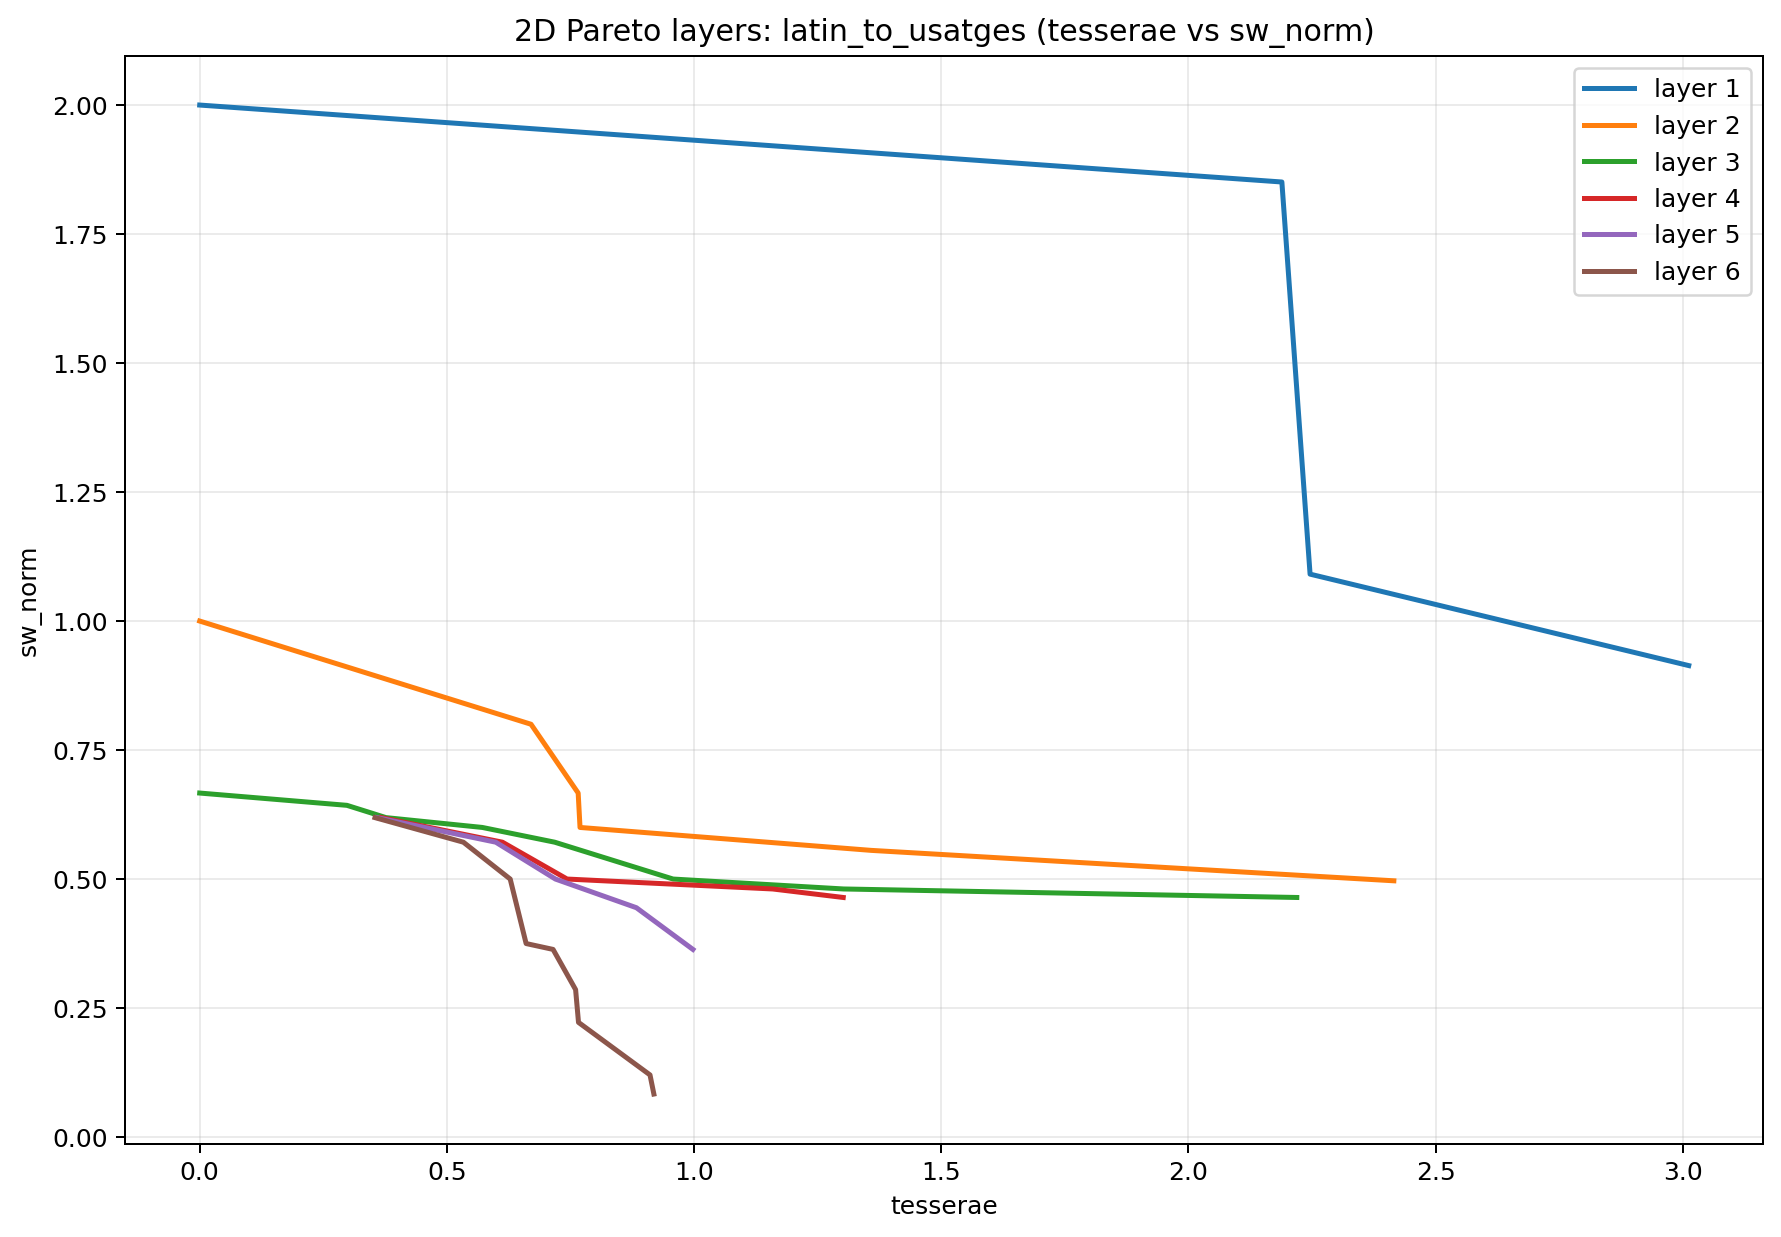
\includegraphics[width=0.95\textwidth]{Dissertation/images/korneeva/chapter1_02.png}
\caption{Двумерные парето-слои для эксперимента «латинские источники $\rightarrow$ Барселонские обычаи» в пространстве мер Tesserae и $\operatorname{SW}_{\mathrm{norm}}$}
\label{fig:chapter1-02}
\end{figure}

Данный рисунок показывает, каким образом результаты распределяются в пространстве двух параметров --- пересечения по редкой лексике и силе локального выравнивания. Первый слой формирует верхнюю оболочку множества результатов и включает те пары, которые оказываются недоминируемыми одновременно по обоим показателям. Методологически это означает, что в данном эксперименте сохраняются не только пары с наибольшим словарным пересечением, но и случаи, где особенно сильно проявлено именно локальное структурное совпадение. Текстуальная связь между латинским источником и отдельными статьями «Барселонских обычаев» свода может быть значимой либо как почти буквальное локальное воспроизведение пассажа. Если бы отбор строился по одной линейной шкале, часть таких случаев оказалась бы вытесненной более «усреднёнными» парами. На схеме же видно, что первый и второй слои занимают достаточно широкое пространство, а значит, отбор не схлопывается в единственный тип соответствий.

В отношении сопоставления с качественными историко-правовыми исследованиями результаты данного эксперимента в целом согласуются с представлением о том, что «Барселонские обычаи» формировались в постоянном контакте с латинской юридической традицией, прежде всего с римским правом. Однако вычислительный анализ позволяет перевести это общее положение в более точную форму: он показывает, какие именно обычаи демонстрируют такую связь, насколько она интенсивна и какого типа совпадения лежат в её основе.

\subsection{«Барселонские обычаи» и другие каталонские сборники обычного права}

Второй эксперимент был посвящён сопоставлению «Барселонских обычаев» с другими каталонскими сборниками обычного права. В отличие от предыдущего случая, данный правовой памятник теперь выступал как отправная точка сравнения, а на противоположной стороне расположены статьи «Обычаев Тортосы» (9-я книга)\footnote{В данном случае, намеренное ограничение объёма текста источника обоснованно языковым строем, именно на 9-ю книгу «Обычаев Тортосы» приходится наибольшее число латиноязычных вставок и цитирований. Подробнее об этом, см. \emph{Корнеева А.Д.}~Классификация латинских заимствований и цитат в тексте Обычаев Тортосы: количественный и качественный аспекты // Человеческий капитал. 2023. №~10(178). С.~31--40.}, «Обычаев Льейды», «Обычаев Миравета», «Обычаев Орты», привилегии «Обычаев Тарреги» и «Кутюмов Перпиньяна». Итоговый граф имеет существенно иную структуру, чем в эксперименте с латинскими источниками: он отражает внутреннюю сеть связей внутри каталонской правовой традиции.

\begin{figure}[htbp]
\centering
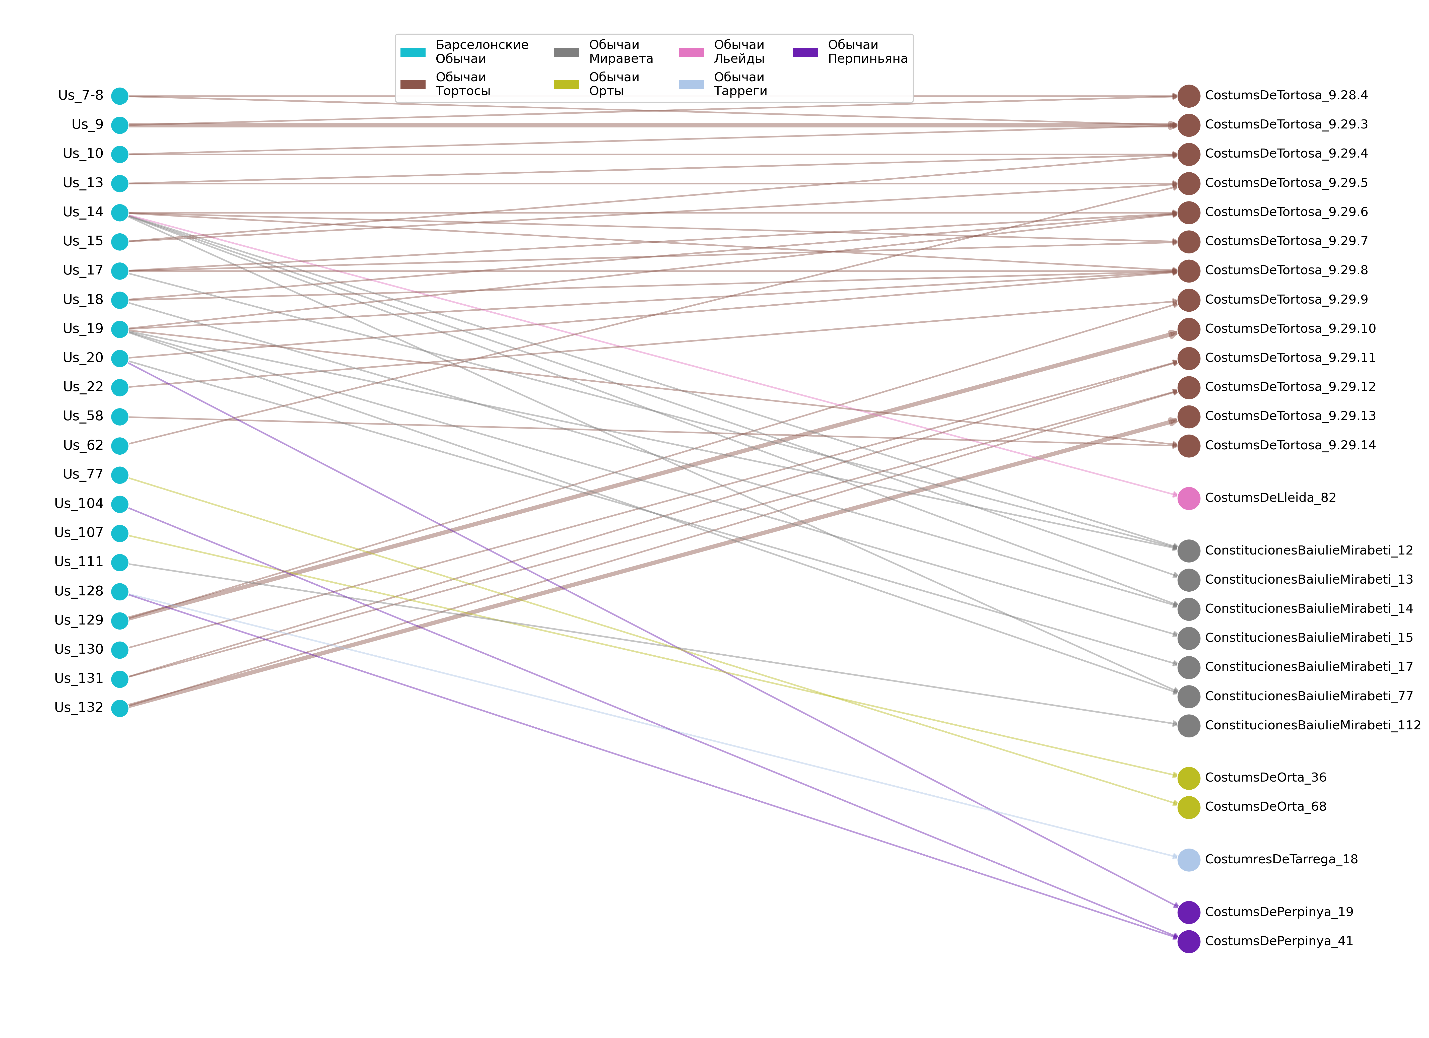
\includegraphics[width=0.95\textwidth]{Dissertation/images/korneeva/chapter1_03.png}
\caption{Граф текстуальных связей между «Барселонскими обычаями» и другими каталонскими сборниками обычного права}
\label{fig:chapter1-03}
\end{figure}

Наиболее заметная особенность графа состоит в концентрации связей вокруг норм книги IX «Обычаев Тортосы». К этому корпусу ведёт большинство из 50 рёбер, сохранённых после парето-фильтрации, ранжирования и итогового отбора. Доминирование «Обычаев Тортосы» проявляется, таким образом, прежде всего в \textbf{числе высокоранжированных соответствий}, а не только в визуальной плотности линий. Дополнительным показателем служит то, что все три связи, выделенные увеличенной толщиной, соединяют статьи «Барселонских обычаев» именно с нормами IX.29.13, IX.29.10 и IX.29.3 «Обычаев Тортосы». Эти линии соответствуют трём первым позициям итогового ранжирования; их толщина не обозначает отдельного численного порога, а служит графическим маркером трёх сильнейших пар во всём отобранном множестве. Остальные рёбра, независимо от конкретных значений метрик и корпуса назначения, показаны одинаково тонкими линиями. Поэтому граф позволяет различить два самостоятельных признака --- количественное преобладание связей с «Обычаями Тортосы» и принадлежность трёх наиболее высоко ранжированных соответствий к тому же корпусу.

\begin{center}
\small
\setlength{\tabcolsep}{2pt}
\begin{longtable}{|p{0.22\textwidth}|p{0.24\textwidth}|p{0.24\textwidth}|p{0.24\textwidth}|}
\caption{Пары текстуальных совпадений «Барселонских обычаев» и «Обычаев Тортосы»}\label{tab:ch1-tortosa-pairs}\\
\hline
\textbf{Показатель} & \textbf{Us. 132 $\rightarrow$ \emph{Costums de Tortosa} IX.29.13} & \textbf{Us. 129 $\rightarrow$ \emph{Costums de Tortosa} IX.29.10} & \textbf{Us. 9 $\rightarrow$ \emph{Costums de Tortosa} IX.29.3} \\ \hline
Косинусное сходство & 0,836 (1) & 0,717 (6) & 0,762 (2) \\ \hline
Tesserae & 3,172 (4) & 3,573 (2) & 2,890 (7) \\ \hline
Мягкое косинусное сходство & 0,891 (2) & 0,779 (7) & 0,814 (5) \\ \hline
Нормированное выравнивание & 1,467 (8) & 1,710 (1) & 1,688 (2) \\ \hline
Сумма рангов & 1+4+2+8=\textbf{15} & 6+2+7+1=\textbf{16} & 2+7+5+2=\textbf{16} \\ \hline
Парето-слой & 1 & 1 & 1 \\ \hline
Итоговая позиция & \textbf{1} & \textbf{2} & \textbf{3} \\ \hline
\end{longtable}
\end{center}

Markdown-отчёт по данному эксперименту позволяет конкретизировать эту картину на уровне отдельных пар:

\begin{center}
\small
\setlength{\tabcolsep}{2pt}
\begin{longtable}{|p{\dimexpr0.94\textwidth/3\relax}|p{\dimexpr0.94\textwidth/3\relax}|p{\dimexpr0.94\textwidth/3\relax}|}
\caption{Сопоставление статьи 132 «Барселонских обычаев» и статьи IX.29.13 «Обычаев Тортосы»}\label{tab:ch1-tortosa-132}\\
\hline
\textbf{Элемент сопоставления} & \textbf{«Барселонские обычаи», }\textbf{ }\textbf{Us}\textbf{. }\textbf{111 (}\textbf{132}\textbf{)} & \textbf{«Обычаи Тортосы», IX.29.13} \\ \hline
\textbf{Итоговый редуцированный текст} & \emph{constituerunt}\emph{ }\emph{igi}\emph{ }\emph{quis}\emph{ }\emph{aliquo}\emph{ }\emph{ier}\emph{ }\emph{fuer}\emph{ }\emph{uia}\emph{ }\emph{domo}\emph{ }\emph{agro}\emph{ }\emph{seu}\emph{ }\emph{alio}\emph{ }\emph{quolibet}\emph{ }\emph{loco}\emph{ }\emph{aliqu}\emph{ }\emph{eum}\emph{ }\emph{requisierit}\emph{ }\emph{aliquid}\emph{ }\emph{tolle}\emph{ }\emph{uoluer}\emph{ }\emph{adiu}\emph{ }\emph{uet}\emph{ }\emph{eum}\emph{ }\emph{prout}\emph{ }\emph{melius}\emph{ }\emph{poss}\emph{ }\emph{engan}\emph{ }\emph{contra}\emph{ }\emph{cunctos}\emph{ }\emph{eciam}\emph{ }\emph{contra}\emph{ }\emph{senior}\emph{ }\emph{suos}\emph{ }\emph{nullam}\emph{ }\emph{pertimesc}\emph{ }\emph{calumpniam}\emph{ }\emph{senior}\emph{ }\emph{suus}\emph{ }\emph{nullo}\emph{ }\emph{modo}\emph{ }\emph{poss} & \emph{constituerunt}\emph{ }\emph{igi}\emph{ }\emph{quis}\emph{ }\emph{alio}\emph{ }\emph{ier}\emph{ }\emph{fuer}\emph{ }\emph{uia}\emph{ }\emph{domo}\emph{ }\emph{agro}\emph{ }\emph{seu}\emph{ }\emph{alio}\emph{ }\emph{quolibet}\emph{ }\emph{loco}\emph{ }\emph{aliqu}\emph{ }\emph{eum}\emph{ }\emph{requisierit}\emph{ }\emph{aliquid}\emph{ }\emph{desuo}\emph{ }\emph{tolle}\emph{ }\emph{uoluer}\emph{ }\emph{adiuu}\emph{ }\emph{eum}\emph{ }\emph{prout}\emph{ }\emph{melius}\emph{ }\emph{poss}\emph{ }\emph{enganno}\emph{ }\emph{contra}\emph{ }\emph{cunctos}\emph{ }\emph{contra}\emph{ }\emph{senior}\emph{ }\emph{suos}\emph{ }\emph{nullam}\emph{ }\emph{pertimesc}\emph{ }\emph{calumpniam}\emph{ }\emph{senior}\emph{ }\emph{suus}\emph{ }\emph{nullo}\emph{ }\emph{modo}\emph{ }\emph{poss}\emph{ }\emph{eum}\emph{ }\emph{suos}\emph{ }\emph{nullam}\emph{ }\emph{pertimesc}\emph{ }\emph{calumpniam}\emph{ }\emph{senior}\emph{ }\emph{suus}\emph{ }\emph{nullo}\emph{ }\emph{modo}\emph{ }\emph{poss} \\ \hline
\textbf{Текст по изданию} & \emph{Constituerunt}\emph{ }\emph{igitur}\emph{ ut }\emph{si}\emph{ }\emph{quis}\emph{ }\emph{cum}\emph{ }\emph{aliquo}\emph{ }\emph{ierit}\emph{ }\emph{uel}\emph{ }\emph{fuerit}\emph{, }\emph{siue}\emph{ in }\emph{uia}\emph{, }\emph{aut}\emph{ in }\emph{domo}\emph{, }\emph{siue}\emph{ in }\emph{agro}\emph{, }\emph{seu}\emph{ in }\emph{alio}\emph{ }\emph{quolibet}\emph{ }\emph{loco}\emph{, }\emph{si}\emph{ }\emph{aliquis}\emph{ }\emph{inde}\emph{ }\emph{eum}\emph{ }\emph{requisierit}\emph{ }\emph{uel}\emph{ }\emph{aliquid}\emph{ de }\emph{suo}\emph{ }\emph{ei}\emph{ }\emph{tollere}\emph{ }\emph{uoluerit}\emph{, }\emph{adiuuet}\emph{ }\emph{eum}\emph{ }\emph{prout}\emph{ }\emph{melius}\emph{ }\emph{possit}\emph{ }\emph{sine}\emph{ }\emph{engan}\emph{ }\emph{contra}\emph{ }\emph{cunctos}\emph{ }\emph{eciam}\emph{ }\emph{contra}\emph{ }\emph{seniores}\emph{ }\emph{suos}\emph{; }\emph{et}\emph{ }\emph{nullam}\emph{ }\emph{ex}\emph{ }\emph{hoc}\emph{ }\emph{pertimescat}\emph{ }\emph{calumpniam}\emph{, }\emph{et}\emph{ }\emph{senior}\emph{ }\emph{suus}\emph{ }\emph{nullo}\emph{ }\emph{modo}\emph{ }\emph{possit}\emph{ }\emph{eum}\emph{ }\emph{reptare}\emph{ }\emph{inde}\emph{ in }\emph{aliquo}\emph{ de }\emph{ominiatico}\emph{ }\emph{neque}\emph{ de }\emph{sacramento}\emph{ }\emph{transgresso}\footnote{Usatges de Barcelona. Us. 111(132). P.~144.}\emph{.} & \emph{Constituerunt}\emph{ }\emph{igitur}\emph{, ut }\emph{si}\emph{ }\emph{quis}\emph{ }\emph{cum}\emph{ }\emph{alio}\emph{ }\emph{ierit}\emph{ }\emph{vel}\emph{ }\emph{fuerit}\emph{ }\emph{sive}\emph{ in }\emph{via}\emph{ }\emph{sive}\emph{ in }\emph{domo}\emph{, }\emph{sive}\emph{ in }\emph{agro}\emph{, }\emph{seu}\emph{ in }\emph{alio}\emph{ }\emph{quolibet}\emph{ }\emph{loco}\emph{, }\emph{si}\emph{ }\emph{aliquis}\emph{ }\emph{eum}\emph{ }\emph{requisierit}\emph{, }\emph{vel}\emph{ }\emph{aliquid}\emph{ de }\emph{suo}\emph{ }\emph{tollere}\emph{ }\emph{voluerit}\emph{, }\emph{adiuvet}\emph{ }\emph{eum}\emph{ }\emph{inde}\emph{ }\emph{prout}\emph{ }\emph{melius}\emph{ }\emph{possit}\emph{, }\emph{sine}\emph{ }\emph{enganno}\emph{ }\emph{contra}\emph{ }\emph{cunctos}\emph{ }\emph{et}\emph{ }\emph{contra}\emph{ }\emph{seniores}\emph{ }\emph{suos}\emph{; }\emph{et}\emph{ }\emph{nullam}\emph{ }\emph{ex}\emph{ }\emph{hoc}\emph{ }\emph{pertimescat}\emph{ }\emph{calumpniam}\emph{, }\emph{et}\emph{ }\emph{senior}\emph{ }\emph{suus}\emph{ }\emph{nullo}\emph{ }\emph{modo}\emph{ }\emph{possit}\emph{ }\emph{eum}\footnote{Costums de Tortosa. 9.29.13. P.~523--524.}\emph{.} \\ \hline
\textbf{Перевод на русский язык} & Итак, они постановили: если кто-либо отправится вместе с другим или будет находиться с ним --- на дороге, в доме, в поле или в каком-либо ином месте --- и если кто-либо выступит против его спутника либо захочет отнять что-либо из принадлежащего ему, он должен помочь ему, насколько сможет, без обмана, против всех, в том числе против собственных сеньоров. Он не должен опасаться из-за этого обвинения, а его сеньор никоим образом не может обвинить его… & Итак, они постановили: если кто-либо отправится вместе с другим или будет находиться с ним --- на дороге, в доме, в поле или в каком-либо ином месте --- и если кто-либо выступит против его спутника либо захочет отнять что-либо из принадлежащего ему, он должен помочь ему, насколько сможет, без обмана, против всех, в том числе против собственных сеньоров. Он не должен опасаться из-за этого обвинения, а его сеньор никоим образом не может его за это... \\ \hline
\end{longtable}
\end{center}

В статье IX.29.13 «Обычаев Тортосы» почти полностью сохранена композиция 111-й (132-й) статьи «Барселонских обычаев» об обязанности защищать спутника от нападения и кражи. Временные формы при этом не изменены: ierit, fuerit, requisierit, voluerit, adiuvet, possit и pertimescat. Следовательно, текст «Обычаев Тортосы» демонстрирует исходное соотношение гипотезы и диспозиции в рамках этой нормы.

Изменения относятся в основном к синтаксической организации. Так, смешанная последовательность союзов «\textbf{sive} in via, \textbf{aut} in domo, \textbf{sive} in agro»\footnote{Usatges de Barcelona. Us. 111(132). P.~144.} заменена однородным перечислением «\textbf{sive} in via, \textbf{sive} in domo, \textbf{sive} in agro»\footnote{Costums de Tortosa. 9.29.13. P.~523.}. В конструкции \emph{«}\emph{…}\emph{и}\emph{ если кто-либо выступит против его спутника <…>, он должен помочь ему}\emph{»}\footnote{Usatges de Barcelona. Us. 111(132): «…si aliquis \textbf{inde} eum requisierit <…>, adiuuet eum …». P.~144. Ср. Costums de Tortosa. 9.29.13: «…si aliquis eum requisierit <…>, adiuvet eum \textbf{inde} …». P.~523.} наречие inde перенесено к предписанию. Из фразы \emph{«}\emph{либо захочет отнять что-либо из принадлежащего ему}\emph{»}\footnote{Usatges de Barcelona. Us. 111(132): «…uel aliquid de suo ei tollere uoluerit…». P.~144.} было исключено местоимение ei, благодаря этому связь между нападением и обязанностью оказать помощь становится синтаксически более ясной. Таким образом, в «Обычаях Тортосы» цитата из «Барселонских обычаев» фиксируется практически без изменений с минимальным упорядочиванием синтаксической структуры.

\begin{center}
\small
\setlength{\tabcolsep}{2pt}
\begin{longtable}{|p{\dimexpr0.94\textwidth/3\relax}|p{\dimexpr0.94\textwidth/3\relax}|p{\dimexpr0.94\textwidth/3\relax}|}
\caption{Сопоставление статьи 129 «Барселонских обычаев» и статьи IX.29.10 «Обычаев Тортосы»}\label{tab:ch1-tortosa-129}\\
\hline
\textbf{Элемент сопоставления} & \textbf{«Барселонские обычаи», }\textbf{Us}\textbf{.}\textbf{~108 (}\textbf{129}\textbf{)} & \textbf{«Обычаи Тортосы», IX.29.10} \\ \hline
\textbf{Итоговый редуцированный текст} & \emph{statuer}\emph{ }\emph{equid}\emph{ }\emph{prelibati}\emph{ }\emph{principes}\emph{ }\emph{contencio}\emph{ }\emph{euener}\emph{ }\emph{placit}\emph{ }\emph{surrexer}\emph{ }\emph{christianos}\emph{ }\emph{iudeos}\emph{ }\emph{sufficiant}\emph{ }\emph{utra}\emph{ }\emph{parte}\emph{ }\emph{duo}\emph{ }\emph{testes}\emph{ }\emph{comprobanda}\emph{ }\emph{negocia}\emph{ }\emph{uidelic}\emph{ }\emph{unus}\emph{ }\emph{christianus}\emph{ }\emph{alter}\emph{ }\emph{iudeus}\emph{ }\emph{probaueri}\emph{ }\emph{christianis}\emph{ }\emph{testificent}\emph{ }\emph{ambo}\emph{ }\emph{iur}\emph{ }\emph{iudeus}\emph{ }\emph{probaueri}\emph{ }\emph{iudeis}\emph{ }\emph{similiter}\emph{ }\emph{ambo}\emph{ }\emph{testificent}\emph{ }\emph{iur}\emph{ }\emph{christianus} & \emph{statuer}\emph{ }\emph{equid}\emph{ }\emph{prelibati}\emph{ }\emph{principes}\emph{ }\emph{contencio}\emph{ }\emph{uen}\emph{ }\emph{placit}\emph{ }\emph{surrexer}\emph{ }\emph{iudeos}\emph{ }\emph{xristianos}\emph{ }\emph{sufficiant}\emph{ }\emph{utra}\emph{ }\emph{parte}\emph{ }\emph{duo}\emph{ }\emph{testes}\emph{ }\emph{comprobanda}\emph{ }\emph{negocia}\emph{ }\emph{uidelic}\emph{ }\emph{unus}\emph{ }\emph{xristianus}\emph{ }\emph{alter}\emph{ }\emph{iudeus}\emph{ }\emph{lta}\emph{ }\emph{probauer}\emph{ }\emph{xristianis}\emph{ }\emph{testificentur}\emph{ }\emph{ambo}\emph{ }\emph{iur}\emph{ }\emph{iudeus}\emph{ }\emph{probauer}\emph{ }\emph{iudeis}\emph{ }\emph{similiter}\emph{ }\emph{ambo}\emph{ }\emph{testificentur}\emph{ }\emph{iur}\emph{ }\emph{xristianus} \\ \hline
\textbf{Текст по изданию} & \emph{Statuerunt equidem prelibati principes ut si contencio euenerit aut placitum surrexerit inter christianos et iudeos, sufficiant ex utraque parte duo testes ad comprobanda eorum negocia, uidelicet unus christianus et alter iudeus; ita tamen ut si probauerint pro christianis, testificent ambo et iuret iudeus; et si probauerint pro iudeis, similiter ambo testificent et iuret christianus}\footnote{Usatges de Barcelona. Us. 108(129). P.~142.}\emph{.} & \emph{Statuerunt equidem prelibati principes, ut si contencio venit aut placitum surrexerit inter iudeos et xristianos, sufficiant ex utraque parte duo testes ad comprobanda eorum negocia, videlicet unus xristianus et alter iudeus. Ita tamen quod si probaverit per xristianis, testificentur ambo et iuret judeus; si probaverit per iudeis, similiter ambo testificentur et iuret xristianus.}\footnote{Costums de Tortosa. 9.29.10. P.~523.} \\ \hline
\textbf{Перевод на русский язык} & Упомянутые правители постановили, что, если между христианами и иудеями возникнет спор или тяжба, для подтверждения их дела достаточно двух свидетелей, по одному от каждой стороны: одного христианина и одного иудея. При этом, если доказательство приводится в пользу христиан, свидетельствуют оба, а клянётся иудей; если в пользу иудеев, оба также свидетельствуют, а клянётся христианин. & Упомянутые правители постановили, что, если между иудеями и христианами возникнет спор или тяжба, для подтверждения их дела достаточно двух свидетелей, по одному от каждой стороны: одного христианина и одного иудея. При этом, если доказательство приводится в пользу христиан, свидетельствуют оба, а клянётся иудей; если в пользу иудеев, оба также свидетельствуют, а клянётся христианин. \\ \hline
\end{longtable}
\end{center}

Статья о спорах между христианами и иудеями перенесена в «Обычаи Тортосы» без содержательных изменений. Сохранилась норма о двух свидетелях (христианине и иудее), их совместное свидетельство и порядок принесения клятвы представителем обеих сторон. Совпадает и развёрнутая формула \emph{«}\emph{для подтверждения их дела достаточно двух свидетелей, по одному от каждой стороны}\emph{»}\footnote{Usatges de Barcelona. Us. 108(129): «sufficiant ex utraque parte duo testes ad comprobanda eorum negocia». P.~142.}.

В то же время в «Обычаях Тортосы» присутствует ряд грамматических изменений:

\begin{itemize}
\item вместо\textbf{ }будущего времени \emph{u}\emph{enerit} в «Обычаях Тортосы» использовано настоящее --- \emph{u}\emph{enit};
\item множественное число \emph{probauerint} заменено единственным \emph{proba}\emph{u}\emph{erit};
\item замена\emph{ }\emph{testificent}\emph{ }на \emph{testificentur}\emph{ }представляет собой морфологическую нормализацию формы отложительного глагола \emph{testificari}.
\end{itemize}
Аналогичные чтения встречаются в разных рукописях: \emph{testificentur} засвидетельствовано в рукописи N, единственное \emph{probauerit} --- в поздней рукописи O, тогда как другие формы совпадают с P и H. Совпадение с O не может указывать на прямую зависимость, поскольку эта рукопись относится к XV~в. Вероятно, что список, которым пользовались составители «Обычаев Тортосы» содержал набор чтений, который оказался распределён между разными списками.

В контексте двух других соответствий статья подтверждает использование того же утраченного латинского списка, близкого к ветви N-K, но содержавшего и некоторые чтения, известные по другим рукописям. Составители «Обычаев Тортосы» могли позаимствовать грамматические упрощения и уточнения из неизвестной нам рукописи «Барселонских обычаев» ветви N-K.

\begin{center}
\small
\setlength{\tabcolsep}{2pt}
\begin{longtable}{|p{\dimexpr0.94\textwidth/3\relax}|p{\dimexpr0.94\textwidth/3\relax}|p{\dimexpr0.94\textwidth/3\relax}|}
\caption{Сопоставление 7-й (9-й) статьи «Барселонских обычаев» и статьи IX.29.3 «Обычаев Тортосы»}\label{tab:ch1-tortosa-9}\\
\hline
\textbf{Элемент сопоставления} & \textbf{«Барселонские обычаи», }\textbf{Us}\textbf{. }\textbf{7 (}\textbf{9}\textbf{)} & \textbf{«Обычаи Тортосы», }\textbf{IX}\textbf{.29.3} \\ \hline
\textbf{Итоговый редуцированный текст} & \emph{miles}\emph{ }\emph{uero}\emph{ }\emph{caualleri}\emph{ }\emph{dimiserit}\emph{ }\emph{eam}\emph{ }\emph{tene}\emph{ }\emph{poss}\emph{ }\emph{nullo}\emph{ }\emph{modo}\emph{ }\emph{iudicetur}\emph{ }\emph{emende}\emph{ }\emph{sicut}\emph{ }\emph{miles}\emph{ }\emph{caualleri}\emph{ }\emph{satis}\emph{ }\emph{dimitit}\emph{ }\emph{cauall}\emph{ }\emph{arma}\emph{ }\emph{hab}\emph{ }\emph{feuum}\emph{ }\emph{milite}\emph{ }\emph{ten}\emph{ }\emph{hostes}\emph{ }\emph{caualcat}\emph{ }\emph{uad}\emph{ }\emph{placit}\emph{ }\emph{curias}\emph{ }\emph{sicut}\emph{ }\emph{miles}\emph{ }\emph{senect}\emph{ }\emph{eum}\emph{ }\emph{detinuer} & \emph{aguayt}\emph{ }\emph{encalc}\emph{ }\emph{caualiers}\emph{ }\emph{assalt}\emph{ }\emph{castello}\emph{ }\emph{emende}\emph{ }\emph{hominaticum}\emph{ }\emph{aliscari}\emph{ }\emph{sicut}\emph{ }\emph{uisum}\emph{ }\emph{fuer}\emph{ }\emph{iudicanti}\emph{ }\emph{iudicauerit}\emph{ }\emph{illam}\emph{ }\emph{causam}\emph{ }\emph{filius}\emph{ }\emph{mili}\emph{ }\emph{emende}\emph{ }\emph{pater}\emph{ }\emph{xxx}\emph{ }\emph{annos}\emph{ }\emph{deinde}\emph{ }\emph{rusticus}\emph{ }\emph{erit}\emph{ }\emph{miles}\emph{ }\emph{factus}\emph{ }\emph{miles}\emph{ }\emph{uero}\emph{ }\emph{caualleri}\emph{ }\emph{dimittit}\emph{ }\emph{eam}\emph{ }\emph{tene}\emph{ }\emph{poss}\emph{ }\emph{nullo}\emph{ }\emph{modo}\emph{ }\emph{iudicetur}\emph{ }\emph{emende}\emph{ }\emph{sicut}\emph{ }\emph{miles}\emph{ }\emph{caualleri}\emph{ }\emph{satis}\emph{ }\emph{di}\emph{ }\emph{mitt}\emph{ }\emph{cauall}\emph{ }\emph{arma}\emph{ }\emph{hab}\emph{ }\emph{feuum}\emph{ }\emph{milite}\emph{ }\emph{ten}\emph{ }\emph{caualcat}\emph{ }\emph{uad}\emph{ }\emph{placit}\emph{ }\emph{curias}\emph{ }\emph{sicut}\emph{ }\emph{miles}\emph{ }\emph{senect}\emph{ }\emph{eum}\emph{ }\emph{detinuer}\emph{ }\emph{ciues}\emph{ }\emph{burgens}\emph{ }\emph{sint}\emph{ }\emph{pla} \\ \hline
\textbf{Текст по изданию} & \emph{Miles}\emph{ }\emph{uero}\emph{ }\emph{si}\emph{ }\emph{caualleriam}\emph{ }\emph{dimiserit}\emph{, }\emph{dum}\emph{ }\emph{eam}\emph{ }\emph{tenere}\emph{ }\emph{possit}\emph{, }\emph{nullo}\emph{ }\emph{modo}\emph{ }\emph{iudicetur}\emph{ }\emph{nec}\emph{ }\emph{emendetur}\emph{ }\emph{sicut}\emph{ }\emph{miles}\emph{. }\emph{Caualleriam}\emph{ }\emph{satis}\emph{ }\emph{dimitit}\emph{ }\emph{qui}\emph{ }\emph{cauallum}\emph{ }\emph{et}\emph{ }\emph{arma}\emph{ }\emph{non}\emph{ }\emph{habet}\emph{ }\emph{nec}\emph{ }\emph{feuum}\emph{ de }\emph{milite}\emph{ }\emph{tenet}\emph{ }\emph{et}\emph{ in }\emph{hostes}\emph{ }\emph{et}\emph{ }\emph{caualcatas}\emph{ }\emph{non}\emph{ }\emph{uadit}\emph{ }\emph{nec}\emph{ }\emph{ad}\emph{ }\emph{placitos}\emph{ }\emph{et}\emph{ }\emph{curias}\emph{ }\emph{sicut}\emph{ }\emph{miles}\emph{, }\emph{nisi}\emph{ }\emph{senectus}\emph{ }\emph{eum}\emph{ }\emph{detinuerit}\emph{.} & \emph{Miles}\emph{ }\emph{vero}\emph{, }\emph{si}\emph{ }\emph{cavalleriam}\emph{ }\emph{dimittit}\emph{, }\emph{dum}\emph{ }\emph{eam}\emph{ }\emph{tenere}\emph{ }\emph{possit}\emph{, }\emph{nullo}\emph{ }\emph{modo}\emph{ }\emph{iudicetur}\emph{ }\emph{nec}\emph{ }\emph{emendetur}\emph{ }\emph{sicut}\emph{ }\emph{miles}\emph{. }\emph{Cavalleriam}\emph{ }\emph{satis}\emph{ }\emph{dimittit}\emph{, }\emph{qui}\emph{ }\emph{cavallum}\emph{ }\emph{et}\emph{ }\emph{arma}\emph{ }\emph{non}\emph{ }\emph{habet}\emph{, }\emph{nec}\emph{ }\emph{fevum}\emph{ de }\emph{milite}\emph{ }\emph{tenet}\emph{, }\emph{et}\emph{ in }\emph{cavalcatas}\emph{ }\emph{non}\emph{ }\emph{vadit}\emph{, }\emph{nec}\emph{ }\emph{ad}\emph{ }\emph{placitas}\emph{ }\emph{et}\emph{ }\emph{curias}\emph{ }\emph{sicut}\emph{ }\emph{miles}\emph{, }\emph{nisi}\emph{ }\emph{senectus}\emph{ }\emph{eum}\emph{ }\emph{detinuerit}\emph{.} \\ \hline
\textbf{Перевод на русский язык} & Если рыцарь оставит рыцарское служение, хотя ещё способен его нести, его никоим образом не следует ни судить, ни назначать за него возмещение как за рыцаря. Рыцарское служение считается оставленным, если он не имеет коня и оружия, не держит феода от рыцаря, не участвует в военных походах и кавалькадах и не является на судебные собрания и курии как рыцарь, если только этому не препятствует старость. & Если рыцарь оставит рыцарское служение, хотя ещё способен его нести, его никоим образом не следует ни судить, ни назначать за него возмещение как за рыцаря. Рыцарское служение считается оставленным, если он не имеет коня и оружия, не держит феода от рыцаря, не участвует в кавалькадах и не является на судебные собрания и курии как рыцарь, если только этому не препятствует старость. \\ \hline
\end{longtable}
\end{center}

В этой статье полностью сохранено определение лица, оставившего рыцарское служение. В реконструированном Ж.~Бастардасом-и-Парерой тексте «Барселонских обычаев» статья начинается словами \emph{«Если же рыцарь оставит рыцарскую службу»}\footnote{Usatges de Barcelona.Us. 7(9): « Miles vero, si caualleriam dimiserit...». P.~58.}, тогда как в тексте «Обычаев Тортосы» --- \emph{«оставляет рыцарскую службу»}\footnote{Costums de Tortosa. 9.29.3: «…si caualleriam dimittit…». P.~521.}. Форма \emph{dimiserit} морфологически может быть классифицирована как перфектная, представляющая оставление рыцарской службы как завершённое действие, предшествующее наступлению определённых последствий. Та же форма настоящего времени затем повторяется в следующем предложении \emph{«вполне оставляет рыцарскую службу…»}\footnote{Ibid.: «…si caualleriam dimittit…». P.~521.}. Изменение делает обе части нормы более однородными и усиливает её классификационный характер.

Такое чтение возникло из рукописи H и близких ей списков «Барселонских обычаев», в которых также употреблена перфектная форма \emph{dimittit}. Стоит отметить, что составители «Обычаев Тортосы», вероятно, пользовались списком H или близкой к нему редакцией «Барселонских обычаев». Стоит отметить, что в старокаталанском переводе (рукопись K) дважды использована форма настоящее времени --- \emph{jaquex}\footnote{Usatges de Barcelona.Us. 7(9): «…cavaleria\textbf{ jaquex} assats qui caval e armes non ha…». P.~59.}. Это показывает, что вариант с настоящим временем уже существовал в ранней рукописной традиции.

При этом составители «Обычаев Тортосы» вряд ли использовали собственно рукопись H, в которой встречаются чтения \emph{forum}, \emph{caualcadas}, \emph{corts} и \emph{nullus}, тогда как в тортосском тексте сохраняются варианты написания \emph{fevum}, \emph{cavalcatas}, \emph{curias} и \emph{miles}, совпадающие с традицией рукописей N, P или V. Следовательно, рукопись «Барселонских обычаев», которой пользовались составители «Обычаев Тортосы», принадлежала к широкой группе манускриптов, к которой относился и латинский протограф K, сохранявший одновременно глагольные формы настоящего времени и устойчивые варианты чтений других слов данной статьи.

Далее мы рассмотрим наиболее убедительные содержательные соответствия, выявленные в других разных дочерних сводах путём анализа markdown-отчёта. Их выбор основан не только на итоговом ранге, но и на содержательной близости текстов --- сохранении нормативной конструкции, специальной терминологии и последовательности предусмотренных нормой действий.

\begin{center}
\small
\setlength{\tabcolsep}{2pt}
\begin{longtable}{|p{0.22\textwidth}|p{0.24\textwidth}|p{0.24\textwidth}|p{0.24\textwidth}|}
\caption{Значения метрик и итоговое ранжирование трёх сильнейших соответствий между «Барселонскими обычаями» и дочерними сводами}\label{tab:ch1-codes-ranking}\\
\hline
\textbf{Показатель} & \textbf{Us. 18 $\rightarrow$ «Обычаи Миравета», ст. 14} & \textbf{Us. 107 $\rightarrow$ «Обычаи Орты», ст. 36} & \textbf{Us. 128 $\rightarrow$ «Обычаи Тарреги», ст. 18} \\ \hline
Косинусное сходство & 0,254 (27) & 0,186 (50) & 0,247 (30) \\ \hline
Tesserae & 1,551 (22) & 0,725 (63) & 0,710 (69) \\ \hline
Мягкое косинусное сходство & 0,670 (11) & 0,354 (123) & 0,483 (39) \\ \hline
Нормированное выравнивание & 0,523 (44) & 0,429 (52) & 0,129 (223) \\ \hline
Сумма рангов & 27+22+11+44=\textbf{104} & 50+63+123+52=\textbf{288} & 30+69+39+223=\textbf{361} \\ \hline
Парето-слой & 5 & 6 & 6 \\ \hline
Итоговая позиция & \textbf{21} & \textbf{35} & \textbf{43} \\ \hline
\end{longtable}
\end{center}

После анализа трёх первых позиций, связанных с «Обычаями Тортосы», следует обратиться к примерам из других дочерних сводов. Для сопоставления были выбраны наиболее убедительные соответствия из «Обычаев Миравета», Орты и Тарреги. При их выборе учитывалась не только итоговая позиция в автоматическом ранжировании, но и содержательная близость текстов --- сохранение нормативной конструкции, характерной терминологии и последовательности юридически значимых действий. Сравнительно невысокие позиции некоторых пар объясняются тем, что позднейшие составители не воспроизводили исходные статьи дословно, а сокращали их, изменяли и адаптировали нормы к местным институтам.

\begin{center}
\small
\setlength{\tabcolsep}{2pt}
\begin{longtable}{|p{\dimexpr0.94\textwidth/3\relax}|p{\dimexpr0.94\textwidth/3\relax}|p{\dimexpr0.94\textwidth/3\relax}|}
\caption{Сопоставление 15-й (18-й) статьи «Барселонских обычаев» и статьи 14 «Обычаев Миравета»}\label{tab:ch1-miravet}\\
\hline
\textbf{Элемент сопоставления} & \textbf{«Барселонские обычаи», }\textbf{ }\textbf{Us}\textbf{. }\textbf{15 (}\textbf{18}\textbf{)} & \textbf{«Обычаи }\textbf{Миравета}\textbf{», ст. 14} \\ \hline
\textbf{Итоговый редуцированный текст} & \emph{quis impulerit aliqu una man solidum duabus solidos terram solidos det er} & \emph{item aliqu impulserit aliqu una manu duabus irose det solu dominacioni pena quin solidos cecider terr solidos} \\ \hline
\textbf{Текст по изданию} & \emph{Si}\emph{ }\emph{quis}\emph{ }\emph{impulerit}\emph{ }\emph{aliquem}\emph{ }\emph{cum}\emph{ }\emph{una}\emph{ }\emph{manu}\emph{, I }\emph{solidum}\emph{; }\emph{cum}\emph{ }\emph{duabus}\emph{, II }\emph{solidos}\emph{; }\emph{si}\emph{ }\emph{ceciderit}\emph{ in }\emph{terram}\emph{, }\emph{solidos}\emph{ III }\emph{ei}\emph{ }\emph{det}\footnote{Usatges de Barcelona. Us. 15(18). P.~64.}\emph{.} & \emph{Item}\emph{ }\emph{si}\emph{ }\emph{aliquis}\emph{ }\emph{impulserit}\emph{ }\emph{aliquem}\emph{ }\emph{cum}\emph{ }\emph{una}\emph{ }\emph{manu}\emph{ }\emph{vel}\emph{ }\emph{cum}\emph{ }\emph{duabus}\emph{ }\emph{irose}\emph{, }\emph{det}\emph{ }\emph{et}\emph{ }\emph{solvat}\emph{ }\emph{dominacioni}\emph{ }\emph{pro}\emph{ }\emph{pena}\emph{ }\emph{quinque}\emph{ }\emph{solidos}\emph{; }\emph{et}\emph{ }\emph{si}\emph{ }\emph{ceciderit}\emph{ in }\emph{terram}\emph{, X }\emph{solidos}\footnote{Costituciones baiulie Mirabeti. 14. P.~6.}\emph{.} \\ \hline
\textbf{Перевод на русский язык} & Если кто-либо толкнёт другого одной рукой, пусть уплатит ему один солид; если двумя руками --- два солида; если тот упадёт на землю --- три солида. & Также если кто-либо в гневе толкнёт другого одной или двумя руками, пусть уплатит власти в качестве штрафа пять солидов; если потерпевший упадёт на землю --- десять солидов. \\ \hline
\end{longtable}
\end{center}

В обеих статьях сохраняется единый перечень правонарушений --- толчок одной или двумя руками, а также падение потерпевшего на землю. Однако составители «Обычаев Миравета» существенно изменили систему санкций. В «Барселонских обычаях» размер выплаты зависел от способа совершения преступления: один солид полагается за толчок одной рукой, два --- двумя руками и три --- в случае падения потерпевшего.

В «Обычаях Миравета» различие между толчком одной и двумя руками устранено, вместо него введён единый штраф в 5 солидов. Если потерпевший падал на землю, сумма возрастала до 10 солидов. Особенно существенна вставка \emph{«}\emph{власти в качестве штрафа}\emph{»}\footnote{Ibid.: «...dominacioni pro pena...». P.~6.}. Таким образом, позднейшая статья сохраняет фактическую схему исходной нормы, но преобразует возмещения в публичное взыскание с установленным получателем.

Соотношение показателей квантитативного анализа в данном случае соответствует характеру текстовой связи. Метрика \emph{Tesserae} фиксирует общие значимые леммы \emph{duabus}\emph{, }\emph{terram}\emph{, }\emph{det}\emph{, }\emph{una}\emph{, }\emph{solidos}\emph{, }\emph{aliqu}, тогда как мягкое косинусное сходство учитывает также близость форм \emph{impulerit}\emph{ / }\emph{impulserit} и \emph{solidum}\emph{ / }\emph{solidos}. Умеренные значения косинусного сходства и локального выравнивания объясняются содержательной переработкой системы санкций. Заимствование формулы вместе с изменением конкретного содержания нормы свидетельствует о том, что установления «Барселонских обычаев» довольно прочно вошли в правовую культуру и могли использоваться составителями местных сводов обычного права не всегда намеренно и осознанно.

\begin{center}
\small
\setlength{\tabcolsep}{2pt}
\begin{longtable}{|p{\dimexpr0.94\textwidth/3\relax}|p{\dimexpr0.94\textwidth/3\relax}|p{\dimexpr0.94\textwidth/3\relax}|}
\caption{Сопоставление 84-й (107-й) статьи «Барселонских обычаев» и статьи 36 «Обычаев Орты»}\label{tab:ch1-horta}\\
\hline
\textbf{Элемент сопоставления} & \textbf{«Барселонские обычаи», }\textbf{ }\textbf{Us}\textbf{. }\textbf{84 (}\textbf{107}\textbf{)} & \textbf{«Обычаи Орты»,}\textbf{ }\textbf{XXXVI} \\ \hline
\textbf{Итоговый редуцированный текст} & \emph{rusticus desemparauer recte empar fuer sola presumpcione det quin solidos rem traxer restituat duplo saluo iure miles uero desemparauer solu abstulerit restituat simplum sacramento} & \emph{item quicum tenuer empara mobili factum solu banno comendato quin solidos rem emparat redd} \\ \hline
\textbf{Текст по изданию} & \emph{Rusticus}\emph{ }\emph{si}\emph{ }\emph{desemparaverit}\emph{ }\emph{hoc}\emph{ }\emph{quod}\emph{ }\emph{ei}\emph{ }\emph{recte}\emph{ }\emph{emparatum}\emph{ }\emph{fuerit}\emph{, }\emph{pro}\emph{ }\emph{sola}\emph{ }\emph{presumpcione}\emph{ }\emph{det}\emph{ }\emph{quinque}\emph{ }\emph{solidos}\emph{; }\emph{et}\emph{ }\emph{si}\emph{ }\emph{rem}\emph{ }\emph{inde}\emph{ }\emph{traxerit}\emph{, }\emph{restituat}\emph{ }\emph{ipsam}\emph{ in }\emph{duplo}\emph{, }\emph{salvo}\emph{ }\emph{suo}\emph{ }\emph{iure}\emph{. }\emph{Miles}\emph{ }\emph{vero}\emph{ }\emph{quod}\emph{ }\emph{desemparaverit}\emph{ }\emph{solvat}\emph{, }\emph{et}\emph{ }\emph{quod}\emph{ }\emph{abstulerit}\emph{ }\emph{restituat}\emph{ in }\emph{simplum}\emph{ }\emph{cum}\emph{ }\emph{sacramento}\footnote{Usatges de Barcelona.Us. 84(107). P.~122.}\emph{.} & \emph{Item, quicumque non tenuerit emparamentum de re mobili sibi factum, solvat pro banno comendatori quinque solidos et rem emparatam reddat}\footnote{Costumbres de Orta. XXXVI. P.~620.}\emph{.} \\ \hline
\textbf{Перевод на русский язык} & Если крестьянин нарушит законно наложенный на находящуюся у него вещь арест, то за сам факт такого нарушения пусть уплатит пять солидов. Если же он заберёт вещь из-под ареста, пусть возместит её в двойном размере; при этом за ним сохраняется право впоследствии отстаивать свои притязания на неё. Рыцарь, самовольно освободивший вещь из-под ареста, должен возместить её стоимость, а если он забрал эту вещь, пусть возвратит её в однократном размере, подтвердив это клятвой. & Также всякий, кто нарушит наложенный на движимую вещь запрет распоряжаться ею и изымать её, пусть уплатит комендатору\footnote{\textbf{Комендатор}\textbf{ }(лат. commendator, кат. comanador; также командор, прецептор) --- глава команды, или прецептории, основной местной административно-хозяйственной единицы духовно-рыцарского ордена. Он руководил орденским домом и его владениями, представлял орден на данной территории и участвовал в осуществлении принадлежавших ордену сеньориальных, финансовых и судебных полномочий. См. \emph{Serrano}\emph{ }\emph{Daura}\emph{ J. }La concessió dels Costums de la Batllia de Miravet // Revista de Dret Històric Català. 2015. Vol.~14. P.~280.} пять солидов в качестве штрафа и возвратит эту вещь. \\ \hline
\end{longtable}
\end{center}

Основным показателем текстовой преемственности здесь служит специальный термин \emph{emparamentum} и производные от него формы \emph{emparatum} и \emph{desemparaverit}. Обе статьи регулируют нарушение запрета или обеспечительной меры, наложенной на определённую вещь, и предусматривают сочетание денежного взыскания с её возвратом. Совпадает и размер основной санкции --- пять солидов.

При этом составители «Обычаев Орты» значительно сократили исходную норму «Барселонских обычаев»: из неё исчезли социальные различия, двойное возмещение, оговорка \emph{«}\emph{без ущерба для своего права}\emph{»}\footnote{Usatges de Barcelona.Us. 84(107): «…salvo suo iure…». P.~122.} и подтверждение клятвой. Одновременно появились уточнения: в «Обычаях Орты» речь уже шла только о движимой вещи, а штраф уплачивался комендатору. Пространная статья «Барселонских обычаев» оказалась преобразована в краткое предписание, адаптированное к местным административным реалиям.

\begin{center}
\small
\setlength{\tabcolsep}{2pt}
\begin{longtable}{|p{\dimexpr0.94\textwidth/3\relax}|p{\dimexpr0.94\textwidth/3\relax}|p{\dimexpr0.94\textwidth/3\relax}|}
\caption{Сопоставление статьи 107 (128) «Барселонских обычаев» и статьи 18 «Обычаев Тарреги»}\label{tab:ch1-tarrega}\\
\hline
\textbf{Элемент сопоставления} & \textbf{«Барселонские обычаи», }\textbf{Us}\textbf{. }\textbf{107 (}\textbf{128}\textbf{)} & \textbf{«Обычаи Тарреги», }\textbf{[}\textbf{18}\textbf{]} \\ \hline
\textbf{Итоговый редуцированный текст} & \emph{item}\emph{ }\emph{statuer}\emph{ }\emph{aliqu}\emph{ }\emph{filius}\emph{ }\emph{magn}\emph{ }\emph{ter}\emph{ }\emph{maior}\emph{ }\emph{minorum}\emph{ }\emph{fecer}\emph{ }\emph{aliquod}\emph{ }\emph{malum}\emph{ }\emph{alicui}\emph{ }\emph{homini}\emph{ }\emph{castro}\emph{ }\emph{patris}\emph{ }\emph{sui}\emph{ }\emph{hono}\emph{ }\emph{hominibus}\emph{ }\emph{suis}\emph{ }\emph{cog}\emph{ }\emph{filium}\emph{ }\emph{homines}\emph{ }\emph{suam}\emph{ }\emph{terram}\emph{ }\emph{tenent}\emph{ }\emph{redirigere}\emph{ }\emph{malum}\emph{ }\emph{feceri}\emph{ }\emph{illis}\emph{ }\emph{redirigat}\emph{ }\emph{filius}\emph{ }\emph{adhuc}\emph{ }\emph{aliis}\emph{ }\emph{locis}\emph{ }\emph{hono}\emph{ }\emph{paterno}\emph{ }\emph{castro}\emph{ }\emph{hominibus}\emph{ }\emph{patris}\emph{ }\emph{aliquod}\emph{ }\emph{malum}\emph{ }\emph{alicui}\emph{ }\emph{fecer}\emph{ }\emph{rede}\emph{ }\emph{patern}\emph{ }\emph{castr}\emph{ }\emph{honorem}\emph{ }\emph{pater}\emph{ }\emph{mater}\emph{ }\emph{impenda}\emph{ }\emph{aliquod}\emph{ }\emph{benefic}\emph{ }\emph{protega}\emph{ }\emph{eum}\emph{ }\emph{aliquo}\emph{ }\emph{feceri}\emph{ }\emph{emend}\emph{ }\emph{malum}\emph{ }\emph{filius}\emph{ }\emph{perpetrauer}\emph{ }\emph{homines}\emph{ }\emph{quos}\emph{ }\emph{secum}\emph{ }\emph{deduxer} & \emph{filius}\emph{ }\emph{alicu}\emph{ }\emph{comiserit}\emph{ }\emph{aliquod}\emph{ }\emph{malefic}\emph{ }\emph{pater}\emph{ }\emph{nea}\emph{ }\emph{aliquo}\emph{ }\emph{respondere}\emph{ }\emph{patrn}\emph{ }\emph{sciente}\emph{ }\emph{filius}\emph{ }\emph{bona}\emph{ }\emph{loca}\emph{ }\emph{patris}\emph{ }\emph{redier}\emph{ }\emph{ipsum}\emph{ }\emph{scienter} \\ \hline
\textbf{Текст по изданию} & \emph{Item}\emph{ }\emph{statuerunt}\emph{ }\emph{quod}\emph{ }\emph{si}\emph{ }\emph{aliquis}\emph{ }\emph{filius}\emph{ }\emph{magnatum}\emph{ }\emph{terre}\emph{, }\emph{tam}\emph{ }\emph{maiorum}\emph{ }\emph{quam}\emph{ }\emph{minorum}\emph{, }\emph{fecerit}\emph{ }\emph{aliquod}\emph{ }\emph{malum}\emph{ }\emph{alicui}\emph{ }\emph{homini}\emph{ }\emph{ex}\emph{ }\emph{castro}\emph{ }\emph{patris}\emph{ }\emph{sui}\emph{ }\emph{vel}\emph{ }\emph{ex}\emph{ }\emph{honore}\emph{ }\emph{eius}\emph{ }\emph{aut}\emph{ }\emph{cum}\emph{ }\emph{hominibus}\emph{ }\emph{suis}\emph{, }\emph{ipse}\emph{ }\emph{cogat}\emph{ }\emph{filium}\emph{ }\emph{suum}\emph{ }\emph{et}\emph{ }\emph{homines}\emph{ }\emph{suam}\emph{ }\emph{terram}\emph{ }\emph{tenentes}\emph{ }\emph{redirigere}\emph{ }\emph{malum}\emph{ }\emph{quod}\emph{ }\emph{fecerint}\emph{, }\emph{aut}\emph{ }\emph{ipse}\emph{ }\emph{pro}\emph{ }\emph{illis}\emph{ }\emph{redirigat}\emph{. }\emph{Quod}\emph{ }\emph{si}\emph{ }\emph{filius}\emph{ }\emph{adhuc}\emph{ }\emph{ex}\emph{ }\emph{aliis}\emph{ }\emph{locis}\emph{, }\emph{non}\emph{ }\emph{ex}\emph{ }\emph{honore}\emph{ }\emph{paterno}\emph{ }\emph{vel}\emph{ }\emph{castro}\emph{ }\emph{neque}\emph{ }\emph{cum}\emph{ }\emph{hominibus}\emph{ }\emph{patris}\emph{, }\emph{aliquod}\emph{ }\emph{malum}\emph{ }\emph{alicui}\emph{ }\emph{fecerit}\emph{, }\emph{non}\emph{ }\emph{redeat}\emph{ in }\emph{paternum}\emph{ }\emph{castrum}\emph{ }\emph{vel}\emph{ }\emph{honorem}\emph{, }\emph{neque}\emph{ }\emph{pater}\emph{ }\emph{aut}\emph{ }\emph{mater}\emph{ }\emph{impendant}\emph{ }\emph{ei}\emph{ }\emph{aliquod}\emph{ }\emph{beneficium}\emph{ }\emph{vel}\emph{ }\emph{protegant}\emph{ }\emph{eum}\emph{ in }\emph{aliquo}\emph{. }\emph{Quod si fecerint, emendet malum quod filius perpetraverit et homines quos secum deduxerit}\footnote{Usatges de Barcelona.Us. 107(128). P.~140.}\emph{.} & \emph{Si filius alicuius commiserit aliquod maleficium, pater non teneatur in aliquo pro filio respondere, nisi patre sciente filius in bona vel loca patris redierit vel ipsum pater sustinuerit scienter}\footnote{Costumbres de Tarrega. [18]. P.~441.}\emph{.} \\ \hline
\textbf{Перевод на }\textbf{русский язык} & Также было постановлено, что, если сын одного из магнатов земли, как высших, так и низших, причинит кому-либо вред, действуя из замка или владения своего отца либо вместе с его людьми, отец должен заставить сына и держателей своей земли возместить причинённый вред или сам возместить его за них. Если же сын причинит вред в другом месте, не из отцовского владения или замка и не вместе с людьми отца, он не должен возвращаться в отцовский замок или владение, а отец или мать не должны оказывать ему помощь или предоставлять защиту. Если они поступят иначе, им надлежит возместить вред, причинённый сыном и сопровождавшими его людьми. & Если чей-либо сын совершит правонарушение, отец не обязан отвечать за него, кроме случая, когда сын с ведома отца возвратится в имущество или владения отца либо отец будет сознательно оказывать ему поддержку. \\ \hline
\end{longtable}
\end{center}

Формальное сходство этой пары значительно ниже, чем у остальных, поскольку статья «Обычаев Тарреги» представляет собой существенное сокращение исходного текста 107-й (128-й) статьи «Барселонских обычаев». В 18-й статье «Обычаев Тарреги» сохранилась вторая часть этой нормы --- освобождение отца от ответственности за действия сына; одновременно расширился круг лиц, к которым относилось это предписание. В «Барселонских обычаях» речь шла о сыновьях высшей знати, тогда как статья «Обычаев Тарреги» распространила её на сына любого лица. Перед нами сокращение и обобщение более ранней нормативной традиции, переосмысленное составителями локального свода обычного права.

Рассмотренные примеры показывают несколько способов включения норм «Барселонских обычаев» в позднейшие сборники. «Обычаи Миравета» сохраняют фактическую конструкцию статьи, но изменяют размер и получателя санкции. «Обычаи Орты» сокращают норму и связывают её с полномочиями комендатора. В Тарреге норма была преобразована в правило об ответственности отца, основанное на его осведомлённости и сознательной поддержке сына. Рецепция «Барселонских обычаев» выражалась не только в дословном воспроизведении, но и в изменении санкций, расширении круга субъектов и уточнении процессуального контекста.

Особую аналитическую роль играет и схема парето-слоёв.

\begin{figure}[htbp]
\centering
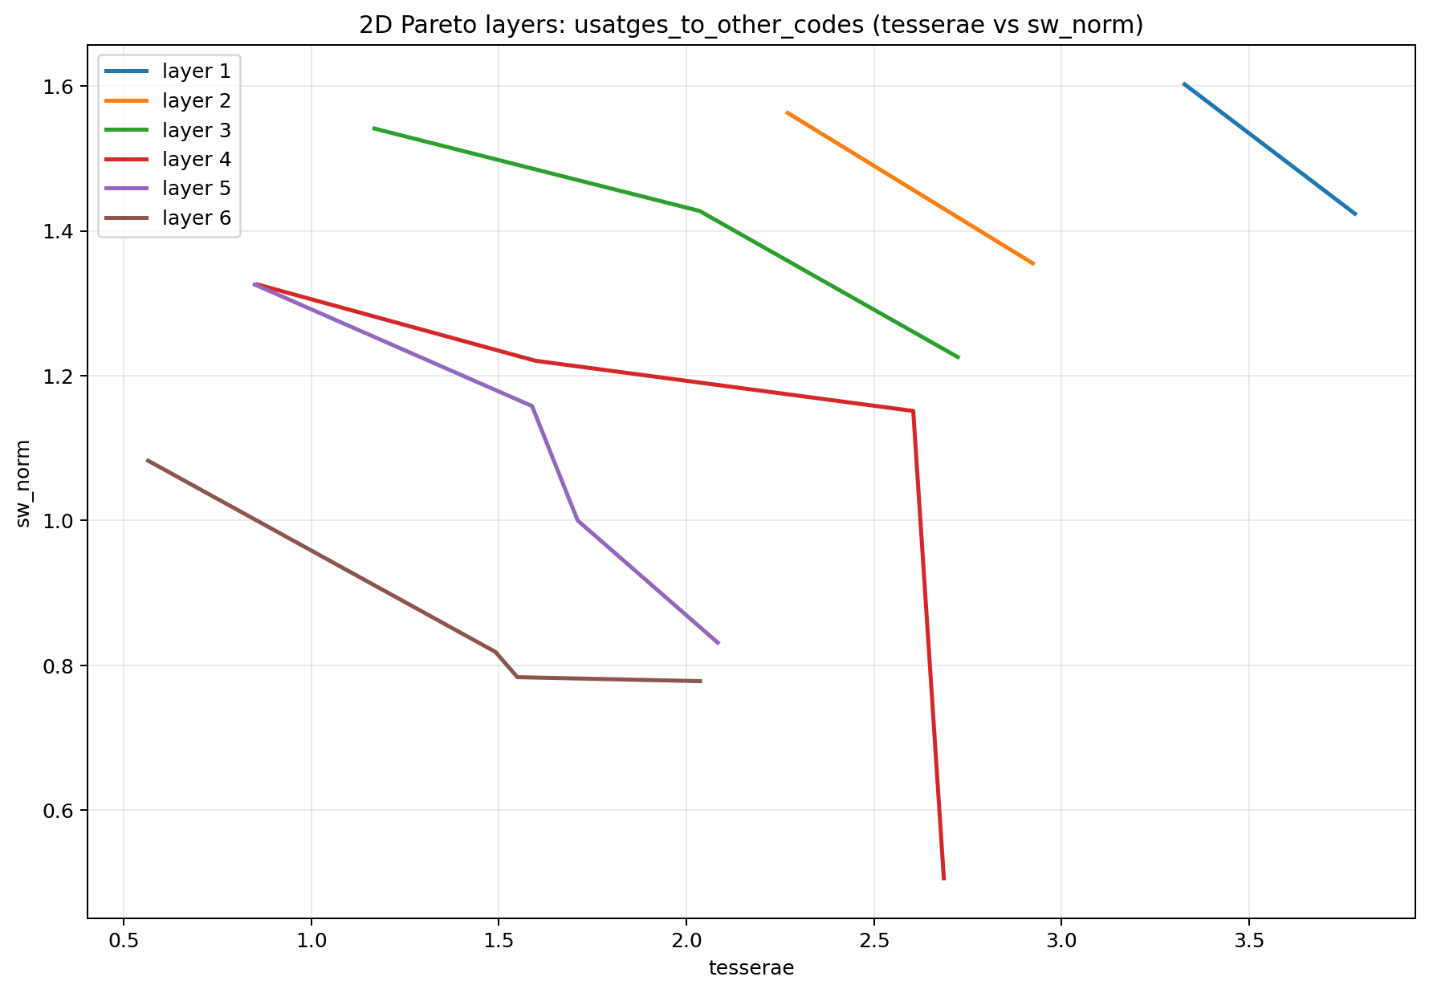
\includegraphics[width=0.95\textwidth]{Dissertation/images/korneeva/chapter1_04.png}
\caption{Двумерные парето-слои для эксперимента между «Барселонскими обычаями» и другими каталонскими сборниками обычного права в пространстве мер Tesserae и $\operatorname{SW}_{\mathrm{norm}}$}
\label{fig:chapter1-04}
\end{figure}

В отличие от предыдущего эксперимента, здесь уже по самой конфигурации слоёв видно, что сильные пары распределены более плотно и компактно в зоне высоких значений обеих метрик. Это закономерно: при сравнении близкородственных нормативных памятников можно ожидать более выраженного пересечения редкой лексики и одновременно более сильного локального выравнивания. Важно подчеркнуть, что такая конфигурация свидетельствует не только о большом числе совпадений, но и о структурной насыщенности самого поля сопоставления. Иными словами, внутри каталонской правовой традиции метод фиксирует устойчивое множество многомерно сильных пар. Именно это объясняет, почему в данном эксперименте используется более глубокая парето-фильтрация: одно лишь сохранение первого слоя было бы слишком жёстким и привело бы к потере значительной части содержательно релевантных соответствий.

\subsection{Нормативные тексты и грамоты}

Третий эксперимент направлен на сопоставление латинских источников и «Барселонских обычаев» с двумя корпусами грамот --- IX--XI~вв. и XII~в. В данной конфигурации граф уже не показывает связи между кодексами и сводами как таковыми, а фиксирует, какие корпуса обнаруживают наибольшее число и наибольшую силу связей с отдельными грамотами.

\begin{figure}[htbp]
\centering
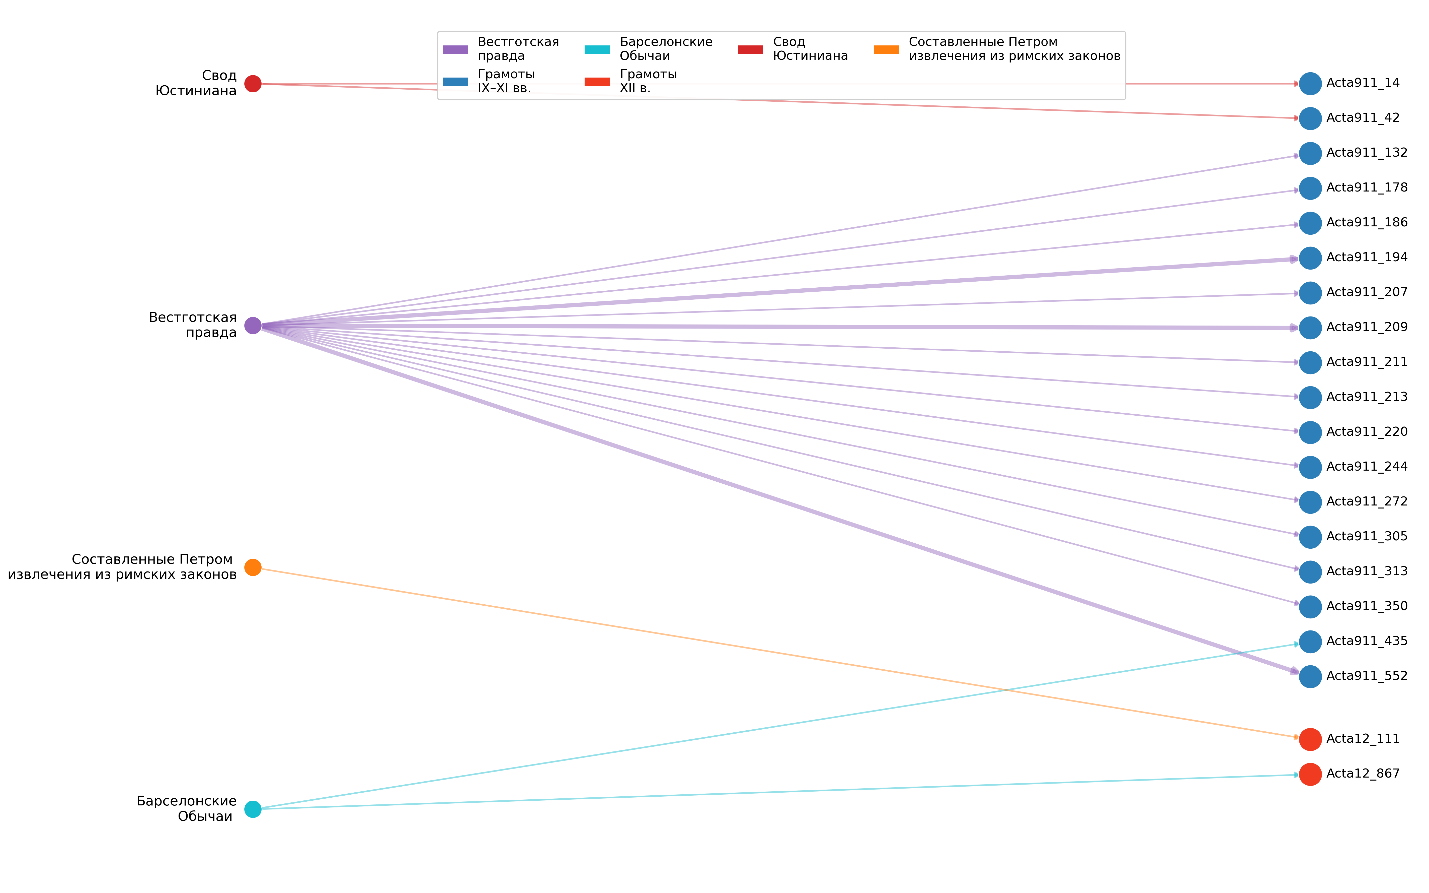
\includegraphics[width=0.95\textwidth]{Dissertation/images/korneeva/chapter1_05.png}
\caption{Граф текстуальных связей между латинскими источниками, «Барселонскими обычаями» и грамотами IX--XII~вв.}
\label{fig:chapter1-05}
\end{figure}

Визуально граф имеет чётко выраженный центр тяжести: подавляющее большинство сильных рёбер исходит от «Вестготской правды», причём эти связи распределяются как по корпусу грамот IX--XI~вв., так и по грамотам XII~в., что позволяет говорить не о случайном совпадении с единичным подкорпусом, а о систематическом присутствии вестготского правового материала в документальном поле. На этом фоне связи с «Барселонскими обычаями», «Сводом гражданского права» Юстиниана, «Вульгатой» и «Составленными Петром извлечениями из римских законов» выглядят существенно более фрагментарными и менее систематическими. Уже сама эта конфигурация представляет серьёзный исследовательский интерес, поскольку она показывает, что в логике данного эксперимента именно «Вестготская правда» выступает главным нормативным ориентиром, с которым соотносятся анализируемые грамоты раннего периода.\emph{ }

\begin{center}
\small
\setlength{\tabcolsep}{2pt}
\begin{longtable}{|p{0.22\textwidth}|p{0.24\textwidth}|p{0.24\textwidth}|p{0.24\textwidth}|}
\caption{Значения метрик и итоговое ранжирование трёх сильнейших соответствий между «Вестготской правдой» и актовым материалом}\label{tab:ch1-charters-ranking}\\
\hline
\textbf{Показатель} & \textbf{\emph{Lex Visigothorum} V.6.3 $\rightarrow$ грамота №~160} & \textbf{\emph{Lex Visigothorum} V.1.1 $\rightarrow$ грамота №~186} & \textbf{\emph{Lex Visigothorum} V.6.3 $\rightarrow$ грамота №~194} \\ \hline
Косинусное сходство & 0,635 (1) & 0,544 (6) & 0,564 (4) \\ \hline
Tesserae & 3,596 (2) & 3,124 (4) & 2,948 (5) \\ \hline
Мягкое косинусное сходство & 0,802 (1) & 0,757 (3) & 0,765 (2) \\ \hline
Нормированное выравнивание & 1,405 (13) & 1,834 (9) & 1,454 (11) \\ \hline
Сумма рангов & 1+2+1+13=\textbf{17} & 6+4+3+9=\textbf{22} & 4+5+2+11=\textbf{22} \\ \hline
Парето-слой & \textbf{1} & \textbf{1} & \textbf{1} \\ \hline
Итоговая позиция & \textbf{1} & \textbf{2} & \textbf{3} \\ \hline
\end{longtable}
\end{center}

Все три пары вошли в первый парето-слой. Первое соответствие получило наименьшую сумму рангов --- 17. Вторая и третья пары имеют одинаковую сумму рангов, однако различаются распределением мест по отдельным показателям. При интерпретации первых двух результатов необходимо учитывать устройство сегментов: высокая позиция отражает сходство с окном, в котором одна и та же глава «Вестготской правды» могла быть процитирована несколько раз применительно к разным актам.

Анализ наиболее сильных совпадений между «Вестготской правдой» и грамотами IX--XI~вв. показывает, что обращение к вестготской правовой традиции в грамотах IX--XI~вв. носило постоянный характер. Наиболее отчётливо это видно в нормах о залоге по долгу и о церковных дарениях: в первом случае в грамотах воспроизводится правило о порядке обращения взыскания на заложенное имущество через судью или иное должностное лицо с последующей оценкой и продажей вещи, во втором --- положение о неотчуждаемости и правовой прочности пожалований, сделанных Церкви. Особенно показательно, что в одном из случаев текст закона вводится в грамоту как прямая цитата со ссылкой на книгу, титул и главу, означающая письменное обоснование конкретного решения. Рассмотрим подробнее эти примеры.

\begin{center}
\small
\setlength{\tabcolsep}{2pt}
\begin{longtable}{|p{\dimexpr0.94\textwidth/3\relax}|p{\dimexpr0.94\textwidth/3\relax}|p{\dimexpr0.94\textwidth/3\relax}|}
\caption{Сопоставление главы V.6.3 «Вестготской правды» и грамоты №~160 о продаже заложенной земли в Сентменате (13 июня 1012~г.)}\label{tab:ch1-charter-160}\\
\hline
\textbf{Элемент сопоставления} & \textbf{«Вестготская правда», V.6.3} & \textbf{Грамота}\textbf{ №~160} \\ \hline
\textbf{Итоговый редуцированный текст} & \emph{reforma}\emph{ }\emph{dissimulet}\emph{ }\emph{diem}\emph{ }\emph{cautionis}\emph{ }\emph{exact}\emph{ }\emph{usque}\emph{ }\emph{decem}\emph{ }\emph{dies}\emph{ }\emph{pignus}\emph{ }\emph{saluum}\emph{ }\emph{domino}\emph{ }\emph{reserue}\emph{ }\emph{eidem}\emph{ }\emph{domino}\emph{ }\emph{propinquo}\emph{ }\emph{reporte}\emph{ }\emph{restituat}\emph{ }\emph{debit}\emph{ }\emph{monea}\emph{ }\emph{neglegenti}\emph{ }\emph{suam}\emph{ }\emph{debitor}\emph{ }\emph{diem}\emph{ }\emph{constitutum}\emph{ }\emph{adesse}\emph{ }\emph{neclexer}\emph{ }\emph{debit}\emph{ }\emph{inple}\emph{ }\emph{distulerit}\emph{ }\emph{addant}\emph{ }\emph{usu}\emph{ }\emph{ceter}\emph{ }\emph{adesse}\emph{ }\emph{usque}\emph{ }\emph{decem}\emph{ }\emph{dies}\emph{ }\emph{sicut}\emph{ }\emph{supra}\emph{ }\emph{scriptum}\emph{ }\emph{deb}\emph{ }\emph{reforma}\emph{ }\emph{dissimulauerit}\emph{ }\emph{tunc}\emph{ }\emph{creditor}\emph{ }\emph{iudici}\emph{ }\emph{preposito}\emph{ }\emph{ciuitatis}\emph{ }\emph{pignus}\emph{ }\emph{ostend}\emph{ }\emph{quant}\emph{ }\emph{iudicio}\emph{ }\emph{trium}\emph{ }\emph{honest}\emph{ }\emph{uirorum}\emph{ }\emph{fuer}\emph{ }\emph{estim}\emph{ }\emph{sit}\emph{ }\emph{licentia}\emph{ }\emph{distrahendi}\emph{ }\emph{postmodum}\emph{ }\emph{pretio}\emph{ }\emph{uenditi}\emph{ }\emph{pigner}\emph{ }\emph{creditor}\emph{ }\emph{quant}\emph{ }\emph{debe}\emph{ }\emph{euident}\emph{ }\emph{toll}\emph{ }\emph{relic}\emph{ }\emph{recipi}\emph{ }\emph{pignus}\emph{ }\emph{seposuer} & \emph{reforma}\emph{ }\emph{dissimulauerit}\emph{ }\emph{tunc}\emph{ }\emph{creditor}\emph{ }\emph{prepositos}\emph{ }\emph{ciuitatis}\emph{ }\emph{pignus}\emph{ }\emph{ostend}\emph{ }\emph{quant}\emph{ }\emph{iudicio}\emph{ }\emph{trium}\emph{ }\emph{onest}\emph{ }\emph{uirorum}\emph{ }\emph{fuer}\emph{ }\emph{extima}\emph{ }\emph{tum}\emph{ }\emph{sid}\emph{ }\emph{licencia}\emph{ }\emph{distraendi}\emph{ }\emph{postmodum}\emph{ }\emph{precio}\emph{ }\emph{uenditi}\emph{ }\emph{pigner}\emph{ }\emph{creditor}\emph{ }\emph{quant}\emph{ }\emph{debeba}\emph{ }\emph{euidenc}\emph{ }\emph{toll}\emph{ }\emph{relic}\emph{ }\emph{recipi}\emph{ }\emph{pignus}\emph{ }\emph{deposuer}\emph{ }\emph{debi}\emph{ }\emph{pignoribus}\emph{ }\emph{transac}\emph{ x }\emph{diebus}\emph{ }\emph{licenti}\emph{ }\emph{habe}\emph{ }\emph{credi}\emph{ }\emph{tor}\emph{ }\emph{uendendi}\emph{ }\emph{donandi}\emph{ }\emph{faciendi}\emph{ }\emph{suam}\emph{ }\emph{uoluntatem}\emph{ }\emph{lu}\emph{ u }\emph{tunc}\emph{ }\emph{creditor}\emph{ }\emph{preposito}\emph{ }\emph{ciuitatis}\emph{ }\emph{pignus}\emph{ }\emph{ostend}\emph{ }\emph{quant}\emph{ }\emph{iudicio}\emph{ }\emph{trium}\emph{ }\emph{honest}\emph{ }\emph{uirorum}\emph{ }\emph{fuer}\emph{ }\emph{extim}\emph{ }\emph{sit}\emph{ }\emph{licencia}\emph{ }\emph{distraendi}\emph{ }\emph{postmodum}\emph{ }\emph{precio}\emph{ }\emph{uenditi}\emph{ }\emph{pigner}\emph{ }\emph{creditor}\emph{ }\emph{quant}\emph{ }\emph{debeb}\emph{ }\emph{euident}\emph{ }\emph{toll}\emph{ }\emph{reliqu}\emph{ }\emph{recipi}\emph{ }\emph{pignus}\emph{ }\emph{deposuer} \\ \hline
\textbf{Текст по изданию} & \emph{Ceterum}\emph{ }\emph{si}\emph{ }\emph{adesse}\emph{ }\emph{usque}\emph{ }\emph{ad}\emph{ }\emph{decem}\emph{ }\emph{dies}\emph{, }\emph{sicut}\emph{ }\emph{supra}\emph{ }\emph{scriptum}\emph{ }\emph{est}\emph{, }\emph{aut}\emph{ }\emph{quod}\emph{ }\emph{debet}\emph{ }\emph{reformare}\emph{ }\emph{dissimulaverit}\emph{, }\emph{tunc}\emph{ }\emph{creditor}\emph{ }\emph{iudici}\emph{ }\emph{vel}\emph{ }\emph{preposito}\emph{ }\emph{civitatis}\emph{ }\emph{pignus}\emph{ }\emph{ostendat}\emph{, }\emph{ut}\emph{, }\emph{quantum}\emph{ }\emph{iudicio}\emph{ }\emph{eius}\emph{ }\emph{et}\emph{ }\emph{trium}\emph{ }\emph{honestorum}\emph{ }\emph{virorum}\emph{ }\emph{fuerit}\emph{ }\emph{estimatum}\emph{, }\emph{sit}\emph{ }\emph{licentia}\emph{ }\emph{distrahendi}\emph{. }\emph{Et postmodum de pretio venditi pigneris creditor, quantum ei debetur, sibi evidentius tollat, et relicum ille recipiat, qui pignus seposuerat}\footnote{LV. V.6.3. P.~345.}\emph{.} & \emph{…reformare dissimulaverit, tunc creditor iudici vel preposito civitatis pignus ostendit, ut quantum iuditio eius vel trium }\emph{honestorum virorum fuerit estimatum, sic licencia ad distrahendi. Et postmodum de precio venditi pingnoris creditor, quantum ei debebatur, sibi evidentius tollat, reliquum illum recipiat qui pingnus deposuerat.}\footnote{Justícia i resolució… 2018. Doc. 160. P.~312--313.}\emph{.} \\ \hline
\textbf{Перевод на русский язык} & … Если же он не явится в течение десяти дней, как сказано выше, или продолжит уклоняться от возвращения долга, кредитор должен представить залог судье или городскому начальнику, чтобы после оценки судьи и трёх добропорядочных мужей получить право продать его. Затем кредитор удерживает из цены проданного залога причитающуюся ему сумму, а остаток получает лицо, передавшее залог. & […] Если должник продолжает уклоняться от возвращения долга, кредитор предъявляет залог судье или городскому начальнику, чтобы после оценки им либо тремя добропорядочными мужами получить право на его продажу. Затем кредитор удерживает из цены проданного залога причитавшуюся ему сумму, а остаток получает лицо, передавшее залог. \\ \hline
\end{longtable}
\end{center}

В грамоте №~160 воспроизведена заключительная часть этой нормы --- предъявление залога должностному лицу, его оценка, продажа, удовлетворение требования кредитора и возвращение остатка собственнику. Совпадение охватывает последовательность действий и специфическую институциональную формулу о судье, городском начальнике и трёх добропорядочных мужах. Поэтому речь идёт о прямом текстовом заимствовании, а не об общем сходстве норм о залоге. Установленный законом десятидневный срок был даже значительно превышен: Бернат утверждал, что после наступления срока исполнения ждал ещё шесть недель. Тем самым составитель грамоты показал, что отчуждение земли произошло после соблюдения предусмотренных письменным законом условий.

Цитата вводится словами \emph{«поэтому по настоянию судьи, как предписывает наш закон»}\footnote{Ibid.:«Idcirco insistente iudice, sicut lex nostra edocet…». P.~312.}. За ней непосредственно следует описание того, как правило было исполнено: продажу совершили в присутствии судьи Борреля, двух его помощников и нескольких названных лиц, которые определили цену земли в четыре манкуса \emph{«}\emph{справедлив}\emph{ой}\emph{»}\footnote{Ibid: «…sicut iustum ab eis preciatum est». P.~313.}.Таким образом, грамота не только воспроизводит положение о судье и добропорядочных мужах, но и документирует участие группы лиц в оценке имущества. Это обстоятельство требует осторожнее интерпретировать замену союза \emph{et} на \emph{vel} в выражении «оценки судьи  (во втором варианте --- либо) трёх добропорядочных мужей»\footnote{Ibid: «…iudicio eius vel trium honestorum virorum…». P.~313.}, т.е. формально текст грамоты допускает оценку судьёй \textbf{либо} тремя добропорядочными мужами. Однако далее указаны и судья Боррель, и сопровождавшие его лица, совместно определившие цену земли. Следовательно, вариант \emph{vel} не привёл в данном случае к изменению процедуры и, вероятнее всего, является свидетельством использования определённой рукописи «Вестготской правды».

Более существенны изменения глагольных форм. В тексте «Вестготской правды» конъюнктив \emph{ostendat} выражает предписание: кредитор должен предъявить залог судье или городскому начальнику. В грамоте использовано изъявительное наклонение того же глагола \emph{ostendit}, благодаря чему содержание нормы сблизилось с рассказом об уже совершённом действии. Форма \emph{debebatur} вместо \emph{debetur} также связывает норму с конкретным обязательством. В исходном тексте речь идёт о сумме, которая причитается кредитору вообще; грамота обозначает задолженность, уже существовавшую к моменту продажи земли. Остальные замены (\emph{seposuerat} на \emph{deposuerat} и формы \emph{pignus}\emph{, }\emph{pigneris} на \emph{pingnus}\emph{, }\emph{pingnoris}) относятся преимущественно к графической адаптации текста и не требуют содержательного анализа. Особого внимания заслуживает совокупность чтений \emph{vel} вместо \emph{et}, \emph{debebatur} вместо \emph{debetur} и \emph{deposuerat} вместо \emph{seposuerat}. Все три варианта совместно представлены в рукописи, обозначенной К.~Цоймером как V¹\footnote{Stockholm, Skoklostersamlingen, 1, E 8641.}. Рукопись относится к XII~в. и потому не могла служить непосредственным источником грамоты 1012~г. Однако совпадение комплекса вариантов позволяет предположить, что цитата в грамоте и текст V¹ восходят к более ранней общей редакции «\emph{Liber}\emph{ }\emph{Iudiciorum}\emph{»}. Среди сохранившихся рукописей именно V¹ представляет ближайшую текстуальную параллель приведённому в грамоте фрагменту.

Итак, составитель сохранил лексику, последовательность процессуальных действий и указание на участвующих в оценке лиц с адаптацией отдельных глагольных форм так, чтобы нормативный текст мог быть включён в изложение уже совершившейся продажи. Высокое место пары в автоматическом ранжировании объясняется протяжённостью совпадающего фрагмента.

Значение этого случая выходит за пределы отдельной грамоты. Та же глава «Вестготской правды» неоднократно привлекалась в каталонских документах. Например, в грамоте №~236 от 8 марта 1032~г., составленной после пятилетней просрочки, продажа заложенного имущества также была совершена в присутствии судьи и четырёх лиц, участвовавших в определении его цены\footnote{Justícia i resolució… 2018. Doc. 236. P.~446--447.}. Это позволяет видеть в грамоте №~160 проявление устойчивой практики цитирования главы V.6.3, а не разовое обращение писца к тексту «Вестготской правды».

Обратимся к анализу следующего по силе соответствия.

\begin{center}
\small
\setlength{\tabcolsep}{2pt}
\begin{longtable}{|p{\dimexpr0.94\textwidth/3\relax}|p{\dimexpr0.94\textwidth/3\relax}|p{\dimexpr0.94\textwidth/3\relax}|}
\caption{Сопоставление главы V.1.1 «Вестготской правды» и грамоты №~186 о возвращении монастырю Санта-Мария-де-Серратейш аллодов Пужол и Вивер (Берга, 27 января 1020~г.)}\label{tab:ch1-charter-186}\\
\hline
\textbf{Элемент сопоставления} & \textbf{«Вестготская правда», V.1.1} & \textbf{Грамота}\textbf{ №~186} \\ \hline
\textbf{Итоговый редуцированный текст} & \emph{quapropter}\emph{ }\emph{quecum}\emph{ }\emph{res}\emph{ }\emph{sanc}\emph{ }\emph{dei}\emph{ }\emph{basilicis}\emph{ }\emph{principum}\emph{ }\emph{quoramlib}\emph{ }\emph{fidel}\emph{ }\emph{donation}\emph{ }\emph{conlate}\emph{ }\emph{repperiun}\emph{ }\emph{uoti}\emph{ }\emph{potentialiter}\emph{ }\emph{certo}\emph{ }\emph{cense}\emph{ }\emph{earum}\emph{ }\emph{iure}\emph{ }\emph{inreuocabili}\emph{ }\emph{modo}\emph{ }\emph{legum}\emph{ }\emph{eternitate}\emph{ }\emph{firment} & \emph{precip}\emph{ }\emph{libr}\emph{ }\emph{iudic}\emph{ }\emph{libr}\emph{ }\emph{quint}\emph{ }\emph{donation}\emph{ }\emph{ecclesi}\emph{ }\emph{fac}\emph{ }\emph{dicens}\emph{ }\emph{quapropter}\emph{ }\emph{quasc}\emph{ }\emph{res}\emph{ }\emph{sunt}\emph{ }\emph{dei}\emph{ }\emph{basilicis}\emph{ }\emph{principium}\emph{ }\emph{quarumlibet}\emph{ }\emph{fidel}\emph{ }\emph{donation}\emph{ }\emph{collate}\emph{ }\emph{reperiun}\emph{ }\emph{uoti}\emph{ }\emph{potencialiter}\emph{ }\emph{certo}\emph{ }\emph{cense}\emph{ }\emph{earum}\emph{ }\emph{iure}\emph{ }\emph{inreuocabili}\emph{ }\emph{modo}\emph{ }\emph{legum}\emph{ }\emph{aternitate}\emph{ }\emph{firment} \\ \hline
\textbf{Текст по изданию} & \emph{Quapropter}\emph{, }\emph{quecumque}\emph{ }\emph{res}\emph{ }\emph{sanctis}\emph{ Dei }\emph{basilicis}\emph{ }\emph{aut}\emph{ }\emph{per}\emph{ }\emph{principum}\emph{ }\emph{aut}\emph{ }\emph{per}\emph{ }\emph{quoramlibet}\emph{ }\emph{fidelium}\emph{ }\emph{donationes}\emph{ }\emph{conlate}\emph{ }\emph{repperiuntur}\emph{ }\emph{votive}\emph{ }\emph{ac}\emph{ }\emph{potentialiter}\emph{, }\emph{pro}\emph{ }\emph{certo}\emph{ }\emph{censetur} (возможен вариант --- \emph{censemus})\emph{, ut in }\emph{earum}\emph{ }\emph{iure}\emph{ }\emph{inrevocabili}\emph{ }\emph{modo}\emph{ }\emph{legum}\emph{ }\emph{eternitate}\emph{ }\emph{firmentur}\footnote{LV. V.1.1. P.~207.}\emph{.} & \emph{Ubi}\emph{ }\emph{precipit}\emph{ in }\emph{Libro}\emph{ }\emph{Iudicum}\emph{, in }\emph{libro}\emph{ }\emph{quinto}\emph{ de }\emph{donationibus}\emph{ }\emph{Ecclesie}\emph{ }\emph{factis}\emph{, }\emph{dicens}\emph{: «}\emph{Quapropter}\emph{ }\emph{quascumque}\emph{ }\emph{res}\emph{ }\emph{si}\emph{ }\emph{sunt}\emph{ Dei }\emph{basilicis}\emph{ }\emph{aut}\emph{ }\emph{principium}\emph{ }\emph{aut}\emph{ }\emph{quarumlibet}\emph{ }\emph{fidelium}\emph{ }\emph{donationes}\emph{ }\emph{collate}\emph{ }\emph{reperiuntur}\emph{ }\emph{votive}\emph{ }\emph{ac}\emph{ }\emph{potencialiter}\emph{ }\emph{pro}\emph{ }\emph{certo}\emph{ }\emph{censemus}\emph{ ut in }\emph{earum}\emph{ }\emph{iure}\emph{ }\emph{inrevocabili}\emph{ }\emph{modo}\emph{ }\emph{legum}\emph{ }\emph{aternitate}\emph{ }\emph{firmentur}\emph{»}\emph{\textsuperscript{ }}\footnote{Justícia i resolució... 2018. Doc. 186. P.~362--363.}\emph{.} \\ \hline
\textbf{Перевод на русский язык} & Поэтому всякое имущество, которое оказывается переданным святым Божьим базиликам посредством дарений правителей или любых верующих по обету и на законном основании несомненно должно быть навечно утверждено за ними незыблемой силой закона. & Поэтому всякое имущество, которое оказывается переданным святым Божьим базиликам посредством дарений правителей или любых верующих по обету и на законном основании мы постановляем навечно утвердить за ними незыблемой силой закона. \\ \hline
\end{longtable}
\end{center}

Грамота №~186 о возвращении монастырю Санта-Мария-де-Серратейш аллодов Пужол и Вивер воспроизводит главу V.1.1 «Вестготской правды» почти полностью. Протяжённость текста и сохранение его риторического построения исключают независимое возникновение формулы.

Большинство различий сводится к орфографии: \emph{collate}\emph{ }меняется на\emph{ }\emph{conlate}\emph{, }\emph{reperiuntur}\emph{ }--- на \emph{repperiuntur}\emph{, }\emph{potencialiter}\emph{ }--- на \emph{potentialiter}\emph{, }\emph{aternitate}\emph{ }--- на\emph{ }\emph{eternitate}\emph{.} Существеннее изменение \emph{censetur} на \emph{censemus}. В «Вестготской правде» заключение выражено безлично (\emph{censetur}): \emph{«}\emph{установленным считается, что церковные дарения должны быть утверждены навечно}\emph{»}\footnote{LV. V.1.1: «…pro certo censetur, ut in earum iure inrevocabili modo legum eternitate firmentur~…». P.~207. В критическом аппарате к этому месту отмечено чтение \emph{censemus} в части рукописей.}. В тексте грамоты появляется первое лицо множественного числа: \emph{«мы постановляем»} (\emph{cense}\emph{mus})\footnote{Justícia i resolució... 2018. Doc. 186: «…pro certo censemus ut in earum iure inrevocabili modo legum aternitate firmentur…». P.~363.}. При этом использование первого лица множественного числа в активном залоге не обязательно следует интерпретировать как сознательную замену безличного оборота на «мы постановляем», произведённую составителем грамоты. Такое чтение могло уже находиться в использованном списке «Вестготской правды». Это подтверждается и каталонским материалом: \emph{censemus} встречается в цитатах V.1.1 в грамотах №~186, 207, 292 и 391, тогда как грамота №~244 сохраняет чтение \emph{censetur}\footnote{Justícia i resolució... 2018. P.~1061--1062.}.

Цитата сохраняет самостоятельность внутри документа. После неё следует собственно судебное распоряжение: \emph{«И на основании этого установления мы возвращаем его во власть Святой Марии»}\footnote{Justícia i resolució... 2018. Doc. 186.: «… Et pro hac ordinatione reddimus eum in potestatem Sancte Marie ». P.~363.}. Таким образом, норма V.1.1 выступает здесь как прямо обозначенный текст закона, которым судья обосновывает возвращение имущества монастырю.

Обратимся к следующему примеру.

\begin{center}
\small
\setlength{\tabcolsep}{2pt}
\begin{longtable}{|p{\dimexpr0.94\textwidth/3\relax}|p{\dimexpr0.94\textwidth/3\relax}|p{\dimexpr0.94\textwidth/3\relax}|}
\caption{Сопоставление главы V.6.3 «Вестготской правды» и записи судебного заседания по жалобе аббата Санта-Мария-де-Жерри на Алегрета де Клавероля и его братьев (18 февраля 1138~г., замок Салас-де-Пальярс; грамота №~194)}\label{tab:volume1-last}\\
\hline
\textbf{Элемент сопоставления} & \textbf{«Вестготская правда», V.6.3} & \textbf{Грамота}\textbf{ №~194} \\ \hline
\textbf{Итоговый редуцированный текст} & \emph{pigne}\emph{ }\emph{debito}\emph{ }\emph{depona}\emph{ }\emph{pignus}\emph{ }\emph{debito}\emph{ }\emph{deponi}\emph{ }\emph{cautionem}\emph{ }\emph{fuer}\emph{ }\emph{obligatum}\emph{ }\emph{pignus}\emph{ }\emph{deposuer}\emph{ }\emph{tempus}\emph{ }\emph{constitutum}\emph{ }\emph{debit}\emph{ }\emph{reforma}\emph{ }\emph{dissimulet}\emph{ }\emph{diem}\emph{ }\emph{cautionis}\emph{ }\emph{exact}\emph{ }\emph{usque}\emph{ }\emph{decem}\emph{ }\emph{dies}\emph{ }\emph{pignus}\emph{ }\emph{saluum}\emph{ }\emph{domino}\emph{ }\emph{reserue}\emph{ }\emph{eidem}\emph{ }\emph{domino}\emph{ }\emph{propinquo}\emph{ }\emph{reporte}\emph{ }\emph{restituat}\emph{ }\emph{debit}\emph{ }\emph{monea}\emph{ }\emph{neglegenti}\emph{ }\emph{suam}\emph{ }\emph{debitor}\emph{ }\emph{diem}\emph{ }\emph{constitutum}\emph{ }\emph{adesse}\emph{ }\emph{neclexer}\emph{ }\emph{debit}\emph{ }\emph{inple}\emph{ }\emph{distulerit}\emph{ }\emph{addant}\emph{ }\emph{usu}\emph{ }\emph{ceter}\emph{ }\emph{adesse}\emph{ }\emph{usque}\emph{ }\emph{decem}\emph{ }\emph{dies}\emph{ }\emph{sicut}\emph{ }\emph{supra}\emph{ }\emph{scriptum}\emph{ }\emph{deb}\emph{ }\emph{reforma}\emph{ }\emph{dissimulauerit}\emph{ }\emph{tunc}\emph{ }\emph{creditor}\emph{ }\emph{iudici}\emph{ }\emph{preposito}\emph{ }\emph{ciuitatis}\emph{ }\emph{pignus}\emph{ }\emph{ostend}\emph{ }\emph{quant}\emph{ }\emph{iudicio}\emph{ }\emph{trium}\emph{ }\emph{honest}\emph{ }\emph{uirorum}\emph{ }\emph{fuer}\emph{ }\emph{estim}\emph{ }\emph{sit}\emph{ }\emph{licentia}\emph{ }\emph{distrahendi}\emph{ }\emph{postmodum}\emph{ }\emph{pretio}\emph{ }\emph{uenditi}\emph{ }\emph{pigner}\emph{ }\emph{creditor}\emph{ }\emph{quant}\emph{ }\emph{debe}\emph{ }\emph{euident}\emph{ }\emph{toll}\emph{ }\emph{relic}\emph{ }\emph{recipi}\emph{ }\emph{pignus}\emph{ }\emph{seposuer} & \emph{quem}\emph{ }\emph{lex}\emph{ }\emph{continetur}\emph{ u }\emph{titulo}\emph{ }\emph{ui}\emph{ }\emph{capitula}\emph{ }\emph{iii}\emph{ }\emph{dic}\emph{ }\emph{pignus}\emph{ }\emph{debito}\emph{ }\emph{deponi}\emph{ }\emph{debito}\emph{ }\emph{deponi}\emph{ }\emph{cautionem}\emph{ }\emph{fuer}\emph{ }\emph{obligatum}\emph{ }\emph{pignus}\emph{ }\emph{deposuer}\emph{ }\emph{tempus}\emph{ }\emph{constitutum}\emph{ }\emph{debit}\emph{ }\emph{reforma}\emph{ }\emph{dissimulet}\emph{ }\emph{diem}\emph{ }\emph{cautionis}\emph{ }\emph{exact}\emph{ }\emph{usque}\emph{ }\emph{decem}\emph{ }\emph{dies}\emph{ }\emph{pignus}\emph{ }\emph{saluum}\emph{ }\emph{domino}\emph{ }\emph{reserue}\emph{ }\emph{eidem}\emph{ }\emph{domino}\emph{ }\emph{propinquo}\emph{ }\emph{reporte}\emph{ }\emph{restituat}\emph{ }\emph{debit}\emph{ }\emph{monea}\emph{ }\emph{neglegenti}\emph{ }\emph{suam}\emph{ }\emph{debitor}\emph{ }\emph{debit}\emph{ }\emph{imple}\emph{ }\emph{distulerit}\emph{ }\emph{addant}\emph{ }\emph{usu}\emph{ }\emph{certe}\emph{ }\emph{debit}\emph{ }\emph{reforma}\emph{ }\emph{dissimulauerit}\emph{ }\emph{tunc}\emph{ }\emph{creditor}\emph{ }\emph{preposito}\emph{ }\emph{ciuitatis}\emph{ }\emph{pignus}\emph{ }\emph{ostend}\emph{ }\emph{quant}\emph{ }\emph{iudicio}\emph{ }\emph{trium}\emph{ }\emph{honest}\emph{ }\emph{uirorum}\emph{ }\emph{fuer}\emph{ }\emph{estim}\emph{ }\emph{sit}\emph{ }\emph{licen}\emph{ }\emph{tia}\emph{ }\emph{distrahendi}\emph{ }\emph{postmodum}\emph{ }\emph{precio}\emph{ }\emph{uenditi}\emph{ }\emph{pigner}\emph{ }\emph{creditor}\emph{ }\emph{quant}\emph{ }\emph{debe}\emph{ }\emph{euident}\emph{ }\emph{toll}\emph{ }\emph{reliq}\emph{ }\emph{recipi}\emph{ }\emph{pignus}\emph{ }\emph{deposuer}\emph{ }\emph{comodis}\emph{ }\emph{iudicum}\emph{ }\emph{saion}\emph{ }\emph{lex}\emph{ }\emph{continetur}\emph{ }\emph{titulo} \\ \hline
\textbf{Текст по изданию} & \emph{De pignere, si pro debito deponatur. Pignus, quod pro debito deponitur, si per cautionem fuerit obligatum, et ille, qui pignus deposuerat, ad tempus constitutum debitum reformare dissimulet, post diem cautionis exactum usque ad decem dies pignus salvum suo domino reservetur aut eidem domino, si in propinquo est, reportetur, atque, ut restituat debitum, moneatur. Quod si per neglegentiam suam debitor ad diem constitutum adesse neclexerit aut debitum inplere distulerit, addantur }\emph{usure. Ceterum si adesse usque ad decem dies, sicut supra scriptum est, aut quod debet reformare dissimulaverit, tunc creditor iudici vel preposito civitatis pignus ostendat, ut, quantum iudicio eius et trium honestorum virorum fuerit estimatum, sit licentia distrahendi. }\emph{Et postmodum de pretio venditi pigneris creditor, quantum ei debetur, sibi evidentius tollat, et relicum ille recipiat, qui pignus seposuerat}\footnote{LV. V.6.3. P.~232.}\emph{.} & \emph{Quem lex que continetur libro V, titulo VI, capitula III, ita dicit: «Pignus quod pro debito deponitur, si pro debito deponitur, si per cautionem fuerit obligatum et ille qui pignus deposuerat ad tempus constitutum debitum reformare dissimulet, post diem cautionis exactum usque ad decem dies pignus salvum domino reservetur aut eidem domino, si in propinquo est, reportetur atque ut restituat debitum moneatur. }\emph{Quod}\emph{ }\emph{si}\emph{ per }\emph{neglegentiam}\emph{ }\emph{suam}\emph{ }\emph{debitor}\emph{ }\emph{debitum}\emph{ }\emph{implere}\emph{ }\emph{distulerit}\emph{, }\emph{addantur}\emph{ usure. }\emph{Certe}\emph{ }\emph{si}\emph{ }\emph{debitum}\emph{ }\emph{reformare}\emph{ }\emph{dissimulaverit}\emph{, tunc }\emph{creditor }\emph{iudici}\emph{ vel }\emph{preposito}\emph{ civitatis pignus }\emph{ostendat}\emph{, ut quantum }\emph{iudicio}\emph{ eius vel }\emph{trium}\emph{ }\emph{honestorum}\emph{ }\emph{virorum}\emph{ }\emph{fuerit}\emph{ }\emph{estimatum}\emph{, sit }\emph{licentia}\emph{ }\emph{distrahendi}\emph{. }\emph{Et postmodum de precio venditi pigneris creditor, quantum ei debetur, sibi evidentius tollat et reliqum ille recipiat qui pignus deposuerat»}\footnote{Justícia i resolució... 2018. Doc. 194. P.~375--376.}\emph{.} \\ \hline
\textbf{Перевод на русский язык} & \textbf{О залоге, переданном в обеспечение долга.} Залог, переданный в обеспечение долга, если он был обусловлен письменным обязательством и тот, кто его передал, уклоняется от возвращения долга к установленному сроку, после истечения срока обязательства должен в течение десяти дней сохраняться для своего владельца либо, если владелец находится поблизости, быть доставлен ему; при этом владельца следует уведомить о необходимости возвратить долг. Если должник по небрежности не явится в установленный день или отсрочит уплату долга, начисляются проценты. Если же он не явится в течение десяти дней, как сказано выше, или продолжит уклоняться от возвращения долга, кредитор должен представить залог судье или городскому начальнику, чтобы после оценки судьи и трёх добропорядочных мужей получить право продать его. Затем кредитор удерживает из цены проданного залога причитающуюся ему сумму, а остаток получает лицо, передавшее залог. & Оставшуюся часть золота я удерживаю у себя, чтобы упомянутый выше иудей за вычетом вознаграждения названных судей получил её как лицо, передавшее залог. Закон, содержащийся в книге V, титуле VI, главе III, гласит: «Залог, переданный в обеспечение долга, если он был обусловлен письменным обязательством и тот, кто его передал, уклоняется от возвращения долга к установленному сроку, после истечения срока обязательства должен в течение десяти дней сохраняться для своего владельца либо, если владелец находится поблизости, быть доставлен ему; при этом владельца следует уведомить о необходимости возвратить долг. Если должник по своей небрежности откладывает уплату долга, начисляются проценты. Если он продолжает уклоняться от возвращения долга, кредитор должен представить залог судье или городскому начальнику, чтобы после оценки им либо тремя добропорядочными мужами получить право продать его. Затем кредитор удерживает из цены проданного залога причитающуюся ему сумму, а остаток получает лицо, передавшее залог». \\ \hline
\end{longtable}
\end{center}

Грамота №~194 представляет наиболее надёжный пример из трёх, поскольку прямая цитата из «Вестготской правды» в данном случае снабжена точной ссылкой: книга V, титул VI, глава III. Основное содержание нормы заключалось в следующем: после продажи заложенного имущества кредитор должен был удержать причитающуюся ему сумму, а остаток за вычетом вознаграждения судей следовало передать лицу, предоставившему залог. Ссылка на «Вестготскую правду» непосредственно обосновывает порядок распределения полученной цены.

Цитата несколько сокращает исходную статью. Из неё устранено повторное указание на неявку должника в течение десяти дней, а переход\footnote{LV. V.6.3: «Ceterum si adesse usque ad decem dies…». P.~232.} заменён краткой формулой\footnote{Justícia i resolució... 2018. Doc. 194: «Certe si debitum reformare dissimulaverit...». P.~376.}. Тем самым сохранилась последовательность основных действий, но были устранены детали, не имевшие непосредственного значения для описываемого случая. В отличие от грамоты №~160, здесь можно наблюдать практически полный текст нормы, адаптированный к фактическим обстоятельствам сделки.

Особенно важно совпадение вариантов в грамотах №~160 и 194\footnote{См. выше.}. Совокупность одинаковых чтений позволяет предположить, что составители двух актов обращались к одной и той же рукописи V\textsuperscript{1} или к одной циркулировавшей в каталонской актовой практике редакции главы V.6.3 в близких списках общего происхождения.

В совокупности три соответствия показывают разные способы адаптации норм «Вестготской правды» в актовом материале:

\begin{itemize}
\item в грамоте №~160 из главы извлечена только часть, регулирующая продажу залога;
\item в грамоте №~186 почти вся норма о церковных дарениях включена в структуру документа с общей ссылкой на «Вестготскую правду» и адаптирована к содержанию документа;
\item в грамоте №~194 глава V.6.3 процитирована с прямой ссылкой и использована для разрешения конкретного имущественного спора.
\end{itemize}
Повторное использование одной и той же нормы о залоге с общими текстологическими вариантами свидетельствует не только об авторитетности «\emph{Liber}\emph{ }\emph{Iudiciorum}», но и о существовании устойчивой рукописной традиции, посредством которой нормы «Вестготской правды» были включены в каталонскую правовую культуру указанного периода.

То обстоятельство, что выделенные пары соответствуют тем, которые были определены классическими текстологическими методиками\footnote{Justícia i resolució… 2024. P.~1061--1063.}, дополнительно подтверждает возможность применения разработанного нами алгоритма для актового материала. Парето-схема в данном случае также оказывается показательна.

\begin{figure}[htbp]
\centering
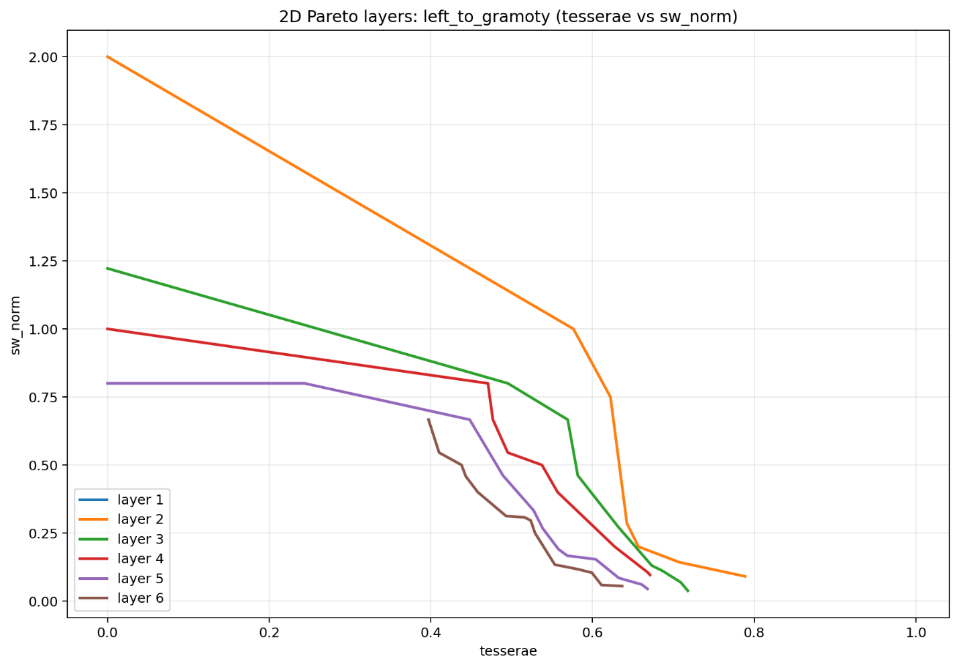
\includegraphics[width=0.95\textwidth]{Dissertation/images/korneeva/chapter1_06.png}
\caption{Двумерные парето-слои для эксперимента сравнения между латинскими источниками, «Барселонскими обычаями» и грамотами IX--XII~вв. в пространстве мер Tesserae и $\operatorname{SW}_{\mathrm{norm}}$}
\label{fig:chapter1-06}
\end{figure}

Здесь видно, что слои расположены сравнительно близко к низким значениям обеих метрик, а первый слой с сильными парами практически вырожден. Пространство сильных пар в данном эксперименте в целом менее насыщено, чем в случае прямого сопоставления нормативных памятников. Такая картина соответствует природе актового материала: в текстах грамот редко воспроизводят нормативные формулы столь же плотно и регулярно, как это происходит при сопоставлении сводов обычного права. Следовательно, даже при наличии «сильных» рёбер в графе большая часть результатов располагается в зоне умеренных значений. Методологически это важно, поскольку показывает: эксперимент с грамотами должен интерпретироваться как выявление отдельных правовых формул, частичных заимствований и следов общего правового языка.

\section{Возможности и ограничения метода, сравнение возможностей с классическими методами}

\subsection{Исследовательские ограничения метода}

Несмотря на аналитические возможности предложенного подхода, его применение сопряжено с рядом ограничений, которые необходимо учитывать при интерпретации результатов. Прежде всего метод выявляет текстуальную близость, но сам по себе не позволяет автоматически отождествлять её с прямым заимствованием, генетической зависимостью или однозначно установленным влиянием одного памятника на другой. Совпадение может быть обусловлено различными причинами --- общностью правовой традиции, использованием сходных формул, обращением к промежуточному источнику, жанровой конвенцией или (в отдельных случаях) случайным пересечением лексики. Следовательно, вычислительно обнаруженная связь должна рассматриваться не как окончательное доказательство, а как аналитически значимый индикатор, требующий последующей историко-филологической верификации.

Существенным ограничением метода является зависимость его результатов от качества исходного текста. Публикации исторических источников содержат следы редакторского вмешательства, вариативную орфографию, смешение языковых слоёв, а также ошибки, возникающие в процессе оптического распознавания текста. Даже при наличии специально разработанных процедур очистки, нормализации и редукции словоформ полностью устранить влияние подобных факторов невозможно. Вследствие этого часть сильных пар может оказаться методически подозрительной, если она формируется на базе дефектного сегмента или искажённого чтения. Особенно наглядно это проявляется в экспериментах с актовым материалом, где отдельные рёбра графа требуют дополнительной проверки уже на уровне источника.

Ограничения связаны и с самой природой формализуемых текстуальных признаков. Метод строится на сочетании нескольких метрик, каждая из которых фиксирует определённый аспект сходства --- общую лексическую близость, пересечение по редкой лексике, частичное формальное совпадение словоформ и локальное выравнивание последовательностей. Ни одна из этих мер не исчерпывает всего многообразия форм текстуального родства. В частности, алгоритм с трудом улавливает случаи глубокой смысловой переработки, когда смысловое ядро нормы сохраняется при значительной лексической перестройке.

Отдельное ограничение связано с выбором масштаба анализа. Хотя введение структурного сегментирования и регулируемого дробления на окна позволяет согласовать вычислительный уровень с природой источника, этот баланс не может считаться достигнутым раз и навсегда. Слишком крупный сегмент способен скрывать локальное совпадение, тогда как чрезмерно мелкое дробление приводит к утрате смысловой целостности. Поэтому параметры окна, перекрытия и минимальной длины сегмента неизбежно сохраняют характер исследовательского компромисса. Это означает, что результаты чувствительны к настройкам выбранной конфигурации, сами эти настройки задаются не произвольно, а с опорой на распределение длин сегментов в корпусе.

Необходимо учитывать и ограничения, связанные с предварительным отбором кандидатов. Используемый на четвёртом этапе вычислительный бюджет делает задачу практически осуществимой, однако одновременно вводит контролируемое сокращение пространства сравнений. На последующие стадии анализа попадает наиболее перспективная часть пар внутри их изначального множества. Таким образом, метод гарантирует не исчерпывающий перебор всех теоретически возможных параллелей, а воспроизводимую и вычислительно обоснованную работу с ограниченным множеством наиболее правдоподобных кандидатов.

Сходным образом ограничения касаются и этапа многослойной фильтрации. Парето-подход позволяет избежать произвольного сведения всех метрик к одной шкале и сохраняет разные типы сильных профилей сходства, однако и он не устраняет полностью проблему исследовательского выбора. Решение о числе сохраняемых парето-слоёв влияет на то, насколько строгим или, напротив, расширительным окажется итоговый отбор. Если сохраняется лишь первый слой, исследование получает максимально строгий, но сравнительно узкий набор соответствий. Если слоёв сохраняется больше, возрастает полнота результата, но одновременно усложняется его интерпретация. Таким образом, даже при высокой степени формализации метод не устраняет необходимости в исследовательском суждении, а лишь переводит его в более прозрачную и контролируемую форму.

Наконец, ограничение касается самого статуса итоговых графов и сводных карт. Графическая репрезентация позволяет выявлять центральные и периферийные узлы, плотные кластеры и основные линии текстуального взаимодействия, однако она неизбежно связана с процедурой агрегирования и отбора. Визуализированный граф не воспроизводит всей полноты исходного массива соответствий, а представляет собой его аналитически сокращённую и упорядоченную проекцию. Поэтому графические материалы следует рассматривать не как непосредственное «изображение традиции», а как инструмент её структурного моделирования. Их задача состоит не в том, чтобы заменить анализ конкретных совпадений, а в том, чтобы сделать обозримой общую конфигурацию связей, подлежащую дальнейшему содержательному осмыслению.

Таким образом, ограничения метода не отменяют его исследовательской ценности, но задают рамки корректной интерпретации результатов. Предлагаемый подход позволяет систематически выявлять, структурировать и визуализировать текстуальные связи в сложных исторических корпусах, однако его выводы приобретают полноценную доказательную силу лишь в сочетании с качественным источниковедческим, текстологическим и историко-правовым анализом. Именно в таком сочетании вычислительная процедура выступает не как самодостаточная альтернатива традиционным методам, а как их продуктивное дополнение, расширяющее возможности работы с корпусом и повышающее степень аналитической обозримости материала.

\subsection{Преимущества применяемого метода}

К числу основных достоинств предлагаемого метода относится прежде всего его многоуровневый характер. В отличие от подходов, в которых анализ текстуального родства сводится к одной универсальной мере или к единственному масштабу сопоставления, рассматриваемая процедура последовательно учитывает структурную организацию источника, различия в размере сегментов, неоднородность языкового материала, множественность форм текстуальной близости. Благодаря этому метод позволяет переходить от локального совпадения отдельного пассажа к более общим конфигурациям связей между статьями, памятниками и корпусами в целом, не утрачивая при этом связи между этими уровнями анализа.

Не менее важным преимуществом является адаптивность метода по отношению к природе исторического материала. Источники, включённые в исследование, различаются по языку, жанру, внутренней структуре, степени сохранности и характеру редакционного оформления. Метод учитывает эти различия уже на ранних стадиях обработки: сегментирование осуществляется с опорой на собственную структурную единицу источника, дробление на окна применяется выборочно, а предварительная обработка зависит от режима сегмента и его языковых характеристик. Подобная настройка делает возможной работу с гетерогенным корпусом без искусственного сведения всех источников к одному и тому же формальному шаблону. В результате вычислительная процедура оказывается согласованной с историко-текстуальной спецификой материала.

Существенным достоинством метода является и то, что он не подменяет сложное явление текстуального родства одной шкалой сходства. Использование нескольких метрик --- общей лексической близости, пересечения по редкой лексике, мягкого совпадения вариативных форм и локального выравнивания --- позволяет учитывать разные типы соответствий, которые могут иметь различную историческую природу. Это особенно важно для правовых текстов, где связь между двумя фрагментами может выражаться либо в буквальном воспроизведении формулы, либо в устойчивом наборе редких терминов, либо в переработанном, но явно узнаваемом обороте.

Отдельного внимания заслуживает прозрачность процедуры отбора результатов. Благодаря использованию предварительного отбора по TF-IDF и последующей многослойной парето-фильтрации исследователь получает возможность не только очертить будущее пространство сравнений, но и сделать логику этого сокращения методически обозримой. При использовании данного метода мы старались избежать произвольного сведения множества показателей к одному итоговому числу и избыточного числа мер близости текстов. В рамках метода сохраняются разные типы сильных соответствий. Их ранжирование и визуализация в виде графов прозрачно управляются исследователем.

Ещё одно существенное преимущество связано с воспроизводимостью и документированностью всей процедуры. Параметры экспериментов задаются в отдельном конфигурационном файле, а результаты фиксируются не только в виде таблиц и графов, но и в форме markdown-отчётов, содержащих перечни сильнейших соответствий, значения метрик и примеры текстовых фрагментов. Это означает, что исследователь может не только повторить эксперимент в идентичной конфигурации, но и проследить переход от общей структуры графа к конкретным сегментам, лежащим в основе отдельных рёбер. Подобная организация особенно ценна для историко-квантитативного исследования, поскольку она соединяет вычислительную строгость с возможностью содержательной проверки и интерпретации каждого значимого результата.

Наконец, важнейшим достоинством метода является его интерпретируемость в гуманитарном смысле. Итогом анализа становится не только массив числовых оценок или набор трудно обозримых совпадений, но и система графов и сводных карт, в которой становятся различимыми центральные и периферийные узлы, плотные кластеры и основные направления текстуального взаимодействия. Такая форма представления результатов позволяет переводить вычислительно найденные связи в пространство историко-филологического обсуждения. Метод, таким образом, не замыкается на уровне алгоритмической обработки, а создаёт условия для перехода к содержательным выводам о структуре правовой традиции, о распределении заимствований и о месте отдельных памятников в системе текстуальных взаимоотношений.

В совокупности перечисленные особенности позволяют рассматривать предлагаемый подход как продуктивный инструмент исследования сложных исторических текстов. Его преимущество состоит не только в способности выявлять отдельные текстуальные совпадения, но и в возможности связывать эти совпадения с более широкими вопросами историко-правовой и текстологической интерпретации. Именно в этом сочетании формализованной процедуры, адаптивности, воспроизводимости и интерпретируемости и заключается основная исследовательская ценность метода.

\section*{Выводы к Главе 1}
\addcontentsline{toc}{section}{Выводы к Главе 1}

Проведённый в данной главе анализ позволяет сделать вывод о том, что вычислительный подход, основанный на многоэтапном сопоставлении сегментов, расчёте нескольких метрик близости, парето-фильтрации и графовой репрезентации результатов, оказывается продуктивным не только как методическая процедура, но и как средство получения содержательно значимых историко-правовых наблюдений. Его применение к корпусам латинских источников, каталонских сборников обычного права и грамот показывает, что текстуальные связи внутри исследуемого материала распределены неравномерно, но в то же время обнаруживают устойчивую и интерпретируемую структуру.

Сопоставление «Барселонских обычаев» с другими каталонскими сборниками обычного права позволяет заключить, что внутри самой каталонской традиции текстуальное родство носит выраженно структурированный характер. Наиболее тесные связи обнаруживаются с «Обычаями Тортосы», что проявляется как в общей конфигурации графа, так и в конкретных топ-парах, где совпадения затрагивают порядок изложения нормы, набор юридически значимых действий и систему санкций. Следовательно, «Барселонские обычаи» следует помещать в пространство не абстрактной региональной общности, а в более конкретную сеть тесно взаимодействующих нормативных памятников, внутри которой одни сборники оказываются значительно ближе друг к другу, чем другие. В этом отношении вычислительный анализ не только подтверждает качественные наблюдения о близости отдельных каталонских кодексов, но и показывает, что данная близость имеет локально выраженный, а не только общий характер.

Особое значение имеет вывод о внутренней неоднородности самой каталонской правовой традиции. Сводная карта межкорпусных связей показывает, что каталонские сборники обычного права не образуют полностью равномерного пространства взаимного родства. Напротив, в нём выделяется сравнительно плотное ядро, в которое входят «Барселонские обычаи», «Обычаи Тортосы», «Обычаи Льейды», «Обычаи Миравета», «Обычаи Орты» и др., тогда как ряд других памятников занимает периферийное положение. Это позволяет говорить о внутренней стратификации традиции: одни корпуса выступают как её центральные узлы, другие --- как более локальные или поздние текстовые образования, лишь частично включённые в общее поле нормативного взаимодействия. Для историко-правового анализа такой вывод особенно важен, поскольку он позволяет перейти от простого перечисления памятников к реконструкции их относительного положения внутри общей системы.

Сопоставление нормативных текстов с грамотами показывает, что документальный материал не следует рассматривать как полностью автономный по отношению к правовым сводам. Грамоты обнаруживают устойчивые связи с нормативной традицией, хотя характер этих связей оказывается иным, чем при сопоставлении сводов обычного права. В графах, построенных для документального материала, наиболее заметную роль играет «Вестготская правда», что позволяет рассматривать именно её как один из важнейших нормативных горизонтов, сохранявшихся в практике документального письма. При этом сами связи между грамотами и правовыми текстами распределяются менее плотно и менее регулярно, чем связи между нормативными памятниками, что вполне закономерно с учётом различия жанровых функций. Следовательно, мы можем утверждать, что документальная практика в Каталонии была включена в общее пространство правовой традиции, но это включение осуществлялось избирательно, через определённые формулы, конструкции и типы правового языка, а не посредством сплошного воспроизведения нормативных текстов.

Важным содержательным выводом является то, что вычислительный анализ позволяет различать несколько уровней текстуального родства, которые при чтении нередко смешиваются. Одни связи носят характер плотного нормативного совпадения и затрагивают почти дословно воспроизводимые пассажи; другие проявляются прежде всего через пересечение редкой и содержательно весомой лексики; третьи выражаются в более мягкой форме как общность правового языка, частично переработанных формул или устойчивых конструкций. Это означает, что правовая традиция Каталонии и связанных с ней латинских и документальных источников не может быть описана только в категориях «есть заимствование / нет заимствования». Скорее речь должна идти о множестве форм текстуального взаимодействия, распределённых по разным уровням интенсивности, прямоты и структурной выраженности.

Вместе с тем глава показывает, что полученные результаты требуют осторожной интерпретации. Выявленная текстуальная близость не тождественна автоматически прямому заимствованию и не снимает необходимости в последующем историко-филологическом анализе. Более того, некоторые сильные пары, особенно в эксперименте с грамотами, демонстрируют чувствительность метода к качеству исходного материала и к ошибкам оптического распознавания. Следовательно, вычислительный результат должен пониматься не как окончательное доказательство, а как способ выявления аналитически значимых узлов, требующих дальнейшей содержательной проверки. Однако именно в этом качестве он и оказывается особенно полезным: метод не подменяет собой традиционное исследование, а делает обозримыми те линии связи, которые трудно было бы реконструировать исключительно вручную.

Таким образом, содержательные выводы главы позволяют охарактеризовать тексты обычного права в Каталонии как часть сложного, многоуровневого пространства правовых традиций. «Барселонские обычаи» обнаруживают устойчивые связи с правовой культурой предшествующего периода, прежде всего с реципированным римским и вестготским правом. Одновременно «Барселонские обычаи» тесно включены в сеть каталонских сборников обычного права, внутри которой особенно выделяется линия сближения с «Обычаями Тортосы». Наконец, сопоставление с актовым материалом показывает, что нормативные формулировки использовались при составлении документов избирательно: они воспроизводились фрагментарно и преобразовывались в соответствии с жанровыми задачами грамоты. Именно эта многослойная структура --- связь с латинской традицией, внутренние связи между каталонскими правовыми памятниками и избирательное использование нормативных формулировок в актовом материале --- составляет основной историко-правовой результат проведённого анализа.
